% Options for packages loaded elsewhere
\PassOptionsToPackage{unicode}{hyperref}
\PassOptionsToPackage{hyphens}{url}
%
\documentclass[
]{article}
\usepackage{amsmath,amssymb}
\usepackage{lmodern}
\usepackage{iftex}
\ifPDFTeX
  \usepackage[T1]{fontenc}
  \usepackage[utf8]{inputenc}
  \usepackage{textcomp} % provide euro and other symbols
\else % if luatex or xetex
  \usepackage{unicode-math}
  \defaultfontfeatures{Scale=MatchLowercase}
  \defaultfontfeatures[\rmfamily]{Ligatures=TeX,Scale=1}
\fi
% Use upquote if available, for straight quotes in verbatim environments
\IfFileExists{upquote.sty}{\usepackage{upquote}}{}
\IfFileExists{microtype.sty}{% use microtype if available
  \usepackage[]{microtype}
  \UseMicrotypeSet[protrusion]{basicmath} % disable protrusion for tt fonts
}{}
\makeatletter
\@ifundefined{KOMAClassName}{% if non-KOMA class
  \IfFileExists{parskip.sty}{%
    \usepackage{parskip}
  }{% else
    \setlength{\parindent}{0pt}
    \setlength{\parskip}{6pt plus 2pt minus 1pt}}
}{% if KOMA class
  \KOMAoptions{parskip=half}}
\makeatother
\usepackage{xcolor}
\usepackage[margin=1in]{geometry}
\usepackage{color}
\usepackage{fancyvrb}
\newcommand{\VerbBar}{|}
\newcommand{\VERB}{\Verb[commandchars=\\\{\}]}
\DefineVerbatimEnvironment{Highlighting}{Verbatim}{commandchars=\\\{\}}
% Add ',fontsize=\small' for more characters per line
\usepackage{framed}
\definecolor{shadecolor}{RGB}{248,248,248}
\newenvironment{Shaded}{\begin{snugshade}}{\end{snugshade}}
\newcommand{\AlertTok}[1]{\textcolor[rgb]{0.94,0.16,0.16}{#1}}
\newcommand{\AnnotationTok}[1]{\textcolor[rgb]{0.56,0.35,0.01}{\textbf{\textit{#1}}}}
\newcommand{\AttributeTok}[1]{\textcolor[rgb]{0.77,0.63,0.00}{#1}}
\newcommand{\BaseNTok}[1]{\textcolor[rgb]{0.00,0.00,0.81}{#1}}
\newcommand{\BuiltInTok}[1]{#1}
\newcommand{\CharTok}[1]{\textcolor[rgb]{0.31,0.60,0.02}{#1}}
\newcommand{\CommentTok}[1]{\textcolor[rgb]{0.56,0.35,0.01}{\textit{#1}}}
\newcommand{\CommentVarTok}[1]{\textcolor[rgb]{0.56,0.35,0.01}{\textbf{\textit{#1}}}}
\newcommand{\ConstantTok}[1]{\textcolor[rgb]{0.00,0.00,0.00}{#1}}
\newcommand{\ControlFlowTok}[1]{\textcolor[rgb]{0.13,0.29,0.53}{\textbf{#1}}}
\newcommand{\DataTypeTok}[1]{\textcolor[rgb]{0.13,0.29,0.53}{#1}}
\newcommand{\DecValTok}[1]{\textcolor[rgb]{0.00,0.00,0.81}{#1}}
\newcommand{\DocumentationTok}[1]{\textcolor[rgb]{0.56,0.35,0.01}{\textbf{\textit{#1}}}}
\newcommand{\ErrorTok}[1]{\textcolor[rgb]{0.64,0.00,0.00}{\textbf{#1}}}
\newcommand{\ExtensionTok}[1]{#1}
\newcommand{\FloatTok}[1]{\textcolor[rgb]{0.00,0.00,0.81}{#1}}
\newcommand{\FunctionTok}[1]{\textcolor[rgb]{0.00,0.00,0.00}{#1}}
\newcommand{\ImportTok}[1]{#1}
\newcommand{\InformationTok}[1]{\textcolor[rgb]{0.56,0.35,0.01}{\textbf{\textit{#1}}}}
\newcommand{\KeywordTok}[1]{\textcolor[rgb]{0.13,0.29,0.53}{\textbf{#1}}}
\newcommand{\NormalTok}[1]{#1}
\newcommand{\OperatorTok}[1]{\textcolor[rgb]{0.81,0.36,0.00}{\textbf{#1}}}
\newcommand{\OtherTok}[1]{\textcolor[rgb]{0.56,0.35,0.01}{#1}}
\newcommand{\PreprocessorTok}[1]{\textcolor[rgb]{0.56,0.35,0.01}{\textit{#1}}}
\newcommand{\RegionMarkerTok}[1]{#1}
\newcommand{\SpecialCharTok}[1]{\textcolor[rgb]{0.00,0.00,0.00}{#1}}
\newcommand{\SpecialStringTok}[1]{\textcolor[rgb]{0.31,0.60,0.02}{#1}}
\newcommand{\StringTok}[1]{\textcolor[rgb]{0.31,0.60,0.02}{#1}}
\newcommand{\VariableTok}[1]{\textcolor[rgb]{0.00,0.00,0.00}{#1}}
\newcommand{\VerbatimStringTok}[1]{\textcolor[rgb]{0.31,0.60,0.02}{#1}}
\newcommand{\WarningTok}[1]{\textcolor[rgb]{0.56,0.35,0.01}{\textbf{\textit{#1}}}}
\usepackage{graphicx}
\makeatletter
\def\maxwidth{\ifdim\Gin@nat@width>\linewidth\linewidth\else\Gin@nat@width\fi}
\def\maxheight{\ifdim\Gin@nat@height>\textheight\textheight\else\Gin@nat@height\fi}
\makeatother
% Scale images if necessary, so that they will not overflow the page
% margins by default, and it is still possible to overwrite the defaults
% using explicit options in \includegraphics[width, height, ...]{}
\setkeys{Gin}{width=\maxwidth,height=\maxheight,keepaspectratio}
% Set default figure placement to htbp
\makeatletter
\def\fps@figure{htbp}
\makeatother
\setlength{\emergencystretch}{3em} % prevent overfull lines
\providecommand{\tightlist}{%
  \setlength{\itemsep}{0pt}\setlength{\parskip}{0pt}}
\setcounter{secnumdepth}{5}
\ifLuaTeX
  \usepackage{selnolig}  % disable illegal ligatures
\fi
\IfFileExists{bookmark.sty}{\usepackage{bookmark}}{\usepackage{hyperref}}
\IfFileExists{xurl.sty}{\usepackage{xurl}}{} % add URL line breaks if available
\urlstyle{same} % disable monospaced font for URLs
\hypersetup{
  pdftitle={Linear model and cluster analysis of Influence factors and Public Transport subscriptions},
  pdfauthor={Gabriel Peier},
  hidelinks,
  pdfcreator={LaTeX via pandoc}}

\title{Linear model and cluster analysis of Influence factors and Public
Transport subscriptions}
\author{Gabriel Peier}
\date{2022-09-30}

\begin{document}
\maketitle

\hypertarget{introduction}{%
\section{INTRODUCTION}\label{introduction}}

In this script, the methodical part of the Linear Model and the Cluster
Analysis is described and executed.

\hypertarget{packages}{%
\subsection{Packages}\label{packages}}

For this analysis, several packages for the coding were needed. To make
the use and reproducability easier, I list them here at the beginning of
the paper. I did use the following packages:

\begin{Shaded}
\begin{Highlighting}[]
\FunctionTok{library}\NormalTok{(tidyverse)             }\CommentTok{\# ggplot2, dplyr, tidyr, readr, tibble}
\FunctionTok{library}\NormalTok{(stringr)}
\FunctionTok{library}\NormalTok{(dplyr)}
\FunctionTok{library}\NormalTok{(caret)                 }\CommentTok{\# data splitting and pre{-}processing}
\FunctionTok{library}\NormalTok{(PerformanceAnalytics)  }\CommentTok{\# special graphical comparisons of variables}
\FunctionTok{library}\NormalTok{(ggpubr)                }\CommentTok{\# for using ggbarplot}
\FunctionTok{library}\NormalTok{(regclass)              }\CommentTok{\# For VIF function (Variance Inflation Factor)}
\end{Highlighting}
\end{Shaded}

\begin{verbatim}
## Warning: package 'regclass' was built under R version 4.1.3
\end{verbatim}

\begin{verbatim}
## Warning: package 'bestglm' was built under R version 4.1.3
\end{verbatim}

\begin{verbatim}
## Warning: package 'leaps' was built under R version 4.1.3
\end{verbatim}

\begin{verbatim}
## Warning: package 'VGAM' was built under R version 4.1.3
\end{verbatim}

\hypertarget{loading-data}{%
\subsection{Loading data}\label{loading-data}}

\begin{Shaded}
\begin{Highlighting}[]
\FunctionTok{getwd}\NormalTok{()}
\end{Highlighting}
\end{Shaded}

\begin{verbatim}
## [1] "G:/My Drive/MasterThesis/Scripts"
\end{verbatim}

\begin{Shaded}
\begin{Highlighting}[]
\NormalTok{d.inf\_fac }\OtherTok{\textless{}{-}} \FunctionTok{read.csv}\NormalTok{((}\StringTok{"../Data/Cleaned/inf\_fac\_share.csv"}\NormalTok{))}
\end{Highlighting}
\end{Shaded}

\hypertarget{na-handling}{%
\subsection{NA handling}\label{na-handling}}

In the dataset exists NaN values, which can not be handled within a lm
function (in contrast to NA value). So the values have to be replaced:

\begin{Shaded}
\begin{Highlighting}[]
\FunctionTok{apply}\NormalTok{(}\FunctionTok{is.na}\NormalTok{(d.inf\_fac), }\DecValTok{2}\NormalTok{, sum)}
\end{Highlighting}
\end{Shaded}

\begin{verbatim}
##              BFS_Nr        municipality              canton            language 
##                   0                   0                   0                   0 
##       pop_count_BFS        single_share       married_share       widowed_share 
##                   0                   1                   1                   1 
##      divorced_share            GA_share           HTA_share           FNT_share 
##                   1                   1                   1                   1 
##                X.20              X20.40              X40.60                X.60 
##                  11                  11                  11                  11 
##         birth_munic          birth_cant            birth_CH         birth_notCH 
##                  11                  11                  11                  11 
##                male              female           resid_.1y          resid_1.5y 
##                  11                  11                  11                  11 
##         resid_6.10y          resid_.10y                hh_1                hh_2 
##                  11                  11                  11                  11 
##              hh_3.5               hh_.6      PT_dist_medium      PT_time_medium 
##                  11                  11                  34                  34 
##         PT_dist_big         PT_time_big     str_dist_medium     str_time_medium 
##                  34                  34                  34                  34 
##        str_dist_big        str_time_big         PT_fact_big      PT_fact_medium 
##                  34                  34                  34                  34 
##   bus_stops_per_pop train_stops_per_pop other_stops_per_pop   bus_stat_per_1000 
##                  67                  67                  67                  67 
## train_stat_per_1000 other_stat_per_1000       comb_car_1000         el_car_1000 
##                  67                  67                  11                  11 
##       inbound_share      outbound_share 
##                 133                 133
\end{verbatim}

\begin{Shaded}
\begin{Highlighting}[]
\NormalTok{d.inf\_fac[}\FunctionTok{is.na}\NormalTok{(d.inf\_fac) }\SpecialCharTok{|}\NormalTok{ d.inf\_fac }\SpecialCharTok{==} \StringTok{"Inf"}\NormalTok{] }\OtherTok{\textless{}{-}} \ConstantTok{NA}
\end{Highlighting}
\end{Shaded}

\hypertarget{graphical-analysis}{%
\subsection{Graphical Analysis}\label{graphical-analysis}}

In this chapter we will perform several analysis steps based on graphics
to get a meaningful insight into the data. The used methods only cover a
little part of the huge possibilities when it comes to visualizations.
We mainly focused on the ``ggplot''-package as it is mainly new for us
and we wanted to go in deeper there as it comes with a wide range of
options.

\begin{Shaded}
\begin{Highlighting}[]
\CommentTok{\# summary(d.inf\_fac)}

\CommentTok{\# glimpse(d.inf\_fac)}

\NormalTok{d.inf\_fac[,}\DecValTok{2}\SpecialCharTok{:}\DecValTok{14}\NormalTok{] }\SpecialCharTok{\%\textgreater{}\%}
  \FunctionTok{keep}\NormalTok{(is.numeric) }\SpecialCharTok{\%\textgreater{}\%}
  \FunctionTok{gather}\NormalTok{() }\SpecialCharTok{\%\textgreater{}\%}
  \FunctionTok{ggplot}\NormalTok{(}\FunctionTok{aes}\NormalTok{(value))  }\SpecialCharTok{+}                   \CommentTok{\# Plot the values}
    \FunctionTok{facet\_wrap}\NormalTok{(}\SpecialCharTok{\textasciitilde{}}\NormalTok{ key, }\AttributeTok{scales =} \StringTok{"free"}\NormalTok{) }\SpecialCharTok{+}  \CommentTok{\# In separate panels}
    \FunctionTok{geom\_density}\NormalTok{() }\SpecialCharTok{+}                      \CommentTok{\# show density lines}
    \FunctionTok{theme}\NormalTok{(}\AttributeTok{axis.text=}\FunctionTok{element\_text}\NormalTok{(}\AttributeTok{size=}\DecValTok{6}\NormalTok{, }\AttributeTok{face=}\StringTok{"bold"}\NormalTok{)) }\CommentTok{\# change axis size}
\end{Highlighting}
\end{Shaded}

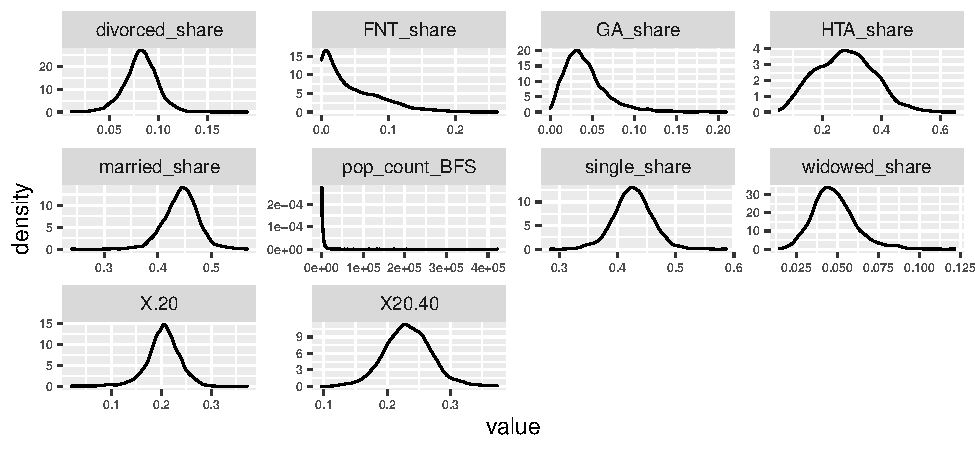
\includegraphics{Lin_Mod_Clus_Analysis_files/figure-latex/unnamed-chunk-4-1.pdf}

\begin{Shaded}
\begin{Highlighting}[]
\NormalTok{d.inf\_fac[,}\DecValTok{15}\SpecialCharTok{:}\DecValTok{26}\NormalTok{] }\SpecialCharTok{\%\textgreater{}\%}
  \FunctionTok{keep}\NormalTok{(is.numeric) }\SpecialCharTok{\%\textgreater{}\%}
  \FunctionTok{gather}\NormalTok{() }\SpecialCharTok{\%\textgreater{}\%}
  \FunctionTok{ggplot}\NormalTok{(}\FunctionTok{aes}\NormalTok{(value))  }\SpecialCharTok{+}                   \CommentTok{\# Plot the values}
    \FunctionTok{facet\_wrap}\NormalTok{(}\SpecialCharTok{\textasciitilde{}}\NormalTok{ key, }\AttributeTok{scales =} \StringTok{"free"}\NormalTok{) }\SpecialCharTok{+}  \CommentTok{\# In separate panels}
    \FunctionTok{geom\_density}\NormalTok{() }\SpecialCharTok{+}                      \CommentTok{\# show density lines}
    \FunctionTok{theme}\NormalTok{(}\AttributeTok{axis.text=}\FunctionTok{element\_text}\NormalTok{(}\AttributeTok{size=}\DecValTok{6}\NormalTok{, }\AttributeTok{face=}\StringTok{"bold"}\NormalTok{)) }\CommentTok{\# change axis size}
\end{Highlighting}
\end{Shaded}

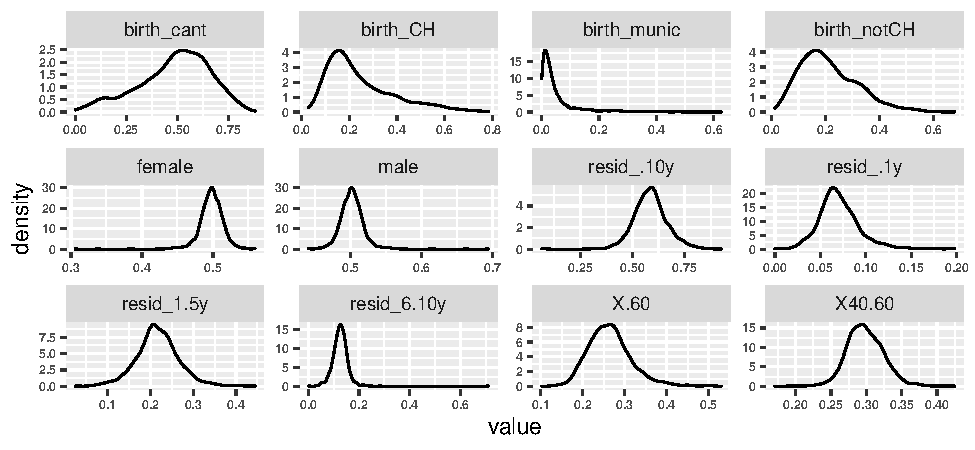
\includegraphics{Lin_Mod_Clus_Analysis_files/figure-latex/unnamed-chunk-4-2.pdf}

\begin{Shaded}
\begin{Highlighting}[]
\NormalTok{d.inf\_fac[,}\DecValTok{27}\SpecialCharTok{:}\DecValTok{38}\NormalTok{] }\SpecialCharTok{\%\textgreater{}\%}
  \FunctionTok{keep}\NormalTok{(is.numeric) }\SpecialCharTok{\%\textgreater{}\%}
  \FunctionTok{gather}\NormalTok{() }\SpecialCharTok{\%\textgreater{}\%}
  \FunctionTok{ggplot}\NormalTok{(}\FunctionTok{aes}\NormalTok{(value))  }\SpecialCharTok{+}                   \CommentTok{\# Plot the values}
    \FunctionTok{facet\_wrap}\NormalTok{(}\SpecialCharTok{\textasciitilde{}}\NormalTok{ key, }\AttributeTok{scales =} \StringTok{"free"}\NormalTok{) }\SpecialCharTok{+}  \CommentTok{\# In separate panels}
    \FunctionTok{geom\_density}\NormalTok{() }\SpecialCharTok{+}                      \CommentTok{\# show density lines}
    \FunctionTok{theme}\NormalTok{(}\AttributeTok{axis.text=}\FunctionTok{element\_text}\NormalTok{(}\AttributeTok{size=}\DecValTok{6}\NormalTok{, }\AttributeTok{face=}\StringTok{"bold"}\NormalTok{)) }\CommentTok{\# change axis size}
\end{Highlighting}
\end{Shaded}

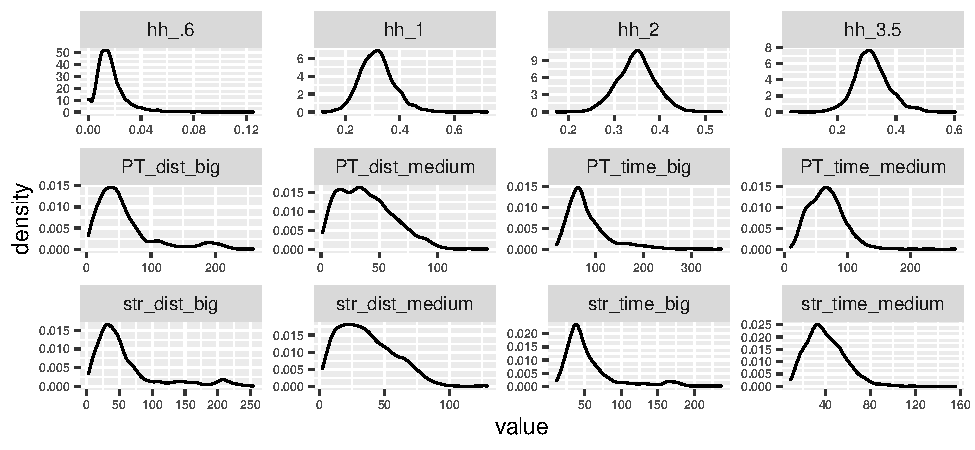
\includegraphics{Lin_Mod_Clus_Analysis_files/figure-latex/unnamed-chunk-4-3.pdf}

\begin{Shaded}
\begin{Highlighting}[]
\NormalTok{d.inf\_fac[,}\DecValTok{39}\SpecialCharTok{:}\DecValTok{50}\NormalTok{] }\SpecialCharTok{\%\textgreater{}\%}
  \FunctionTok{keep}\NormalTok{(is.numeric) }\SpecialCharTok{\%\textgreater{}\%}
  \FunctionTok{gather}\NormalTok{() }\SpecialCharTok{\%\textgreater{}\%}
  \FunctionTok{ggplot}\NormalTok{(}\FunctionTok{aes}\NormalTok{(value))  }\SpecialCharTok{+}                   \CommentTok{\# Plot the values}
    \FunctionTok{facet\_wrap}\NormalTok{(}\SpecialCharTok{\textasciitilde{}}\NormalTok{ key, }\AttributeTok{scales =} \StringTok{"free"}\NormalTok{) }\SpecialCharTok{+}  \CommentTok{\# In separate panels}
    \FunctionTok{geom\_density}\NormalTok{() }\SpecialCharTok{+}                      \CommentTok{\# show density lines}
    \FunctionTok{theme}\NormalTok{(}\AttributeTok{axis.text=}\FunctionTok{element\_text}\NormalTok{(}\AttributeTok{size=}\DecValTok{6}\NormalTok{, }\AttributeTok{face=}\StringTok{"bold"}\NormalTok{)) }\CommentTok{\# change axis size}
\end{Highlighting}
\end{Shaded}

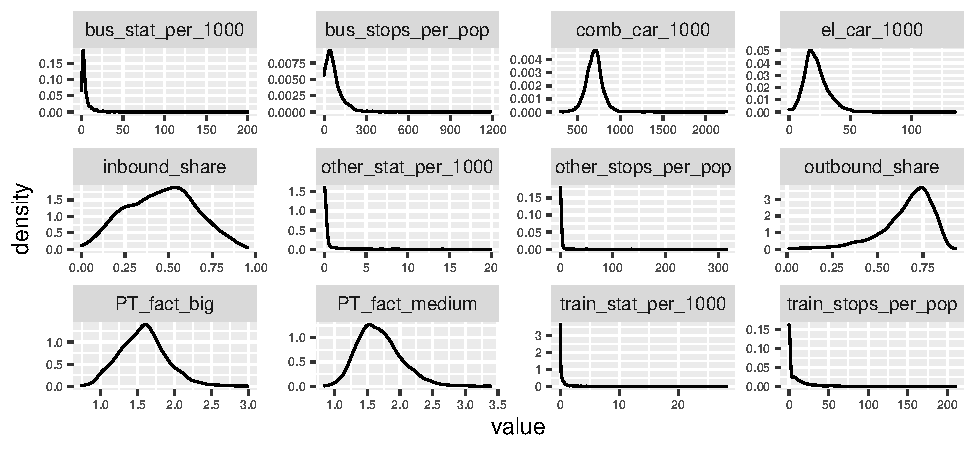
\includegraphics{Lin_Mod_Clus_Analysis_files/figure-latex/unnamed-chunk-4-4.pdf}

When looking at the graphs, it quickly becomes apparent that some
variables should be normalised so that they do not have too much weight.
Thus, the data set is created as a normalized copy afterwards:

\hypertarget{normalizing-variables}{%
\subsection{Normalizing variables}\label{normalizing-variables}}

The normalization is important due to some outstanding variables.
However, this mainly affects those variables that have no shares, as
these already lie between 0 and 1 anyway. But to standardize all
continuous variables at the same scale, I will include all parameters
except the target variable into the normalization:. A normal scale
function should do the necessary normalization in these cases.

\begin{Shaded}
\begin{Highlighting}[]
\NormalTok{d.norm }\OtherTok{\textless{}{-}}\NormalTok{ d.inf\_fac[,}\DecValTok{4}\SpecialCharTok{:}\DecValTok{50}\NormalTok{]}
\FunctionTok{print}\NormalTok{(}\FunctionTok{colnames}\NormalTok{(d.norm))}
\end{Highlighting}
\end{Shaded}

\begin{verbatim}
##  [1] "language"            "pop_count_BFS"       "single_share"       
##  [4] "married_share"       "widowed_share"       "divorced_share"     
##  [7] "GA_share"            "HTA_share"           "FNT_share"          
## [10] "X.20"                "X20.40"              "X40.60"             
## [13] "X.60"                "birth_munic"         "birth_cant"         
## [16] "birth_CH"            "birth_notCH"         "male"               
## [19] "female"              "resid_.1y"           "resid_1.5y"         
## [22] "resid_6.10y"         "resid_.10y"          "hh_1"               
## [25] "hh_2"                "hh_3.5"              "hh_.6"              
## [28] "PT_dist_medium"      "PT_time_medium"      "PT_dist_big"        
## [31] "PT_time_big"         "str_dist_medium"     "str_time_medium"    
## [34] "str_dist_big"        "str_time_big"        "PT_fact_big"        
## [37] "PT_fact_medium"      "bus_stops_per_pop"   "train_stops_per_pop"
## [40] "other_stops_per_pop" "bus_stat_per_1000"   "train_stat_per_1000"
## [43] "other_stat_per_1000" "comb_car_1000"       "el_car_1000"        
## [46] "inbound_share"       "outbound_share"
\end{verbatim}

\begin{Shaded}
\begin{Highlighting}[]
\CommentTok{\# define columns to log{-}transform:}
\NormalTok{columns }\OtherTok{\textless{}{-}} \FunctionTok{c}\NormalTok{(}\StringTok{"pop\_count\_BFS"}\NormalTok{, }\StringTok{"single\_share"}\NormalTok{, }\StringTok{"married\_share"}\NormalTok{,}
             \StringTok{"widowed\_share"}\NormalTok{, }\StringTok{"divorced\_share"}\NormalTok{, }\StringTok{"HTA\_share"}\NormalTok{,}
             \StringTok{"FNT\_share"}\NormalTok{, }\StringTok{"X.20"}\NormalTok{, }\StringTok{"X20.40"}\NormalTok{, }\StringTok{"X40.60"}\NormalTok{, }\StringTok{"X.60"}\NormalTok{, }\StringTok{"birth\_munic"}\NormalTok{,}
             \StringTok{"birth\_cant"}\NormalTok{, }\StringTok{"birth\_CH"}\NormalTok{, }\StringTok{"birth\_notCH"}\NormalTok{, }\StringTok{"male"}\NormalTok{, }\StringTok{"female"}\NormalTok{, }
             \StringTok{"resid\_.1y"}\NormalTok{, }\StringTok{"resid\_1.5y"}\NormalTok{, }\StringTok{"resid\_6.10y"}\NormalTok{, }\StringTok{"resid\_.10y"}\NormalTok{,}
             \StringTok{"hh\_1"}\NormalTok{, }\StringTok{"hh\_2"}\NormalTok{, }\StringTok{"hh\_3.5"}\NormalTok{, }\StringTok{"hh\_.6"}\NormalTok{,}
             \StringTok{"PT\_dist\_medium"}\NormalTok{, }\StringTok{"PT\_time\_medium"}\NormalTok{, }\StringTok{"PT\_dist\_big"}\NormalTok{,}
             \StringTok{"PT\_time\_big"}\NormalTok{, }\StringTok{"str\_dist\_medium"}\NormalTok{, }\StringTok{"str\_time\_medium"}\NormalTok{, }
             \StringTok{"str\_dist\_big"}\NormalTok{, }\StringTok{"str\_time\_big"}\NormalTok{, }\StringTok{"PT\_fact\_big"}\NormalTok{, }\StringTok{"PT\_fact\_medium"}\NormalTok{,}
             \StringTok{"bus\_stops\_per\_pop"}\NormalTok{, }\StringTok{"train\_stops\_per\_pop"}\NormalTok{, }\StringTok{"other\_stops\_per\_pop"}\NormalTok{,}
             \StringTok{"bus\_stat\_per\_1000"}\NormalTok{, }\StringTok{"train\_stat\_per\_1000"}\NormalTok{, }\StringTok{"other\_stat\_per\_1000"}\NormalTok{,}
             \StringTok{"comb\_car\_1000"}\NormalTok{, }\StringTok{"el\_car\_1000"}\NormalTok{, }\StringTok{"inbound\_share"}\NormalTok{, }\StringTok{"outbound\_share"}\NormalTok{)}
\FunctionTok{length}\NormalTok{(columns)}
\end{Highlighting}
\end{Shaded}

\begin{verbatim}
## [1] 45
\end{verbatim}

\begin{Shaded}
\begin{Highlighting}[]
\NormalTok{d.norm[columns] }\OtherTok{\textless{}{-}} \FunctionTok{scale}\NormalTok{(d.norm[columns])}
\FunctionTok{summary}\NormalTok{(d.norm)}
\end{Highlighting}
\end{Shaded}

\begin{verbatim}
##    language         pop_count_BFS       single_share       married_share     
##  Length:2148        Min.   :-0.31088   Min.   :-4.376545   Min.   :-6.44424  
##  Class :character   1st Qu.:-0.25372   1st Qu.:-0.618384   1st Qu.:-0.60279  
##  Mode  :character   Median :-0.18712   Median : 0.003384   Median : 0.04143  
##                     Mean   : 0.00000   Mean   : 0.000000   Mean   : 0.00000  
##                     3rd Qu.:-0.00808   3rd Qu.: 0.629999   3rd Qu.: 0.63013  
##                     Max.   :32.18958   Max.   : 4.950234   Max.   : 3.88560  
##                                        NA's   :1           NA's   :1         
##  widowed_share     divorced_share        GA_share         HTA_share       
##  Min.   :-2.5686   Min.   :-4.11901   Min.   :0.00000   Min.   :-2.32960  
##  1st Qu.:-0.6692   1st Qu.:-0.57369   1st Qu.:0.02416   1st Qu.:-0.75725  
##  Median :-0.1062   Median : 0.01449   Median :0.03647   Median : 0.00544  
##  Mean   : 0.0000   Mean   : 0.00000   Mean   :0.04171   Mean   : 0.00000  
##  3rd Qu.: 0.5382   3rd Qu.: 0.60733   3rd Qu.:0.05243   3rd Qu.: 0.68823  
##  Max.   : 5.6364   Max.   : 6.29086   Max.   :0.20916   Max.   : 3.88430  
##  NA's   :1         NA's   :1          NA's   :1         NA's   :1         
##    FNT_share            X.20              X20.40             X40.60        
##  Min.   :-0.9836   Min.   :-5.47538   Min.   :-3.70295   Min.   :-4.88516  
##  1st Qu.:-0.8205   1st Qu.:-0.51941   1st Qu.:-0.65825   1st Qu.:-0.66324  
##  Median :-0.3485   Median : 0.04636   Median :-0.02065   Median :-0.06739  
##  Mean   : 0.0000   Mean   : 0.00000   Mean   : 0.00000   Mean   : 0.00000  
##  3rd Qu.: 0.5970   3rd Qu.: 0.59245   3rd Qu.: 0.62955   3rd Qu.: 0.64575  
##  Max.   : 5.1117   Max.   : 5.01639   Max.   : 3.82754   Max.   : 4.82421  
##  NA's   :1         NA's   :11         NA's   :11         NA's   :11        
##       X.60           birth_munic         birth_cant         birth_CH      
##  Min.   :-3.11518   Min.   :-0.70050   Min.   :-2.8192   Min.   :-1.5231  
##  1st Qu.:-0.67303   1st Qu.:-0.53510   1st Qu.:-0.6196   1st Qu.:-0.7350  
##  Median :-0.07741   Median :-0.35167   Median : 0.1365   Median :-0.3111  
##  Mean   : 0.00000   Mean   : 0.00000   Mean   : 0.0000   Mean   : 0.0000  
##  3rd Qu.: 0.53002   3rd Qu.: 0.02665   3rd Qu.: 0.7240   3rd Qu.: 0.5112  
##  Max.   : 5.09044   Max.   : 7.36914   Max.   : 2.2772   Max.   : 3.7513  
##  NA's   :11         NA's   :11         NA's   :11        NA's   :11       
##   birth_notCH           male              female            resid_.1y      
##  Min.   :-1.8829   Min.   :-3.63319   Min.   :-11.35691   Min.   :-3.0788  
##  1st Qu.:-0.7461   1st Qu.:-0.58628   1st Qu.: -0.51165   1st Qu.:-0.6111  
##  Median :-0.1741   Median :-0.03668   Median :  0.03668   Median :-0.1141  
##  Mean   : 0.0000   Mean   : 0.00000   Mean   :  0.00000   Mean   : 0.0000  
##  3rd Qu.: 0.6378   3rd Qu.: 0.51165   3rd Qu.:  0.58628   3rd Qu.: 0.5068  
##  Max.   : 4.3941   Max.   :11.35691   Max.   :  3.63319   Max.   : 5.5222  
##  NA's   :11        NA's   :11         NA's   :11          NA's   :11       
##    resid_1.5y        resid_6.10y         resid_.10y           hh_1         
##  Min.   :-3.84468   Min.   :-3.45583   Min.   :-6.4191   Min.   :-3.19201  
##  1st Qu.:-0.58995   1st Qu.:-0.47400   1st Qu.:-0.6097   1st Qu.:-0.67078  
##  Median :-0.03538   Median :-0.01947   Median :-0.0214   Median :-0.05555  
##  Mean   : 0.00000   Mean   : 0.00000   Mean   : 0.0000   Mean   : 0.00000  
##  3rd Qu.: 0.58038   3rd Qu.: 0.42418   3rd Qu.: 0.5663   3rd Qu.: 0.56745  
##  Max.   : 4.54704   Max.   :16.01102   Max.   : 4.1911   Max.   : 6.41521  
##  NA's   :11         NA's   :11         NA's   :11        NA's   :11        
##       hh_2               hh_3.5             hh_.6         PT_dist_medium   
##  Min.   :-4.139633   Min.   :-4.69615   Min.   :-1.4949   Min.   :-1.6311  
##  1st Qu.:-0.619733   1st Qu.:-0.61957   1st Qu.:-0.6072   1st Qu.:-0.8161  
##  Median : 0.002849   Median :-0.07343   Median :-0.1819   Median :-0.1295  
##  Mean   : 0.000000   Mean   : 0.00000   Mean   : 0.0000   Mean   : 0.0000  
##  3rd Qu.: 0.613243   3rd Qu.: 0.57888   3rd Qu.: 0.3385   3rd Qu.: 0.6550  
##  Max.   : 4.382765   Max.   : 4.84774   Max.   : 9.6584   Max.   : 4.5213  
##  NA's   :11          NA's   :11         NA's   :11        NA's   :34       
##  PT_time_medium      PT_dist_big       PT_time_big      str_dist_medium  
##  Min.   :-2.06968   Min.   :-1.1777   Min.   :-1.4436   Min.   :-1.6020  
##  1st Qu.:-0.73858   1st Qu.:-0.6350   1st Qu.:-0.6371   1st Qu.:-0.8075  
##  Median :-0.05916   Median :-0.2814   Median :-0.2682   Median :-0.1444  
##  Mean   : 0.00000   Mean   : 0.0000   Mean   : 0.0000   Mean   : 0.0000  
##  3rd Qu.: 0.59984   3rd Qu.: 0.2247   3rd Qu.: 0.3482   3rd Qu.: 0.6780  
##  Max.   : 7.41852   Max.   : 4.2470   Max.   : 6.2701   Max.   : 4.4209  
##  NA's   :34         NA's   :34        NA's   :34        NA's   :34       
##  str_time_medium    str_dist_big      str_time_big      PT_fact_big     
##  Min.   :-1.8049   Min.   :-1.0813   Min.   :-1.1851   Min.   :-2.6218  
##  1st Qu.:-0.7050   1st Qu.:-0.6043   1st Qu.:-0.5920   1st Qu.:-0.6767  
##  Median :-0.1334   Median :-0.3082   Median :-0.3194   Median :-0.0131  
##  Mean   : 0.0000   Mean   : 0.0000   Mean   : 0.0000   Mean   : 0.0000  
##  3rd Qu.: 0.6112   3rd Qu.: 0.1516   3rd Qu.: 0.1880   3rd Qu.: 0.5835  
##  Max.   : 6.6460   Max.   : 3.8736   Max.   : 4.8275   Max.   : 4.4256  
##  NA's   :34        NA's   :34        NA's   :34        NA's   :34       
##  PT_fact_medium    bus_stops_per_pop train_stops_per_pop other_stops_per_pop
##  Min.   :-2.5333   Min.   :-0.9932   Min.   :-0.4902     Min.   :-0.09163   
##  1st Qu.:-0.7100   1st Qu.:-0.6110   1st Qu.:-0.4902     1st Qu.:-0.09163   
##  Median :-0.1125   Median :-0.2303   Median :-0.4902     Median :-0.09163   
##  Mean   : 0.0000   Mean   : 0.0000   Mean   : 0.0000     Mean   : 0.00000   
##  3rd Qu.: 0.5730   3rd Qu.: 0.3118   3rd Qu.: 0.1319     3rd Qu.:-0.09163   
##  Max.   : 5.0946   Max.   :15.9957   Max.   :12.9081     Max.   :28.95660   
##  NA's   :34        NA's   :67        NA's   :67          NA's   :67         
##  bus_stat_per_1000 train_stat_per_1000 other_stat_per_1000 comb_car_1000     
##  Min.   :-0.5978   Min.   :-0.33025    Min.   :-0.2034     Min.   :-3.46868  
##  1st Qu.:-0.4089   1st Qu.:-0.33025    1st Qu.:-0.2034     1st Qu.:-0.54423  
##  Median :-0.2609   Median :-0.33025    Median :-0.2034     Median :-0.03329  
##  Mean   : 0.0000   Mean   : 0.00000    Mean   : 0.0000     Mean   : 0.00000  
##  3rd Qu.: 0.0449   3rd Qu.:-0.02053    3rd Qu.:-0.2034     3rd Qu.: 0.43391  
##  Max.   :22.1024   Max.   :25.17166    Max.   :17.6480     Max.   :13.27683  
##  NA's   :67        NA's   :67          NA's   :67          NA's   :11        
##   el_car_1000      inbound_share     outbound_share   
##  Min.   :-2.1878   Min.   :-2.3414   Min.   :-4.4670  
##  1st Qu.:-0.6397   1st Qu.:-0.7649   1st Qu.:-0.4416  
##  Median :-0.1364   Median : 0.0404   Median : 0.2201  
##  Mean   : 0.0000   Mean   : 0.0000   Mean   : 0.0000  
##  3rd Qu.: 0.4818   3rd Qu.: 0.7113   3rd Qu.: 0.6930  
##  Max.   :11.2338   Max.   : 2.5201   Max.   : 1.8279  
##  NA's   :11        NA's   :133       NA's   :133
\end{verbatim}

\hypertarget{correlation-charts-to-factor-groups}{%
\subsection{Correlation charts to factor
groups}\label{correlation-charts-to-factor-groups}}

\hypertarget{marital-state}{%
\subsubsection{Marital state}\label{marital-state}}

\begin{Shaded}
\begin{Highlighting}[]
\FunctionTok{chart.Correlation}\NormalTok{(d.inf\_fac[,}\FunctionTok{c}\NormalTok{(}\DecValTok{10}\SpecialCharTok{:}\DecValTok{12}\NormalTok{, }\DecValTok{6}\SpecialCharTok{:}\DecValTok{9}\NormalTok{)], }\CommentTok{\# +1 due to 0{-}values (log(0) = {-}Inf)}
                  \AttributeTok{histogram=}\ConstantTok{TRUE}\NormalTok{) }\CommentTok{\# adding histograms to the plot}
\end{Highlighting}
\end{Shaded}

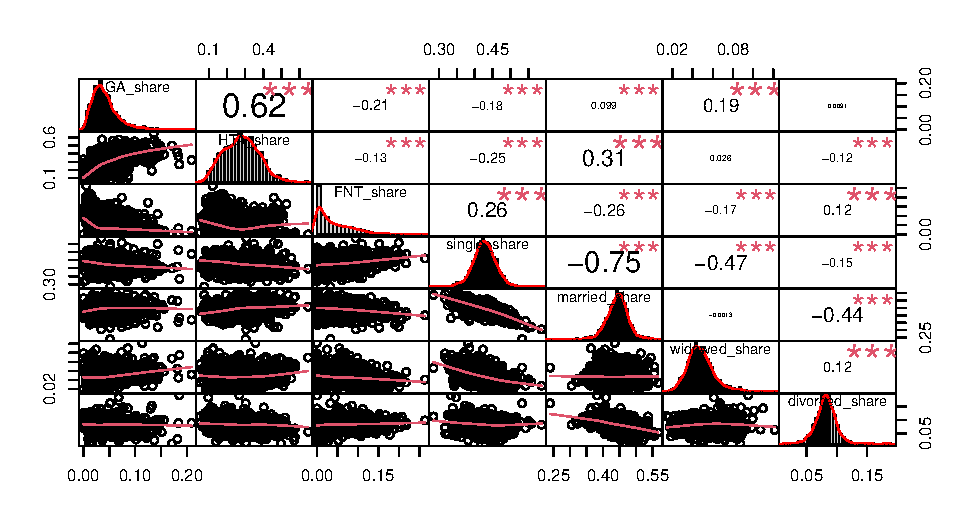
\includegraphics{Lin_Mod_Clus_Analysis_files/figure-latex/unnamed-chunk-6-1.pdf}

\hypertarget{age-segment}{%
\subsubsection{Age segment}\label{age-segment}}

\begin{Shaded}
\begin{Highlighting}[]
\FunctionTok{chart.Correlation}\NormalTok{(d.inf\_fac[,}\FunctionTok{c}\NormalTok{(}\DecValTok{10}\SpecialCharTok{:}\DecValTok{12}\NormalTok{, }\DecValTok{13}\SpecialCharTok{:}\DecValTok{16}\NormalTok{)], }\CommentTok{\# +1 due to 0{-}values (log(0) = {-}Inf)}
                  \AttributeTok{histogram=}\ConstantTok{TRUE}\NormalTok{) }\CommentTok{\# adding histograms to the plot}
\end{Highlighting}
\end{Shaded}

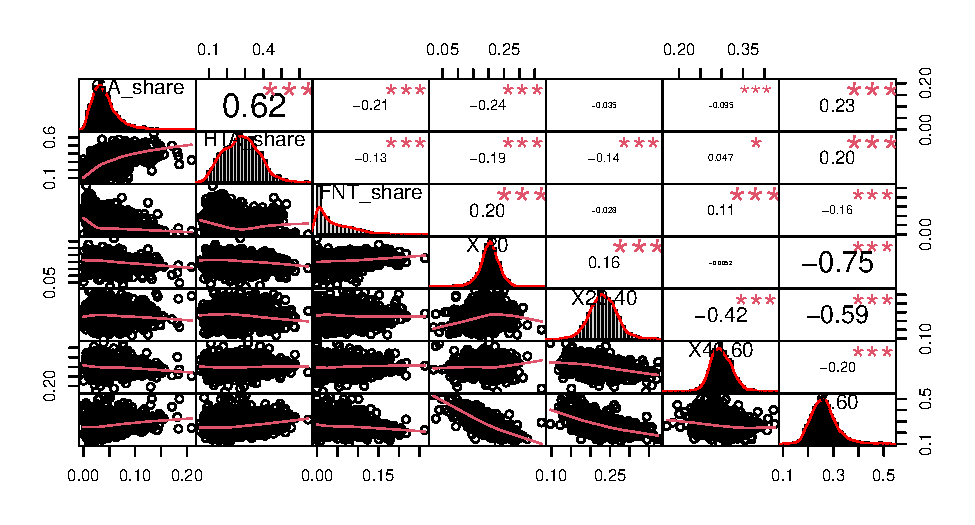
\includegraphics{Lin_Mod_Clus_Analysis_files/figure-latex/unnamed-chunk-7-1.pdf}

\hypertarget{birth-origin}{%
\subsubsection{Birth origin}\label{birth-origin}}

\begin{Shaded}
\begin{Highlighting}[]
\FunctionTok{chart.Correlation}\NormalTok{(d.inf\_fac[,}\FunctionTok{c}\NormalTok{(}\DecValTok{10}\SpecialCharTok{:}\DecValTok{12}\NormalTok{, }\DecValTok{17}\SpecialCharTok{:}\DecValTok{20}\NormalTok{)], }\CommentTok{\# +1 due to 0{-}values (log(0) = {-}Inf)}
                  \AttributeTok{histogram=}\ConstantTok{TRUE}\NormalTok{) }\CommentTok{\# adding histograms to the plot}
\end{Highlighting}
\end{Shaded}

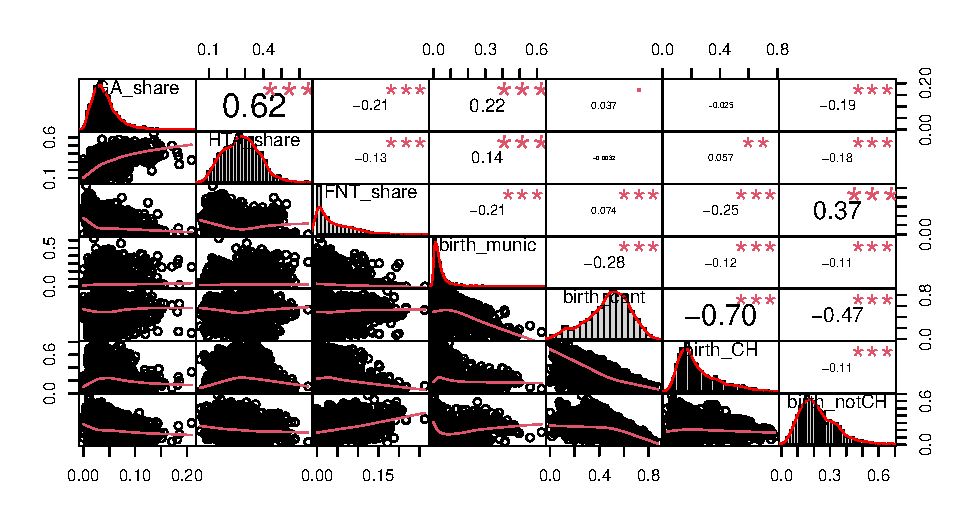
\includegraphics{Lin_Mod_Clus_Analysis_files/figure-latex/unnamed-chunk-8-1.pdf}

\hypertarget{gender}{%
\subsubsection{Gender}\label{gender}}

\begin{Shaded}
\begin{Highlighting}[]
\FunctionTok{chart.Correlation}\NormalTok{(d.inf\_fac[,}\FunctionTok{c}\NormalTok{(}\DecValTok{10}\SpecialCharTok{:}\DecValTok{12}\NormalTok{, }\DecValTok{21}\SpecialCharTok{:}\DecValTok{22}\NormalTok{)], }\CommentTok{\# +1 due to 0{-}values (log(0) = {-}Inf)}
                  \AttributeTok{histogram=}\ConstantTok{TRUE}\NormalTok{) }\CommentTok{\# adding histograms to the plot}
\end{Highlighting}
\end{Shaded}

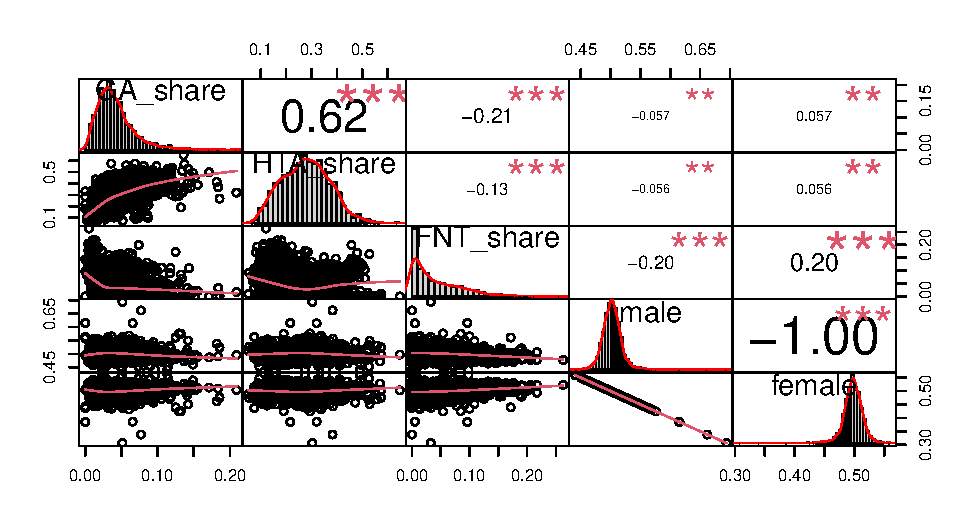
\includegraphics{Lin_Mod_Clus_Analysis_files/figure-latex/unnamed-chunk-9-1.pdf}

\hypertarget{residence-time}{%
\subsubsection{Residence time}\label{residence-time}}

\begin{Shaded}
\begin{Highlighting}[]
\FunctionTok{chart.Correlation}\NormalTok{(d.inf\_fac[,}\FunctionTok{c}\NormalTok{(}\DecValTok{10}\SpecialCharTok{:}\DecValTok{12}\NormalTok{, }\DecValTok{23}\SpecialCharTok{:}\DecValTok{26}\NormalTok{)], }\CommentTok{\# +1 due to 0{-}values (log(0) = {-}Inf)}
                  \AttributeTok{histogram=}\ConstantTok{TRUE}\NormalTok{) }\CommentTok{\# adding histograms to the plot}
\end{Highlighting}
\end{Shaded}

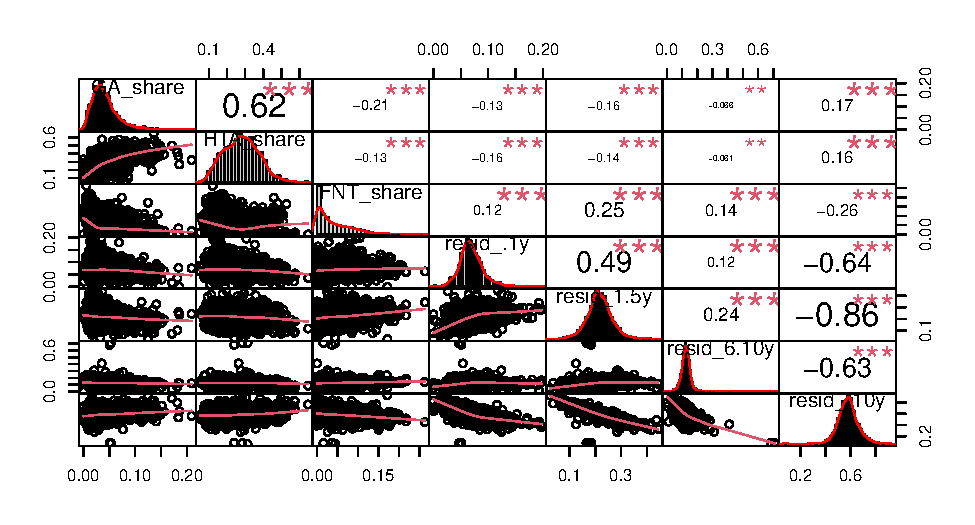
\includegraphics{Lin_Mod_Clus_Analysis_files/figure-latex/unnamed-chunk-10-1.pdf}

\hypertarget{household-size}{%
\subsubsection{Household size}\label{household-size}}

\begin{Shaded}
\begin{Highlighting}[]
\FunctionTok{chart.Correlation}\NormalTok{(d.inf\_fac[,}\FunctionTok{c}\NormalTok{(}\DecValTok{10}\SpecialCharTok{:}\DecValTok{12}\NormalTok{, }\DecValTok{27}\SpecialCharTok{:}\DecValTok{30}\NormalTok{)], }\CommentTok{\# +1 due to 0{-}values (log(0) = {-}Inf)}
                  \AttributeTok{histogram=}\ConstantTok{TRUE}\NormalTok{) }\CommentTok{\# adding histograms to the plot}
\end{Highlighting}
\end{Shaded}

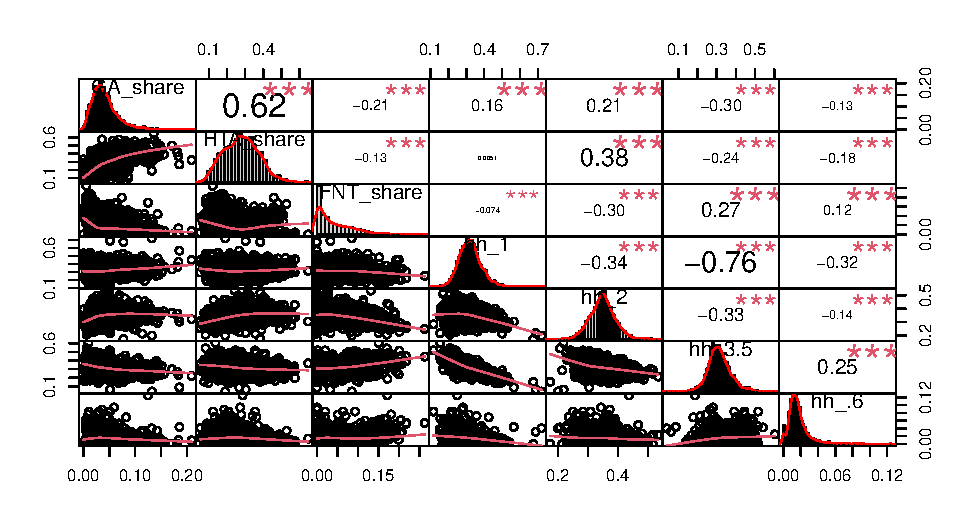
\includegraphics{Lin_Mod_Clus_Analysis_files/figure-latex/unnamed-chunk-11-1.pdf}

\hypertarget{pt-distance-and-time-to-middlebig-cities}{%
\subsubsection{PT Distance and time to middle/big
cities}\label{pt-distance-and-time-to-middlebig-cities}}

\begin{Shaded}
\begin{Highlighting}[]
\FunctionTok{chart.Correlation}\NormalTok{(d.inf\_fac[,}\FunctionTok{c}\NormalTok{(}\DecValTok{10}\SpecialCharTok{:}\DecValTok{12}\NormalTok{, }\DecValTok{31}\SpecialCharTok{:}\DecValTok{34}\NormalTok{)], }\CommentTok{\# +1 due to 0{-}values (log(0) = {-}Inf)}
                  \AttributeTok{histogram=}\ConstantTok{TRUE}\NormalTok{) }\CommentTok{\# adding histograms to the plot}
\end{Highlighting}
\end{Shaded}

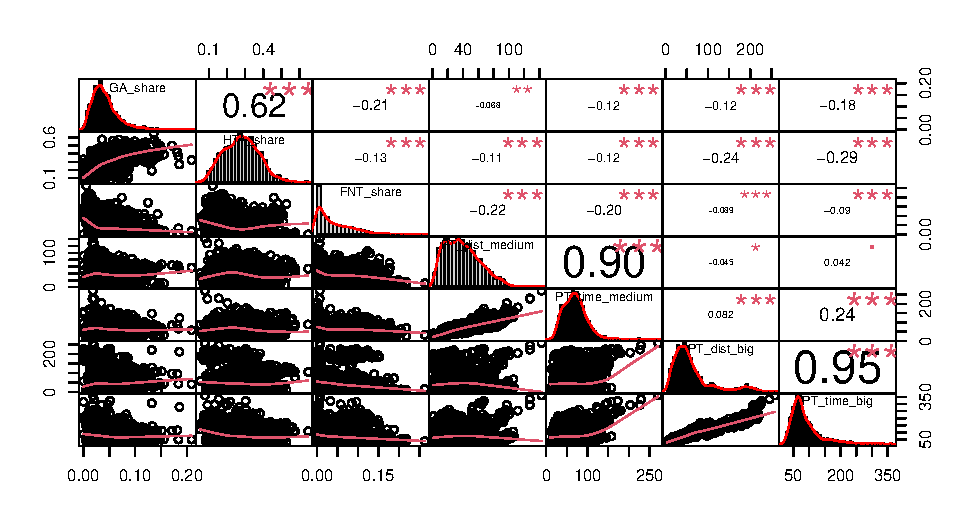
\includegraphics{Lin_Mod_Clus_Analysis_files/figure-latex/unnamed-chunk-12-1.pdf}
\#\#\# PT Factor compared to Street (Time consumption)

\begin{Shaded}
\begin{Highlighting}[]
\FunctionTok{chart.Correlation}\NormalTok{(d.inf\_fac[,}\FunctionTok{c}\NormalTok{(}\DecValTok{10}\SpecialCharTok{:}\DecValTok{12}\NormalTok{, }\DecValTok{39}\SpecialCharTok{:}\DecValTok{40}\NormalTok{)], }\CommentTok{\# +1 due to 0{-}values (log(0) = {-}Inf)}
                  \AttributeTok{histogram=}\ConstantTok{TRUE}\NormalTok{) }\CommentTok{\# adding histograms to the plot}
\end{Highlighting}
\end{Shaded}

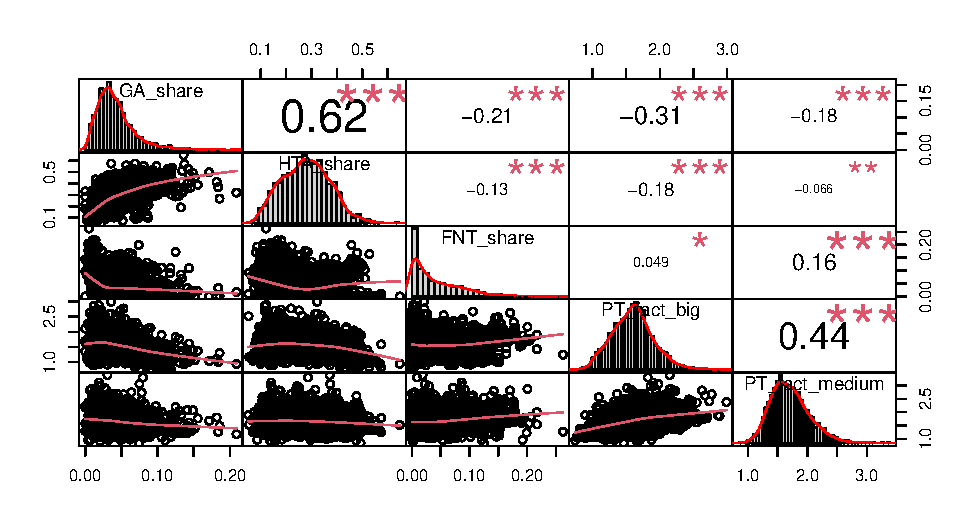
\includegraphics{Lin_Mod_Clus_Analysis_files/figure-latex/unnamed-chunk-13-1.pdf}

\hypertarget{bus-train-other-stops-per-population}{%
\subsubsection{Bus / train / other stops per
population}\label{bus-train-other-stops-per-population}}

\begin{Shaded}
\begin{Highlighting}[]
\FunctionTok{chart.Correlation}\NormalTok{(}\FunctionTok{log}\NormalTok{(d.inf\_fac[,}\FunctionTok{c}\NormalTok{(}\DecValTok{10}\SpecialCharTok{:}\DecValTok{12}\NormalTok{, }\DecValTok{5}\NormalTok{, }\DecValTok{41}\SpecialCharTok{:}\DecValTok{45}\NormalTok{)]}\SpecialCharTok{+}\DecValTok{1}\NormalTok{), }\CommentTok{\# +1 due to 0{-}values (log(0) = {-}Inf)}
                  \AttributeTok{histogram=}\ConstantTok{TRUE}\NormalTok{) }\CommentTok{\# adding histograms to the plot}
\end{Highlighting}
\end{Shaded}

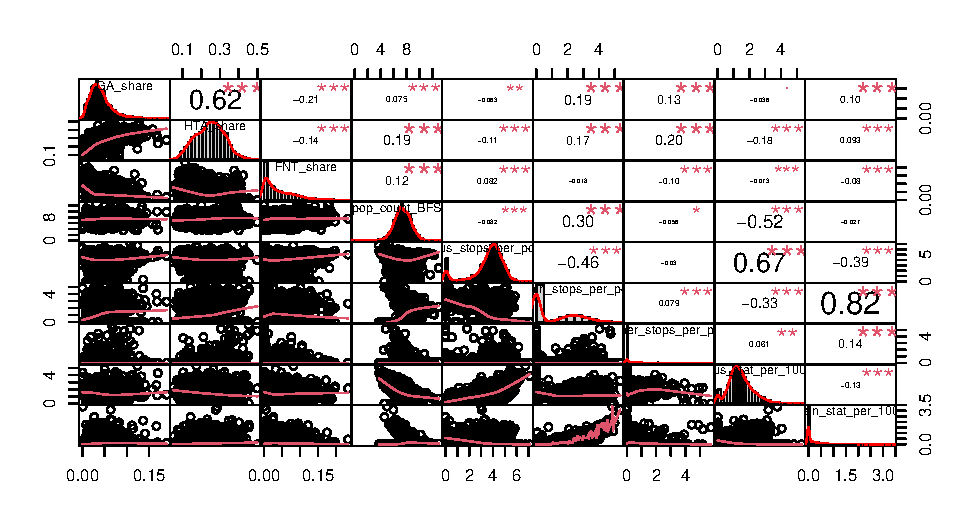
\includegraphics{Lin_Mod_Clus_Analysis_files/figure-latex/unnamed-chunk-14-1.pdf}

\hypertarget{car-distribution}{%
\subsubsection{Car distribution}\label{car-distribution}}

\begin{Shaded}
\begin{Highlighting}[]
\FunctionTok{chart.Correlation}\NormalTok{(d.inf\_fac[,}\FunctionTok{c}\NormalTok{(}\DecValTok{10}\SpecialCharTok{:}\DecValTok{12}\NormalTok{, }\DecValTok{47}\SpecialCharTok{:}\DecValTok{48}\NormalTok{)], }\CommentTok{\# +1 due to 0{-}values (log(0) = {-}Inf)}
                  \AttributeTok{histogram=}\ConstantTok{TRUE}\NormalTok{) }\CommentTok{\# adding histograms to the plot}
\end{Highlighting}
\end{Shaded}

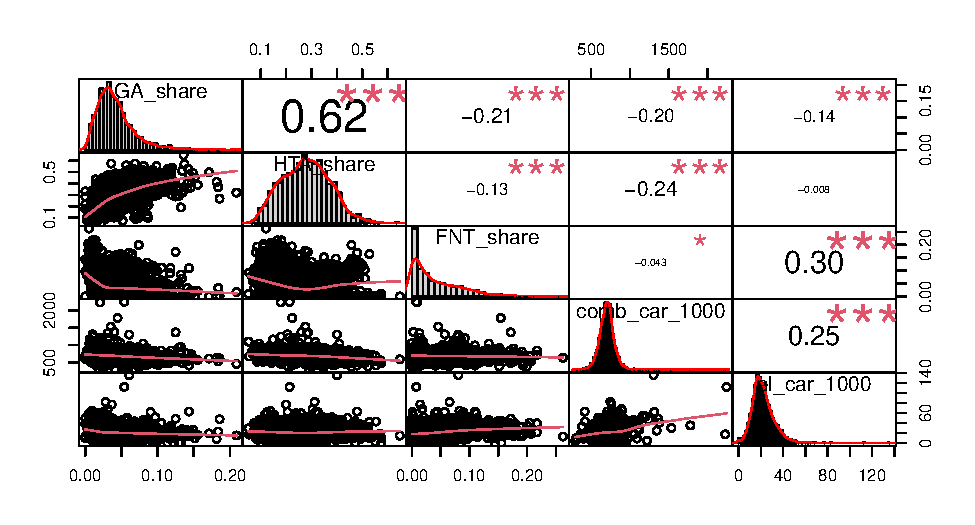
\includegraphics{Lin_Mod_Clus_Analysis_files/figure-latex/unnamed-chunk-15-1.pdf}

\hypertarget{commuter-statistics}{%
\subsubsection{Commuter statistics}\label{commuter-statistics}}

\begin{Shaded}
\begin{Highlighting}[]
\FunctionTok{chart.Correlation}\NormalTok{(d.inf\_fac[,}\FunctionTok{c}\NormalTok{(}\DecValTok{10}\SpecialCharTok{:}\DecValTok{12}\NormalTok{, }\DecValTok{49}\SpecialCharTok{:}\DecValTok{50}\NormalTok{)], }\CommentTok{\# +1 due to 0{-}values (log(0) = {-}Inf)}
                  \AttributeTok{histogram=}\ConstantTok{TRUE}\NormalTok{) }\CommentTok{\# adding histograms to the plot}
\end{Highlighting}
\end{Shaded}

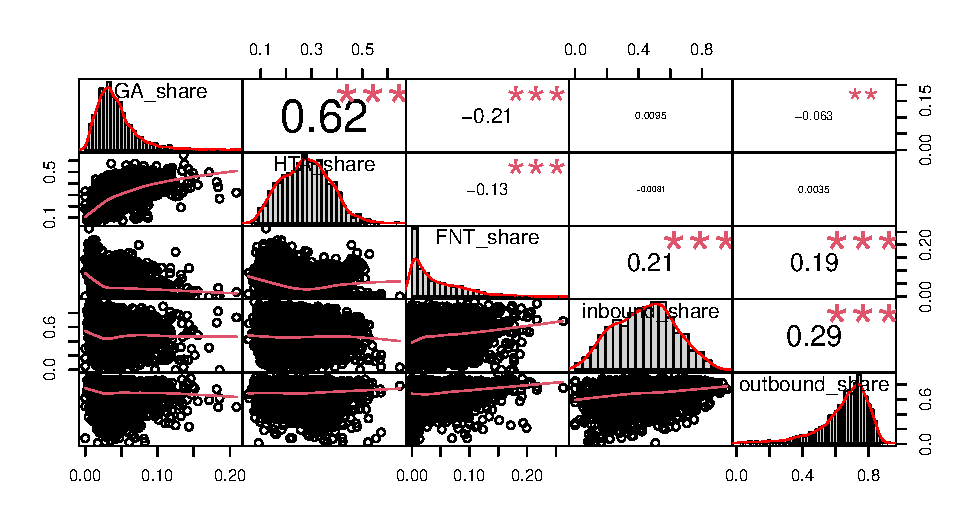
\includegraphics{Lin_Mod_Clus_Analysis_files/figure-latex/unnamed-chunk-16-1.pdf}

\hypertarget{ga-hta-fnt-shares-compared-to-languages}{%
\subsection{GA, HTA \& FNT shares compared to
languages:}\label{ga-hta-fnt-shares-compared-to-languages}}

\begin{Shaded}
\begin{Highlighting}[]
\NormalTok{plot\_HTA }\OtherTok{\textless{}{-}} \FunctionTok{ggbarplot}\NormalTok{(d.inf\_fac, }\AttributeTok{x=}\StringTok{"language"}\NormalTok{, }\AttributeTok{y=}\StringTok{"HTA\_share"}\NormalTok{, }
                      \AttributeTok{fill=}\StringTok{"language"}\NormalTok{, }
              \CommentTok{\#        facet.by="language", }
                      \AttributeTok{add =} \StringTok{"mean\_se"}\NormalTok{,}
                      \AttributeTok{xlab =} \StringTok{"language"}\NormalTok{,}
                      \AttributeTok{legend =} \StringTok{"right"}\NormalTok{,}
                      \AttributeTok{title =} \StringTok{"HTA"}\NormalTok{,}
                      \AttributeTok{ggtheme =} \FunctionTok{theme\_cleveland}\NormalTok{()) }\SpecialCharTok{+} \CommentTok{\# better looking theme}
  \FunctionTok{theme}\NormalTok{(}\AttributeTok{axis.text=}\FunctionTok{element\_text}\NormalTok{(}\AttributeTok{size=}\FloatTok{6.5}\NormalTok{, }\AttributeTok{face=}\StringTok{"bold"}\NormalTok{))}

\NormalTok{plot\_GA }\OtherTok{\textless{}{-}} \FunctionTok{ggbarplot}\NormalTok{(d.inf\_fac, }\AttributeTok{x=}\StringTok{"language"}\NormalTok{, }\AttributeTok{y=}\StringTok{"GA\_share"}\NormalTok{, }
                      \AttributeTok{fill=}\StringTok{"language"}\NormalTok{, }
                \CommentTok{\#       facet.by="language", }
                      \AttributeTok{add =} \StringTok{"mean\_se"}\NormalTok{,}
                      \AttributeTok{xlab =} \StringTok{"language"}\NormalTok{,}
                      \AttributeTok{legend =} \StringTok{"right"}\NormalTok{,}
                      \AttributeTok{title =} \StringTok{"GA"}\NormalTok{,}
                      \AttributeTok{ggtheme =} \FunctionTok{theme\_cleveland}\NormalTok{()) }\SpecialCharTok{+}
  \FunctionTok{theme}\NormalTok{(}\AttributeTok{axis.text=}\FunctionTok{element\_text}\NormalTok{(}\AttributeTok{size=}\FloatTok{6.5}\NormalTok{, }\AttributeTok{face=}\StringTok{"bold"}\NormalTok{))}

\NormalTok{plot\_FNT }\OtherTok{\textless{}{-}} \FunctionTok{ggbarplot}\NormalTok{(d.inf\_fac, }\AttributeTok{x=}\StringTok{"language"}\NormalTok{, }\AttributeTok{y=}\StringTok{"FNT\_share"}\NormalTok{, }
                      \AttributeTok{fill=}\StringTok{"language"}\NormalTok{, }
                    \CommentTok{\#  facet.by="language", }
                      \AttributeTok{add =} \StringTok{"mean\_se"}\NormalTok{,}
                      \AttributeTok{xlab =} \StringTok{"language"}\NormalTok{,}
                      \AttributeTok{legend =} \StringTok{"right"}\NormalTok{,}
                      \AttributeTok{title =} \StringTok{"FNT"}\NormalTok{,}
                      \AttributeTok{ggtheme =} \FunctionTok{theme\_cleveland}\NormalTok{()) }\SpecialCharTok{+}
  \FunctionTok{theme}\NormalTok{(}\AttributeTok{axis.text=}\FunctionTok{element\_text}\NormalTok{(}\AttributeTok{size=}\FloatTok{6.5}\NormalTok{, }\AttributeTok{face=}\StringTok{"bold"}\NormalTok{))}


\NormalTok{share.comparison }\OtherTok{\textless{}{-}} \FunctionTok{ggarrange}\NormalTok{(plot\_GA, plot\_HTA, plot\_FNT, }\AttributeTok{ncol=}\DecValTok{3}\NormalTok{) }\CommentTok{\# two plots beside each other}

\FunctionTok{annotate\_figure}\NormalTok{(share.comparison, }
                \AttributeTok{top =} \FunctionTok{text\_grob}\NormalTok{(}\StringTok{"Comparison of mean share of GA \& }
\StringTok{                                HTA sold in \% of population"}\NormalTok{, }
                                \AttributeTok{face =} \StringTok{"bold"}\NormalTok{)) }\CommentTok{\# set over{-}all title ("top")}
\end{Highlighting}
\end{Shaded}

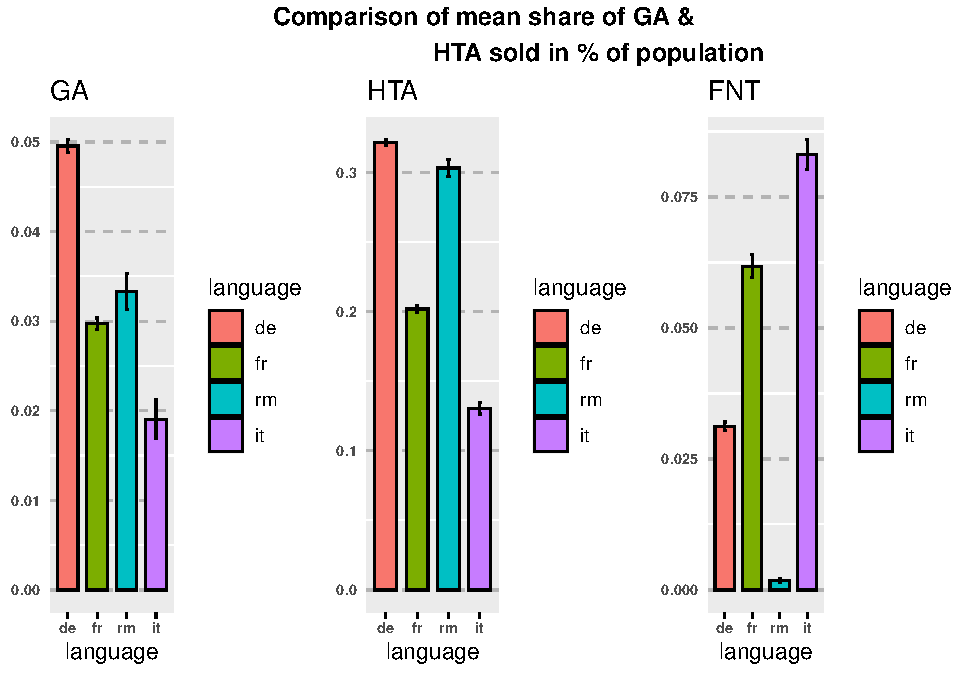
\includegraphics{Lin_Mod_Clus_Analysis_files/figure-latex/unnamed-chunk-17-1.pdf}

\newpage

\hypertarget{modelling-shares}{%
\section{MODELLING SHARES}\label{modelling-shares}}

I will achieve the first objective of modelling the share of season
tickets through two different approaches:

\hypertarget{train-test-splitting}{%
\subsection{Train / Test splitting}\label{train-test-splitting}}

\hypertarget{original-dataset}{%
\subsubsection{original dataset}\label{original-dataset}}

\begin{Shaded}
\begin{Highlighting}[]
\FunctionTok{set.seed}\NormalTok{(}\DecValTok{234}\NormalTok{) }\CommentTok{\# reproducible}
\NormalTok{indexes }\OtherTok{\textless{}{-}} \FunctionTok{createDataPartition}\NormalTok{(d.inf\_fac}\SpecialCharTok{$}\NormalTok{BFS\_Nr, }\AttributeTok{p =}\NormalTok{ .}\DecValTok{8}\NormalTok{, }\AttributeTok{list =} \ConstantTok{FALSE}\NormalTok{) }
\NormalTok{d.train }\OtherTok{\textless{}{-}}\NormalTok{ d.inf\_fac[indexes, ]}
\NormalTok{d.test }\OtherTok{\textless{}{-}}\NormalTok{ d.inf\_fac[}\SpecialCharTok{{-}}\NormalTok{indexes, ]}

\FunctionTok{sum}\NormalTok{(}\FunctionTok{length}\NormalTok{(d.train}\SpecialCharTok{$}\NormalTok{BFS\_Nr) }\SpecialCharTok{+} \FunctionTok{length}\NormalTok{(d.test}\SpecialCharTok{$}\NormalTok{BFS\_Nr)) }\CommentTok{\# control the split}
\end{Highlighting}
\end{Shaded}

\begin{verbatim}
## [1] 2148
\end{verbatim}

\begin{Shaded}
\begin{Highlighting}[]
\FunctionTok{length}\NormalTok{(d.inf\_fac}\SpecialCharTok{$}\NormalTok{BFS\_Nr)}
\end{Highlighting}
\end{Shaded}

\begin{verbatim}
## [1] 2148
\end{verbatim}

\begin{Shaded}
\begin{Highlighting}[]
\CommentTok{\# print(d.train[1:5,])}
\end{Highlighting}
\end{Shaded}

\hypertarget{normalized-dataset}{%
\subsubsection{Normalized dataset}\label{normalized-dataset}}

\begin{Shaded}
\begin{Highlighting}[]
\FunctionTok{set.seed}\NormalTok{(}\DecValTok{234}\NormalTok{) }\CommentTok{\# reproducible}
\NormalTok{indexes }\OtherTok{\textless{}{-}} \FunctionTok{createDataPartition}\NormalTok{(d.inf\_fac}\SpecialCharTok{$}\NormalTok{BFS\_Nr, }\AttributeTok{p =}\NormalTok{ .}\DecValTok{8}\NormalTok{, }\AttributeTok{list =} \ConstantTok{FALSE}\NormalTok{) }
\NormalTok{d.norm.train }\OtherTok{\textless{}{-}}\NormalTok{ d.norm[indexes, ]}
\NormalTok{d.norm.test }\OtherTok{\textless{}{-}}\NormalTok{ d.norm[}\SpecialCharTok{{-}}\NormalTok{indexes, ]}
\end{Highlighting}
\end{Shaded}

\hypertarget{function-for-model-evaluation}{%
\subsection{Function for Model
Evaluation}\label{function-for-model-evaluation}}

For the evaluation of our models we will use the following function,
which displays the RMSE and the R\_squared for our predicted values.

\begin{Shaded}
\begin{Highlighting}[]
\NormalTok{eval\_results }\OtherTok{\textless{}{-}} \ControlFlowTok{function}\NormalTok{(true, predicted) \{}
\NormalTok{  SSE }\OtherTok{\textless{}{-}} \FunctionTok{sum}\NormalTok{((predicted }\SpecialCharTok{{-}}\NormalTok{ true)}\SpecialCharTok{\^{}}\DecValTok{2}\NormalTok{, }\AttributeTok{na.rm =} \ConstantTok{TRUE}\NormalTok{)}
\NormalTok{  SST }\OtherTok{\textless{}{-}} \FunctionTok{sum}\NormalTok{((true }\SpecialCharTok{{-}} \FunctionTok{mean}\NormalTok{(true, }\AttributeTok{na.rm =} \ConstantTok{TRUE}\NormalTok{))}\SpecialCharTok{\^{}}\DecValTok{2}\NormalTok{, }\AttributeTok{na.rm =} \ConstantTok{TRUE}\NormalTok{)}
\NormalTok{  R\_square }\OtherTok{\textless{}{-}} \DecValTok{1} \SpecialCharTok{{-}}\NormalTok{ SSE }\SpecialCharTok{/}\NormalTok{ SST}
\NormalTok{  RMSE }\OtherTok{=} \FunctionTok{sqrt}\NormalTok{(SSE}\SpecialCharTok{/}\FunctionTok{length}\NormalTok{(true))}

\CommentTok{\# Model performance metrics}
\FunctionTok{data.frame}\NormalTok{(}\AttributeTok{RMSE =}\NormalTok{ RMSE,}
           \AttributeTok{Rsquare =}\NormalTok{ R\_square)}
\NormalTok{\}}
\end{Highlighting}
\end{Shaded}

\hypertarget{linear-model}{%
\subsection{Linear model}\label{linear-model}}

The first method is a classic linear model that models the absolute
number of season tickets in circulation. A special eye must be kept on
the possible interactions between the variables, wherefore I will
include the interactions in the model at the beginning. By using the
Akaike Information Criteria (AIC), I can assess afterwards which
variables explain the model most meaningfully. Additionally, normalizing
data must be taken into account.

\hypertarget{building-linear-model-with-all-variables-of-original-dataset}{%
\subsubsection{Building linear model with all variables of original
dataset}\label{building-linear-model-with-all-variables-of-original-dataset}}

\begin{Shaded}
\begin{Highlighting}[]
\NormalTok{lm0 }\OtherTok{\textless{}{-}} \FunctionTok{lm}\NormalTok{(GA\_share }\SpecialCharTok{\textasciitilde{}}\NormalTok{ . }\SpecialCharTok{{-}}\NormalTok{HTA\_share }\SpecialCharTok{{-}}\NormalTok{ FNT\_share, }\AttributeTok{data =}\NormalTok{ d.train[, }\DecValTok{4}\SpecialCharTok{:}\DecValTok{50}\NormalTok{]) }\CommentTok{\# Model with all predictors}
\FunctionTok{summary}\NormalTok{(lm0) }\DocumentationTok{\#\# We see that there are 4 parameters with NA value =\textgreater{} check with alias function}
\end{Highlighting}
\end{Shaded}

\begin{verbatim}
## 
## Call:
## lm(formula = GA_share ~ . - HTA_share - FNT_share, data = d.train[, 
##     4:50])
## 
## Residuals:
##       Min        1Q    Median        3Q       Max 
## -0.051144 -0.012506 -0.002089  0.009863  0.126372 
## 
## Coefficients: (4 not defined because of singularities)
##                       Estimate Std. Error t value Pr(>|t|)    
## (Intercept)          7.351e+00  4.556e+00   1.613 0.106857    
## languagefr          -1.343e-02  1.821e-03  -7.375 2.69e-13 ***
## languageit          -4.624e-02  4.899e-03  -9.438  < 2e-16 ***
## languagerm          -1.681e-02  4.219e-03  -3.985 7.06e-05 ***
## pop_count_BFS        6.554e-08  4.111e-08   1.594 0.111098    
## single_share        -7.593e+00  4.551e+00  -1.668 0.095463 .  
## married_share       -7.645e+00  4.550e+00  -1.680 0.093123 .  
## widowed_share       -7.616e+00  4.547e+00  -1.675 0.094189 .  
## divorced_share      -7.611e+00  4.551e+00  -1.672 0.094686 .  
## X.20                -1.333e-01  3.346e-02  -3.983 7.12e-05 ***
## X20.40              -8.466e-02  2.558e-02  -3.310 0.000956 ***
## X40.60              -4.793e-02  2.870e-02  -1.670 0.095068 .  
## X.60                        NA         NA      NA       NA    
## birth_munic          9.845e-02  1.167e-02   8.436  < 2e-16 ***
## birth_cant           5.422e-02  8.213e-03   6.602 5.60e-11 ***
## birth_CH             4.780e-02  8.944e-03   5.345 1.04e-07 ***
## birth_notCH                 NA         NA      NA       NA    
## male                -1.357e-01  3.464e-02  -3.918 9.31e-05 ***
## female                      NA         NA      NA       NA    
## resid_.1y            3.240e-01  1.968e-01   1.646 0.099877 .  
## resid_1.5y           3.140e-01  1.961e-01   1.601 0.109523    
## resid_6.10y          3.514e-01  1.967e-01   1.787 0.074203 .  
## resid_.10y           2.836e-01  1.958e-01   1.448 0.147739    
## hh_1                 1.481e-01  5.593e-02   2.648 0.008178 ** 
## hh_2                 1.075e-01  5.847e-02   1.839 0.066121 .  
## hh_3.5               1.231e-01  5.796e-02   2.124 0.033862 *  
## hh_.6                       NA         NA      NA       NA    
## PT_dist_medium       4.785e-05  1.018e-04   0.470 0.638502    
## PT_time_medium      -3.106e-04  1.237e-04  -2.512 0.012120 *  
## PT_dist_big         -6.391e-05  9.543e-05  -0.670 0.503149    
## PT_time_big         -1.813e-04  8.455e-05  -2.144 0.032161 *  
## str_dist_medium     -7.817e-05  1.101e-04  -0.710 0.477935    
## str_time_medium      3.579e-04  1.977e-04   1.810 0.070437 .  
## str_dist_big         2.102e-04  8.541e-05   2.461 0.013970 *  
## str_time_big        -2.593e-05  1.381e-04  -0.188 0.851046    
## PT_fact_big         -1.474e-02  3.501e-03  -4.211 2.69e-05 ***
## PT_fact_medium       7.617e-03  4.027e-03   1.891 0.058762 .  
## bus_stops_per_pop   -1.027e-05  9.639e-06  -1.065 0.287010    
## train_stops_per_pop  2.984e-04  5.553e-05   5.374 8.88e-08 ***
## other_stops_per_pop -3.529e-05  5.625e-05  -0.627 0.530583    
## bus_stat_per_1000    7.925e-04  8.878e-05   8.927  < 2e-16 ***
## train_stat_per_1000 -2.553e-03  7.473e-04  -3.416 0.000652 ***
## other_stat_per_1000  1.313e-03  6.883e-04   1.908 0.056591 .  
## comb_car_1000       -2.800e-05  5.479e-06  -5.110 3.63e-07 ***
## el_car_1000          1.748e-04  6.128e-05   2.852 0.004405 ** 
## inbound_share        5.198e-03  3.457e-03   1.503 0.132921    
## outbound_share       1.522e-02  5.398e-03   2.821 0.004856 ** 
## ---
## Signif. codes:  0 '***' 0.001 '**' 0.01 '*' 0.05 '.' 0.1 ' ' 1
## 
## Residual standard error: 0.019 on 1527 degrees of freedom
##   (150 observations deleted due to missingness)
## Multiple R-squared:  0.4635, Adjusted R-squared:  0.4487 
## F-statistic: 31.41 on 42 and 1527 DF,  p-value: < 2.2e-16
\end{verbatim}

\begin{Shaded}
\begin{Highlighting}[]
\FunctionTok{alias}\NormalTok{(lm0) }\CommentTok{\# High collinearities between the variables (makes sense!) =\textgreater{} Remove these 4 variables from model}
\end{Highlighting}
\end{Shaded}

\begin{verbatim}
## Model :
## GA_share ~ (language + pop_count_BFS + single_share + married_share + 
##     widowed_share + divorced_share + HTA_share + FNT_share + 
##     X.20 + X20.40 + X40.60 + X.60 + birth_munic + birth_cant + 
##     birth_CH + birth_notCH + male + female + resid_.1y + resid_1.5y + 
##     resid_6.10y + resid_.10y + hh_1 + hh_2 + hh_3.5 + hh_.6 + 
##     PT_dist_medium + PT_time_medium + PT_dist_big + PT_time_big + 
##     str_dist_medium + str_time_medium + str_dist_big + str_time_big + 
##     PT_fact_big + PT_fact_medium + bus_stops_per_pop + train_stops_per_pop + 
##     other_stops_per_pop + bus_stat_per_1000 + train_stat_per_1000 + 
##     other_stat_per_1000 + comb_car_1000 + el_car_1000 + inbound_share + 
##     outbound_share) - HTA_share - FNT_share
## 
## Complete :
##             (Intercept) languagefr languageit languagerm pop_count_BFS
## X.60         1           0          0          0          0           
## birth_notCH  1           0          0          0          0           
## female       1           0          0          0          0           
## hh_.6        1           0          0          0          0           
##             single_share married_share widowed_share divorced_share X.20 X20.40
## X.60         0            0             0             0             -1   -1    
## birth_notCH  0            0             0             0              0    0    
## female       0            0             0             0              0    0    
## hh_.6        0            0             0             0              0    0    
##             X40.60 birth_munic birth_cant birth_CH male resid_.1y resid_1.5y
## X.60        -1      0           0          0        0    0         0        
## birth_notCH  0     -1          -1         -1        0    0         0        
## female       0      0           0          0       -1    0         0        
## hh_.6        0      0           0          0        0    0         0        
##             resid_6.10y resid_.10y hh_1 hh_2 hh_3.5 PT_dist_medium
## X.60         0           0          0    0    0      0            
## birth_notCH  0           0          0    0    0      0            
## female       0           0          0    0    0      0            
## hh_.6        0           0         -1   -1   -1      0            
##             PT_time_medium PT_dist_big PT_time_big str_dist_medium
## X.60         0              0           0           0             
## birth_notCH  0              0           0           0             
## female       0              0           0           0             
## hh_.6        0              0           0           0             
##             str_time_medium str_dist_big str_time_big PT_fact_big
## X.60         0               0            0            0         
## birth_notCH  0               0            0            0         
## female       0               0            0            0         
## hh_.6        0               0            0            0         
##             PT_fact_medium bus_stops_per_pop train_stops_per_pop
## X.60         0              0                 0                 
## birth_notCH  0              0                 0                 
## female       0              0                 0                 
## hh_.6        0              0                 0                 
##             other_stops_per_pop bus_stat_per_1000 train_stat_per_1000
## X.60         0                   0                 0                 
## birth_notCH  0                   0                 0                 
## female       0                   0                 0                 
## hh_.6        0                   0                 0                 
##             other_stat_per_1000 comb_car_1000 el_car_1000 inbound_share
## X.60         0                   0             0           0           
## birth_notCH  0                   0             0           0           
## female       0                   0             0           0           
## hh_.6        0                   0             0           0           
##             outbound_share
## X.60         0            
## birth_notCH  0            
## female       0            
## hh_.6        0
\end{verbatim}

\begin{Shaded}
\begin{Highlighting}[]
\NormalTok{lm01 }\OtherTok{\textless{}{-}} \FunctionTok{lm}\NormalTok{(GA\_share }\SpecialCharTok{\textasciitilde{}}\NormalTok{ . }\SpecialCharTok{{-}}\NormalTok{ HTA\_share }\SpecialCharTok{{-}}\NormalTok{ FNT\_share }\SpecialCharTok{{-}} 
\NormalTok{                   X}\FloatTok{.60} \SpecialCharTok{{-}}\NormalTok{ birth\_notCH }\SpecialCharTok{{-}}\NormalTok{ female }\SpecialCharTok{{-}}\NormalTok{ hh\_}\FloatTok{.6}\NormalTok{, }\AttributeTok{data =}\NormalTok{ d.train[, }\DecValTok{4}\SpecialCharTok{:}\DecValTok{50}\NormalTok{])}
\FunctionTok{summary}\NormalTok{(lm01) }\CommentTok{\# looks good this time!}
\end{Highlighting}
\end{Shaded}

\begin{verbatim}
## 
## Call:
## lm(formula = GA_share ~ . - HTA_share - FNT_share - X.60 - birth_notCH - 
##     female - hh_.6, data = d.train[, 4:50])
## 
## Residuals:
##       Min        1Q    Median        3Q       Max 
## -0.051144 -0.012506 -0.002089  0.009863  0.126372 
## 
## Coefficients:
##                       Estimate Std. Error t value Pr(>|t|)    
## (Intercept)          7.351e+00  4.556e+00   1.613 0.106857    
## languagefr          -1.343e-02  1.821e-03  -7.375 2.69e-13 ***
## languageit          -4.624e-02  4.899e-03  -9.438  < 2e-16 ***
## languagerm          -1.681e-02  4.219e-03  -3.985 7.06e-05 ***
## pop_count_BFS        6.554e-08  4.111e-08   1.594 0.111098    
## single_share        -7.593e+00  4.551e+00  -1.668 0.095463 .  
## married_share       -7.645e+00  4.550e+00  -1.680 0.093123 .  
## widowed_share       -7.616e+00  4.547e+00  -1.675 0.094189 .  
## divorced_share      -7.611e+00  4.551e+00  -1.672 0.094686 .  
## X.20                -1.333e-01  3.346e-02  -3.983 7.12e-05 ***
## X20.40              -8.466e-02  2.558e-02  -3.310 0.000956 ***
## X40.60              -4.793e-02  2.870e-02  -1.670 0.095068 .  
## birth_munic          9.845e-02  1.167e-02   8.436  < 2e-16 ***
## birth_cant           5.422e-02  8.213e-03   6.602 5.60e-11 ***
## birth_CH             4.780e-02  8.944e-03   5.345 1.04e-07 ***
## male                -1.357e-01  3.464e-02  -3.918 9.31e-05 ***
## resid_.1y            3.240e-01  1.968e-01   1.646 0.099877 .  
## resid_1.5y           3.140e-01  1.961e-01   1.601 0.109523    
## resid_6.10y          3.514e-01  1.967e-01   1.787 0.074203 .  
## resid_.10y           2.836e-01  1.958e-01   1.448 0.147739    
## hh_1                 1.481e-01  5.593e-02   2.648 0.008178 ** 
## hh_2                 1.075e-01  5.847e-02   1.839 0.066121 .  
## hh_3.5               1.231e-01  5.796e-02   2.124 0.033862 *  
## PT_dist_medium       4.785e-05  1.018e-04   0.470 0.638502    
## PT_time_medium      -3.106e-04  1.237e-04  -2.512 0.012120 *  
## PT_dist_big         -6.391e-05  9.543e-05  -0.670 0.503149    
## PT_time_big         -1.813e-04  8.455e-05  -2.144 0.032161 *  
## str_dist_medium     -7.817e-05  1.101e-04  -0.710 0.477935    
## str_time_medium      3.579e-04  1.977e-04   1.810 0.070437 .  
## str_dist_big         2.102e-04  8.541e-05   2.461 0.013970 *  
## str_time_big        -2.593e-05  1.381e-04  -0.188 0.851046    
## PT_fact_big         -1.474e-02  3.501e-03  -4.211 2.69e-05 ***
## PT_fact_medium       7.617e-03  4.027e-03   1.891 0.058762 .  
## bus_stops_per_pop   -1.027e-05  9.639e-06  -1.065 0.287010    
## train_stops_per_pop  2.984e-04  5.553e-05   5.374 8.88e-08 ***
## other_stops_per_pop -3.529e-05  5.625e-05  -0.627 0.530583    
## bus_stat_per_1000    7.925e-04  8.878e-05   8.927  < 2e-16 ***
## train_stat_per_1000 -2.553e-03  7.473e-04  -3.416 0.000652 ***
## other_stat_per_1000  1.313e-03  6.883e-04   1.908 0.056591 .  
## comb_car_1000       -2.800e-05  5.479e-06  -5.110 3.63e-07 ***
## el_car_1000          1.748e-04  6.128e-05   2.852 0.004405 ** 
## inbound_share        5.198e-03  3.457e-03   1.503 0.132921    
## outbound_share       1.522e-02  5.398e-03   2.821 0.004856 ** 
## ---
## Signif. codes:  0 '***' 0.001 '**' 0.01 '*' 0.05 '.' 0.1 ' ' 1
## 
## Residual standard error: 0.019 on 1527 degrees of freedom
##   (150 observations deleted due to missingness)
## Multiple R-squared:  0.4635, Adjusted R-squared:  0.4487 
## F-statistic: 31.41 on 42 and 1527 DF,  p-value: < 2.2e-16
\end{verbatim}

\begin{Shaded}
\begin{Highlighting}[]
\NormalTok{MASS}\SpecialCharTok{::}\FunctionTok{stepAIC}\NormalTok{(lm01, }\AttributeTok{direction =} \StringTok{"both"}\NormalTok{, }\AttributeTok{trace =} \ConstantTok{FALSE}\NormalTok{)}
\end{Highlighting}
\end{Shaded}

\begin{verbatim}
## 
## Call:
## lm(formula = GA_share ~ language + pop_count_BFS + single_share + 
##     married_share + widowed_share + divorced_share + X.20 + X20.40 + 
##     X40.60 + birth_munic + birth_cant + birth_CH + male + resid_.1y + 
##     resid_1.5y + resid_6.10y + resid_.10y + hh_1 + hh_2 + hh_3.5 + 
##     PT_time_medium + PT_time_big + str_time_medium + str_dist_big + 
##     PT_fact_big + PT_fact_medium + train_stops_per_pop + bus_stat_per_1000 + 
##     train_stat_per_1000 + other_stat_per_1000 + comb_car_1000 + 
##     el_car_1000 + inbound_share + outbound_share, data = d.train[, 
##     4:50])
## 
## Coefficients:
##         (Intercept)           languagefr           languageit  
##           7.214e+00           -1.358e-02           -4.673e-02  
##          languagerm        pop_count_BFS         single_share  
##          -1.773e-02            6.516e-08           -7.460e+00  
##       married_share        widowed_share       divorced_share  
##          -7.511e+00           -7.491e+00           -7.472e+00  
##                X.20               X20.40               X40.60  
##          -1.291e-01           -8.569e-02           -4.814e-02  
##         birth_munic           birth_cant             birth_CH  
##           9.812e-02            5.504e-02            4.862e-02  
##                male            resid_.1y           resid_1.5y  
##          -1.276e-01            3.218e-01            3.133e-01  
##         resid_6.10y           resid_.10y                 hh_1  
##           3.505e-01            2.827e-01            1.491e-01  
##                hh_2               hh_3.5       PT_time_medium  
##           1.079e-01            1.233e-01           -2.892e-04  
##         PT_time_big      str_time_medium         str_dist_big  
##          -2.030e-04            2.965e-04            1.520e-04  
##         PT_fact_big       PT_fact_medium  train_stops_per_pop  
##          -1.477e-02            7.423e-03            3.053e-04  
##   bus_stat_per_1000  train_stat_per_1000  other_stat_per_1000  
##           7.533e-04           -2.585e-03            1.089e-03  
##       comb_car_1000          el_car_1000        inbound_share  
##          -2.825e-05            1.757e-04            4.857e-03  
##      outbound_share  
##           1.460e-02
\end{verbatim}

The stepAIC function gives me now a suggested formula, what can be used
for a second try. The coefficients show the weights.

\hypertarget{building-linear-model-with-selected-variables-of-original-dataset}{%
\subsubsection{Building linear model with selected variables of original
dataset}\label{building-linear-model-with-selected-variables-of-original-dataset}}

\begin{Shaded}
\begin{Highlighting}[]
\CommentTok{\# According to the stepAIC function we get this linear model}
\NormalTok{lm1 }\OtherTok{\textless{}{-}} \FunctionTok{lm}\NormalTok{(GA\_share }\SpecialCharTok{\textasciitilde{}}\NormalTok{ language }\SpecialCharTok{+}\NormalTok{ pop\_count\_BFS }\SpecialCharTok{+}\NormalTok{ single\_share }\SpecialCharTok{+} 
\NormalTok{    married\_share }\SpecialCharTok{+}\NormalTok{ widowed\_share }\SpecialCharTok{+}\NormalTok{ divorced\_share }\SpecialCharTok{+}\NormalTok{ X}\FloatTok{.20} \SpecialCharTok{+}\NormalTok{ X20}\FloatTok{.40} \SpecialCharTok{+} 
\NormalTok{    X40}\FloatTok{.60} \SpecialCharTok{+}\NormalTok{ birth\_munic }\SpecialCharTok{+}\NormalTok{ birth\_cant }\SpecialCharTok{+}\NormalTok{ birth\_CH }\SpecialCharTok{+}\NormalTok{ male }\SpecialCharTok{+}\NormalTok{ resid\_}\FloatTok{.1}\NormalTok{y }\SpecialCharTok{+} 
\NormalTok{    resid\_1}\FloatTok{.5}\NormalTok{y }\SpecialCharTok{+}\NormalTok{ resid\_6}\FloatTok{.10}\NormalTok{y }\SpecialCharTok{+}\NormalTok{ resid\_}\FloatTok{.10}\NormalTok{y }\SpecialCharTok{+}\NormalTok{ hh\_1 }\SpecialCharTok{+}\NormalTok{ hh\_2 }\SpecialCharTok{+}\NormalTok{ hh\_3}\FloatTok{.5} \SpecialCharTok{+} 
\NormalTok{    PT\_time\_medium }\SpecialCharTok{+}\NormalTok{ PT\_time\_big }\SpecialCharTok{+}\NormalTok{ str\_time\_medium }\SpecialCharTok{+}\NormalTok{ str\_dist\_big }\SpecialCharTok{+} 
\NormalTok{    PT\_fact\_big }\SpecialCharTok{+}\NormalTok{ PT\_fact\_medium }\SpecialCharTok{+}\NormalTok{ train\_stops\_per\_pop }\SpecialCharTok{+}\NormalTok{ bus\_stat\_per\_1000 }\SpecialCharTok{+} 
\NormalTok{    train\_stat\_per\_1000 }\SpecialCharTok{+}\NormalTok{ other\_stat\_per\_1000 }\SpecialCharTok{+}\NormalTok{ comb\_car\_1000 }\SpecialCharTok{+} 
\NormalTok{    el\_car\_1000 }\SpecialCharTok{+}\NormalTok{ inbound\_share }\SpecialCharTok{+}\NormalTok{ outbound\_share, }\AttributeTok{data =}\NormalTok{ d.train[, }
    \DecValTok{4}\SpecialCharTok{:}\DecValTok{50}\NormalTok{]) }
\FunctionTok{summary}\NormalTok{(lm1)}
\end{Highlighting}
\end{Shaded}

\begin{verbatim}
## 
## Call:
## lm(formula = GA_share ~ language + pop_count_BFS + single_share + 
##     married_share + widowed_share + divorced_share + X.20 + X20.40 + 
##     X40.60 + birth_munic + birth_cant + birth_CH + male + resid_.1y + 
##     resid_1.5y + resid_6.10y + resid_.10y + hh_1 + hh_2 + hh_3.5 + 
##     PT_time_medium + PT_time_big + str_time_medium + str_dist_big + 
##     PT_fact_big + PT_fact_medium + train_stops_per_pop + bus_stat_per_1000 + 
##     train_stat_per_1000 + other_stat_per_1000 + comb_car_1000 + 
##     el_car_1000 + inbound_share + outbound_share, data = d.train[, 
##     4:50])
## 
## Residuals:
##       Min        1Q    Median        3Q       Max 
## -0.050486 -0.012317 -0.002177  0.009863  0.126481 
## 
## Coefficients:
##                       Estimate Std. Error t value Pr(>|t|)    
## (Intercept)          7.214e+00  4.527e+00   1.594 0.111242    
## languagefr          -1.358e-02  1.674e-03  -8.111 1.02e-15 ***
## languageit          -4.673e-02  4.185e-03 -11.168  < 2e-16 ***
## languagerm          -1.773e-02  4.034e-03  -4.394 1.19e-05 ***
## pop_count_BFS        6.516e-08  4.102e-08   1.589 0.112342    
## single_share        -7.460e+00  4.523e+00  -1.649 0.099272 .  
## married_share       -7.511e+00  4.521e+00  -1.661 0.096860 .  
## widowed_share       -7.491e+00  4.519e+00  -1.658 0.097561 .  
## divorced_share      -7.472e+00  4.523e+00  -1.652 0.098735 .  
## X.20                -1.291e-01  3.252e-02  -3.971 7.50e-05 ***
## X20.40              -8.569e-02  2.516e-02  -3.405 0.000678 ***
## X40.60              -4.814e-02  2.861e-02  -1.683 0.092657 .  
## birth_munic          9.812e-02  1.154e-02   8.501  < 2e-16 ***
## birth_cant           5.504e-02  8.093e-03   6.801 1.48e-11 ***
## birth_CH             4.862e-02  8.783e-03   5.536 3.64e-08 ***
## male                -1.276e-01  3.355e-02  -3.803 0.000149 ***
## resid_.1y            3.218e-01  1.962e-01   1.641 0.101095    
## resid_1.5y           3.133e-01  1.955e-01   1.603 0.109198    
## resid_6.10y          3.505e-01  1.960e-01   1.789 0.073857 .  
## resid_.10y           2.827e-01  1.951e-01   1.449 0.147558    
## hh_1                 1.491e-01  5.515e-02   2.705 0.006916 ** 
## hh_2                 1.079e-01  5.768e-02   1.871 0.061562 .  
## hh_3.5               1.233e-01  5.742e-02   2.147 0.031939 *  
## PT_time_medium      -2.892e-04  1.085e-04  -2.666 0.007763 ** 
## PT_time_big         -2.030e-04  4.565e-05  -4.446 9.39e-06 ***
## str_time_medium      2.965e-04  1.744e-04   1.700 0.089376 .  
## str_dist_big         1.520e-04  4.207e-05   3.612 0.000314 ***
## PT_fact_big         -1.477e-02  2.429e-03  -6.083 1.49e-09 ***
## PT_fact_medium       7.423e-03  3.940e-03   1.884 0.059759 .  
## train_stops_per_pop  3.053e-04  5.441e-05   5.611 2.38e-08 ***
## bus_stat_per_1000    7.533e-04  7.401e-05  10.178  < 2e-16 ***
## train_stat_per_1000 -2.585e-03  7.390e-04  -3.497 0.000483 ***
## other_stat_per_1000  1.089e-03  5.484e-04   1.986 0.047211 *  
## comb_car_1000       -2.825e-05  5.427e-06  -5.206 2.19e-07 ***
## el_car_1000          1.757e-04  6.092e-05   2.885 0.003972 ** 
## inbound_share        4.857e-03  3.428e-03   1.417 0.156752    
## outbound_share       1.460e-02  5.284e-03   2.763 0.005790 ** 
## ---
## Signif. codes:  0 '***' 0.001 '**' 0.01 '*' 0.05 '.' 0.1 ' ' 1
## 
## Residual standard error: 0.01897 on 1533 degrees of freedom
##   (150 observations deleted due to missingness)
## Multiple R-squared:  0.4626, Adjusted R-squared:   0.45 
## F-statistic: 36.66 on 36 and 1533 DF,  p-value: < 2.2e-16
\end{verbatim}

\begin{Shaded}
\begin{Highlighting}[]
\CommentTok{\# summary(log(d.train[,4:50]$pop\_count\_BFS+1))}
\end{Highlighting}
\end{Shaded}

\hypertarget{building-linear-model-with-all-variables-of-normalized-dataset}{%
\subsubsection{Building linear model with all variables of normalized
dataset}\label{building-linear-model-with-all-variables-of-normalized-dataset}}

\begin{Shaded}
\begin{Highlighting}[]
\NormalTok{lm.norm}\FloatTok{.0} \OtherTok{\textless{}{-}} \FunctionTok{lm}\NormalTok{(GA\_share }\SpecialCharTok{\textasciitilde{}}\NormalTok{ . }\SpecialCharTok{{-}}\NormalTok{HTA\_share }\SpecialCharTok{{-}}\NormalTok{ FNT\_share, }\AttributeTok{data =}\NormalTok{ d.norm.train) }\CommentTok{\# Model with all predictors}
\FunctionTok{summary}\NormalTok{(lm.norm}\FloatTok{.0}\NormalTok{) }\DocumentationTok{\#\# We see that there are 4 parameters with NA value =\textgreater{} check with alias function}
\end{Highlighting}
\end{Shaded}

\begin{verbatim}
## 
## Call:
## lm(formula = GA_share ~ . - HTA_share - FNT_share, data = d.norm.train)
## 
## Residuals:
##       Min        1Q    Median        3Q       Max 
## -0.051144 -0.012506 -0.002089  0.009863  0.126372 
## 
## Coefficients: (4 not defined because of singularities)
##                       Estimate Std. Error t value Pr(>|t|)    
## (Intercept)          0.0484104  0.0008190  59.110  < 2e-16 ***
## languagefr          -0.0134262  0.0018205  -7.375 2.69e-13 ***
## languageit          -0.0462376  0.0048988  -9.438  < 2e-16 ***
## languagerm          -0.0168141  0.0042192  -3.985 7.06e-05 ***
## pop_count_BFS        0.0008508  0.0005337   1.594 0.111098    
## single_share        -0.2454279  0.1471134  -1.668 0.095463 .  
## married_share       -0.2422218  0.1441624  -1.680 0.093123 .  
## widowed_share       -0.0995777  0.0594584  -1.675 0.094189 .  
## divorced_share      -0.1308428  0.0782449  -1.672 0.094686 .  
## X.20                -0.0044677  0.0011217  -3.983 7.12e-05 ***
## X20.40              -0.0031138  0.0009409  -3.310 0.000956 ***
## X40.60              -0.0012530  0.0007502  -1.670 0.095068 .  
## X.60                        NA         NA      NA       NA    
## birth_munic          0.0076404  0.0009057   8.436  < 2e-16 ***
## birth_cant           0.0093560  0.0014173   6.602 5.60e-11 ***
## birth_CH             0.0068305  0.0012779   5.345 1.04e-07 ***
## birth_notCH                 NA         NA      NA       NA    
## male                -0.0022915  0.0005848  -3.918 9.31e-05 ***
## female                      NA         NA      NA       NA    
## resid_.1y            0.0074427  0.0045205   1.646 0.099877 .  
## resid_1.5y           0.0157097  0.0098108   1.601 0.109523    
## resid_6.10y          0.0128095  0.0071698   1.787 0.074203 .  
## resid_.10y           0.0230505  0.0159155   1.448 0.147739    
## hh_1                 0.0093016  0.0035126   2.648 0.008178 ** 
## hh_2                 0.0045494  0.0024739   1.839 0.066121 .  
## hh_3.5               0.0072618  0.0034195   2.124 0.033862 *  
## hh_.6                       NA         NA      NA       NA    
## PT_dist_medium       0.0010992  0.0023393   0.470 0.638502    
## PT_time_medium      -0.0085560  0.0034066  -2.512 0.012120 *  
## PT_dist_big         -0.0030048  0.0044867  -0.670 0.503149    
## PT_time_big         -0.0080815  0.0037687  -2.144 0.032161 *  
## str_dist_medium     -0.0016450  0.0023176  -0.710 0.477935    
## str_time_medium      0.0062116  0.0034311   1.810 0.070437 .  
## str_dist_big         0.0106476  0.0043268   2.461 0.013970 *  
## str_time_big        -0.0009732  0.0051815  -0.188 0.851046    
## PT_fact_big         -0.0046952  0.0011150  -4.211 2.69e-05 ***
## PT_fact_medium       0.0025405  0.0013432   1.891 0.058762 .  
## bus_stops_per_pop   -0.0007161  0.0006723  -1.065 0.287010    
## train_stops_per_pop  0.0046755  0.0008700   5.374 8.88e-08 ***
## other_stops_per_pop -0.0003832  0.0006109  -0.627 0.530583    
## bus_stat_per_1000    0.0069822  0.0007822   8.927  < 2e-16 ***
## train_stat_per_1000 -0.0028198  0.0008255  -3.416 0.000652 ***
## other_stat_per_1000  0.0014639  0.0007673   1.908 0.056591 .  
## comb_car_1000       -0.0032568  0.0006373  -5.110 3.63e-07 ***
## el_car_1000          0.0017686  0.0006202   2.852 0.004405 ** 
## inbound_share        0.0010207  0.0006789   1.503 0.132921    
## outbound_share       0.0022168  0.0007859   2.821 0.004856 ** 
## ---
## Signif. codes:  0 '***' 0.001 '**' 0.01 '*' 0.05 '.' 0.1 ' ' 1
## 
## Residual standard error: 0.019 on 1527 degrees of freedom
##   (150 observations deleted due to missingness)
## Multiple R-squared:  0.4635, Adjusted R-squared:  0.4487 
## F-statistic: 31.41 on 42 and 1527 DF,  p-value: < 2.2e-16
\end{verbatim}

\begin{Shaded}
\begin{Highlighting}[]
\FunctionTok{alias}\NormalTok{(lm.norm}\FloatTok{.0}\NormalTok{) }\CommentTok{\# High collinearities between the variables (makes sense!) =\textgreater{} Remove these 4 variables from model}
\end{Highlighting}
\end{Shaded}

\begin{verbatim}
## Model :
## GA_share ~ (language + pop_count_BFS + single_share + married_share + 
##     widowed_share + divorced_share + HTA_share + FNT_share + 
##     X.20 + X20.40 + X40.60 + X.60 + birth_munic + birth_cant + 
##     birth_CH + birth_notCH + male + female + resid_.1y + resid_1.5y + 
##     resid_6.10y + resid_.10y + hh_1 + hh_2 + hh_3.5 + hh_.6 + 
##     PT_dist_medium + PT_time_medium + PT_dist_big + PT_time_big + 
##     str_dist_medium + str_time_medium + str_dist_big + str_time_big + 
##     PT_fact_big + PT_fact_medium + bus_stops_per_pop + train_stops_per_pop + 
##     other_stops_per_pop + bus_stat_per_1000 + train_stat_per_1000 + 
##     other_stat_per_1000 + comb_car_1000 + el_car_1000 + inbound_share + 
##     outbound_share) - HTA_share - FNT_share
## 
## Complete :
##             (Intercept)        languagefr         languageit        
## X.60                         0                  0                  0
## birth_notCH                  0                  0                  0
## female                       0                  0                  0
## hh_.6                        0                  0                  0
##             languagerm         pop_count_BFS      single_share      
## X.60                         0                  0                  0
## birth_notCH                  0                  0                  0
## female                       0                  0                  0
## hh_.6                        0                  0                  0
##             married_share      widowed_share      divorced_share    
## X.60                         0                  0                  0
## birth_notCH                  0                  0                  0
## female                       0                  0                  0
## hh_.6                        0                  0                  0
##             X.20               X20.40             X40.60            
## X.60            -231167/360191        -8468/12025     -222047/443624
## birth_notCH                  0                  0                  0
## female                       0                  0                  0
## hh_.6                        0                  0                  0
##             birth_munic        birth_cant         birth_CH          
## X.60                         0                  0                  0
## birth_notCH   -3982489/5452131   -2304000/1418621 -70349155/52311008
## female                       0                  0                  0
## hh_.6                        0                  0                  0
##             male               resid_.1y          resid_1.5y        
## X.60                         0                  0                  0
## birth_notCH                  0                  0                  0
## female                      -1                  0                  0
## hh_.6                        0                  0                  0
##             resid_6.10y        resid_.10y         hh_1              
## X.60                         0                  0                  0
## birth_notCH                  0                  0                  0
## female                       0                  0                  0
## hh_.6                        0                  0        -12249/2186
##             hh_2               hh_3.5             PT_dist_medium    
## X.60                         0                  0                  0
## birth_notCH                  0                  0                  0
## female                       0                  0                  0
## hh_.6          -1440405/381563         -5280/1003                  0
##             PT_time_medium     PT_dist_big        PT_time_big       
## X.60                         0                  0                  0
## birth_notCH                  0                  0                  0
## female                       0                  0                  0
## hh_.6                        0                  0                  0
##             str_dist_medium    str_time_medium    str_dist_big      
## X.60                         0                  0                  0
## birth_notCH                  0                  0                  0
## female                       0                  0                  0
## hh_.6                        0                  0                  0
##             str_time_big       PT_fact_big        PT_fact_medium    
## X.60                         0                  0                  0
## birth_notCH                  0                  0                  0
## female                       0                  0                  0
## hh_.6                        0                  0                  0
##             bus_stops_per_pop  train_stops_per_pop other_stops_per_pop
## X.60                         0                  0                   0 
## birth_notCH                  0                  0                   0 
## female                       0                  0                   0 
## hh_.6                        0                  0                   0 
##             bus_stat_per_1000  train_stat_per_1000 other_stat_per_1000
## X.60                         0                  0                   0 
## birth_notCH                  0                  0                   0 
## female                       0                  0                   0 
## hh_.6                        0                  0                   0 
##             comb_car_1000      el_car_1000        inbound_share     
## X.60                         0                  0                  0
## birth_notCH                  0                  0                  0
## female                       0                  0                  0
## hh_.6                        0                  0                  0
##             outbound_share    
## X.60                         0
## birth_notCH                  0
## female                       0
## hh_.6                        0
\end{verbatim}

\begin{Shaded}
\begin{Highlighting}[]
\NormalTok{lm.norm}\FloatTok{.01} \OtherTok{\textless{}{-}} \FunctionTok{lm}\NormalTok{(GA\_share }\SpecialCharTok{\textasciitilde{}}\NormalTok{ . }\SpecialCharTok{{-}}\NormalTok{ HTA\_share }\SpecialCharTok{{-}}\NormalTok{ FNT\_share }\SpecialCharTok{{-}} 
\NormalTok{                   X}\FloatTok{.60} \SpecialCharTok{{-}}\NormalTok{ birth\_notCH }\SpecialCharTok{{-}}\NormalTok{ female }\SpecialCharTok{{-}}\NormalTok{ hh\_}\FloatTok{.6}\NormalTok{, }\AttributeTok{data =}\NormalTok{ d.norm.train)}
\FunctionTok{summary}\NormalTok{(lm.norm}\FloatTok{.01}\NormalTok{) }\CommentTok{\# looks good this time!}
\end{Highlighting}
\end{Shaded}

\begin{verbatim}
## 
## Call:
## lm(formula = GA_share ~ . - HTA_share - FNT_share - X.60 - birth_notCH - 
##     female - hh_.6, data = d.norm.train)
## 
## Residuals:
##       Min        1Q    Median        3Q       Max 
## -0.051144 -0.012506 -0.002089  0.009863  0.126372 
## 
## Coefficients:
##                       Estimate Std. Error t value Pr(>|t|)    
## (Intercept)          0.0484104  0.0008190  59.110  < 2e-16 ***
## languagefr          -0.0134262  0.0018205  -7.375 2.69e-13 ***
## languageit          -0.0462376  0.0048988  -9.438  < 2e-16 ***
## languagerm          -0.0168141  0.0042192  -3.985 7.06e-05 ***
## pop_count_BFS        0.0008508  0.0005337   1.594 0.111098    
## single_share        -0.2454279  0.1471134  -1.668 0.095463 .  
## married_share       -0.2422218  0.1441624  -1.680 0.093123 .  
## widowed_share       -0.0995777  0.0594584  -1.675 0.094189 .  
## divorced_share      -0.1308428  0.0782449  -1.672 0.094686 .  
## X.20                -0.0044677  0.0011217  -3.983 7.12e-05 ***
## X20.40              -0.0031138  0.0009409  -3.310 0.000956 ***
## X40.60              -0.0012530  0.0007502  -1.670 0.095068 .  
## birth_munic          0.0076404  0.0009057   8.436  < 2e-16 ***
## birth_cant           0.0093560  0.0014173   6.602 5.60e-11 ***
## birth_CH             0.0068305  0.0012779   5.345 1.04e-07 ***
## male                -0.0022915  0.0005848  -3.918 9.31e-05 ***
## resid_.1y            0.0074427  0.0045205   1.646 0.099877 .  
## resid_1.5y           0.0157097  0.0098108   1.601 0.109523    
## resid_6.10y          0.0128095  0.0071698   1.787 0.074203 .  
## resid_.10y           0.0230505  0.0159155   1.448 0.147739    
## hh_1                 0.0093016  0.0035126   2.648 0.008178 ** 
## hh_2                 0.0045494  0.0024739   1.839 0.066121 .  
## hh_3.5               0.0072618  0.0034195   2.124 0.033862 *  
## PT_dist_medium       0.0010992  0.0023393   0.470 0.638502    
## PT_time_medium      -0.0085560  0.0034066  -2.512 0.012120 *  
## PT_dist_big         -0.0030048  0.0044867  -0.670 0.503149    
## PT_time_big         -0.0080815  0.0037687  -2.144 0.032161 *  
## str_dist_medium     -0.0016450  0.0023176  -0.710 0.477935    
## str_time_medium      0.0062116  0.0034311   1.810 0.070437 .  
## str_dist_big         0.0106476  0.0043268   2.461 0.013970 *  
## str_time_big        -0.0009732  0.0051815  -0.188 0.851046    
## PT_fact_big         -0.0046952  0.0011150  -4.211 2.69e-05 ***
## PT_fact_medium       0.0025405  0.0013432   1.891 0.058762 .  
## bus_stops_per_pop   -0.0007161  0.0006723  -1.065 0.287010    
## train_stops_per_pop  0.0046755  0.0008700   5.374 8.88e-08 ***
## other_stops_per_pop -0.0003832  0.0006109  -0.627 0.530583    
## bus_stat_per_1000    0.0069822  0.0007822   8.927  < 2e-16 ***
## train_stat_per_1000 -0.0028198  0.0008255  -3.416 0.000652 ***
## other_stat_per_1000  0.0014639  0.0007673   1.908 0.056591 .  
## comb_car_1000       -0.0032568  0.0006373  -5.110 3.63e-07 ***
## el_car_1000          0.0017686  0.0006202   2.852 0.004405 ** 
## inbound_share        0.0010207  0.0006789   1.503 0.132921    
## outbound_share       0.0022168  0.0007859   2.821 0.004856 ** 
## ---
## Signif. codes:  0 '***' 0.001 '**' 0.01 '*' 0.05 '.' 0.1 ' ' 1
## 
## Residual standard error: 0.019 on 1527 degrees of freedom
##   (150 observations deleted due to missingness)
## Multiple R-squared:  0.4635, Adjusted R-squared:  0.4487 
## F-statistic: 31.41 on 42 and 1527 DF,  p-value: < 2.2e-16
\end{verbatim}

\begin{Shaded}
\begin{Highlighting}[]
\NormalTok{MASS}\SpecialCharTok{::}\FunctionTok{stepAIC}\NormalTok{(lm.norm}\FloatTok{.01}\NormalTok{, }\AttributeTok{direction =} \StringTok{"both"}\NormalTok{, }\AttributeTok{trace =} \ConstantTok{FALSE}\NormalTok{)}
\end{Highlighting}
\end{Shaded}

\begin{verbatim}
## 
## Call:
## lm(formula = GA_share ~ language + pop_count_BFS + single_share + 
##     married_share + widowed_share + divorced_share + X.20 + X20.40 + 
##     X40.60 + birth_munic + birth_cant + birth_CH + male + resid_.1y + 
##     resid_1.5y + resid_6.10y + resid_.10y + hh_1 + hh_2 + hh_3.5 + 
##     PT_time_medium + PT_time_big + str_time_medium + str_dist_big + 
##     PT_fact_big + PT_fact_medium + train_stops_per_pop + bus_stat_per_1000 + 
##     train_stat_per_1000 + other_stat_per_1000 + comb_car_1000 + 
##     el_car_1000 + inbound_share + outbound_share, data = d.norm.train)
## 
## Coefficients:
##         (Intercept)           languagefr           languageit  
##           0.0484869           -0.0135766           -0.0467338  
##          languagerm        pop_count_BFS         single_share  
##          -0.0177280            0.0008459           -0.2411391  
##       married_share        widowed_share       divorced_share  
##          -0.2379985           -0.0979471           -0.1284542  
##                X.20               X20.40               X40.60  
##          -0.0043278           -0.0031516           -0.0012585  
##         birth_munic           birth_cant             birth_CH  
##           0.0076145            0.0094980            0.0069473  
##                male            resid_.1y           resid_1.5y  
##          -0.0021543            0.0073915            0.0156733  
##         resid_6.10y           resid_.10y                 hh_1  
##           0.0127798            0.0229809            0.0093663  
##                hh_2               hh_3.5       PT_time_medium  
##           0.0045652            0.0072738           -0.0079660  
##         PT_time_big      str_time_medium         str_dist_big  
##          -0.0090458            0.0051454            0.0076981  
##         PT_fact_big       PT_fact_medium  train_stops_per_pop  
##          -0.0047046            0.0024757            0.0047835  
##   bus_stat_per_1000  train_stat_per_1000  other_stat_per_1000  
##           0.0066369           -0.0028549            0.0012142  
##       comb_car_1000          el_car_1000        inbound_share  
##          -0.0032862            0.0017785            0.0009536  
##      outbound_share  
##           0.0021262
\end{verbatim}

\begin{Shaded}
\begin{Highlighting}[]
\CommentTok{\# cor(d.norm[,1:46], use="complete.obs")}
\CommentTok{\# barplot(VIF(lm.norm.01))}
\CommentTok{\# VIF\_lm\_norm \textless{}{-} VIF(lm.norm.01)}
\CommentTok{\# }
\CommentTok{\# barplot(VIF\_lm\_norm[,3], ylim=c(0,10))}
\CommentTok{\# data(BODYFAT)}
\CommentTok{\#   M \textless{}{-} lm(BodyFat\textasciitilde{}.,data=BODYFAT)}
\CommentTok{\#   VIF(M)}
\end{Highlighting}
\end{Shaded}

The stepAIC function gives me now a suggested formula, what can be used
for a second try. The coefficients show the weights.

\hypertarget{building-linear-model-with-selected-variables-of-normalized-dataset}{%
\subsubsection{Building linear model with selected variables of
normalized
dataset}\label{building-linear-model-with-selected-variables-of-normalized-dataset}}

\begin{Shaded}
\begin{Highlighting}[]
\CommentTok{\# According to the stepAIC function we get this linear model}
\NormalTok{lm.norm}\FloatTok{.1} \OtherTok{\textless{}{-}} \FunctionTok{lm}\NormalTok{(GA\_share }\SpecialCharTok{\textasciitilde{}}\NormalTok{ language }\SpecialCharTok{+}\NormalTok{ pop\_count\_BFS }\SpecialCharTok{+}\NormalTok{ single\_share }\SpecialCharTok{+} 
\NormalTok{    married\_share }\SpecialCharTok{+}\NormalTok{ widowed\_share }\SpecialCharTok{+}\NormalTok{ divorced\_share }\SpecialCharTok{+}\NormalTok{ X}\FloatTok{.20} \SpecialCharTok{+}\NormalTok{ X20}\FloatTok{.40} \SpecialCharTok{+} 
\NormalTok{    X40}\FloatTok{.60} \SpecialCharTok{+}\NormalTok{ birth\_munic }\SpecialCharTok{+}\NormalTok{ birth\_cant }\SpecialCharTok{+}\NormalTok{ birth\_CH }\SpecialCharTok{+}\NormalTok{ male }\SpecialCharTok{+}\NormalTok{ resid\_}\FloatTok{.1}\NormalTok{y }\SpecialCharTok{+} 
\NormalTok{    resid\_1}\FloatTok{.5}\NormalTok{y }\SpecialCharTok{+}\NormalTok{ resid\_6}\FloatTok{.10}\NormalTok{y }\SpecialCharTok{+}\NormalTok{ resid\_}\FloatTok{.10}\NormalTok{y }\SpecialCharTok{+}\NormalTok{ hh\_1 }\SpecialCharTok{+}\NormalTok{ hh\_2 }\SpecialCharTok{+}\NormalTok{ hh\_3}\FloatTok{.5} \SpecialCharTok{+} 
\NormalTok{    PT\_time\_medium }\SpecialCharTok{+}\NormalTok{ PT\_time\_big }\SpecialCharTok{+}\NormalTok{ str\_time\_medium }\SpecialCharTok{+}\NormalTok{ str\_dist\_big }\SpecialCharTok{+} 
\NormalTok{    PT\_fact\_big }\SpecialCharTok{+}\NormalTok{ PT\_fact\_medium }\SpecialCharTok{+}\NormalTok{ train\_stops\_per\_pop }\SpecialCharTok{+}\NormalTok{ bus\_stat\_per\_1000 }\SpecialCharTok{+} 
\NormalTok{    train\_stat\_per\_1000 }\SpecialCharTok{+}\NormalTok{ other\_stat\_per\_1000 }\SpecialCharTok{+}\NormalTok{ comb\_car\_1000 }\SpecialCharTok{+} 
\NormalTok{    el\_car\_1000 }\SpecialCharTok{+}\NormalTok{ inbound\_share }\SpecialCharTok{+}\NormalTok{ outbound\_share, }\AttributeTok{data =}\NormalTok{ d.norm.train) }
\FunctionTok{summary}\NormalTok{(lm.norm}\FloatTok{.1}\NormalTok{)}
\end{Highlighting}
\end{Shaded}

\begin{verbatim}
## 
## Call:
## lm(formula = GA_share ~ language + pop_count_BFS + single_share + 
##     married_share + widowed_share + divorced_share + X.20 + X20.40 + 
##     X40.60 + birth_munic + birth_cant + birth_CH + male + resid_.1y + 
##     resid_1.5y + resid_6.10y + resid_.10y + hh_1 + hh_2 + hh_3.5 + 
##     PT_time_medium + PT_time_big + str_time_medium + str_dist_big + 
##     PT_fact_big + PT_fact_medium + train_stops_per_pop + bus_stat_per_1000 + 
##     train_stat_per_1000 + other_stat_per_1000 + comb_car_1000 + 
##     el_car_1000 + inbound_share + outbound_share, data = d.norm.train)
## 
## Residuals:
##       Min        1Q    Median        3Q       Max 
## -0.050486 -0.012317 -0.002177  0.009863  0.126481 
## 
## Coefficients:
##                       Estimate Std. Error t value Pr(>|t|)    
## (Intercept)          0.0484869  0.0007772  62.384  < 2e-16 ***
## languagefr          -0.0135766  0.0016739  -8.111 1.02e-15 ***
## languageit          -0.0467338  0.0041846 -11.168  < 2e-16 ***
## languagerm          -0.0177280  0.0040341  -4.394 1.19e-05 ***
## pop_count_BFS        0.0008459  0.0005324   1.589 0.112342    
## single_share        -0.2411391  0.1461989  -1.649 0.099272 .  
## married_share       -0.2379985  0.1432615  -1.661 0.096860 .  
## widowed_share       -0.0979471  0.0590824  -1.658 0.097561 .  
## divorced_share      -0.1284542  0.0777558  -1.652 0.098735 .  
## X.20                -0.0043278  0.0010900  -3.971 7.50e-05 ***
## X20.40              -0.0031516  0.0009255  -3.405 0.000678 ***
## X40.60              -0.0012585  0.0007480  -1.683 0.092657 .  
## birth_munic          0.0076145  0.0008957   8.501  < 2e-16 ***
## birth_cant           0.0094980  0.0013965   6.801 1.48e-11 ***
## birth_CH             0.0069473  0.0012549   5.536 3.64e-08 ***
## male                -0.0021543  0.0005665  -3.803 0.000149 ***
## resid_.1y            0.0073915  0.0045055   1.641 0.101095    
## resid_1.5y           0.0156733  0.0097791   1.603 0.109198    
## resid_6.10y          0.0127798  0.0071446   1.789 0.073857 .  
## resid_.10y           0.0229809  0.0158605   1.449 0.147558    
## hh_1                 0.0093663  0.0034632   2.705 0.006916 ** 
## hh_2                 0.0045652  0.0024402   1.871 0.061562 .  
## hh_3.5               0.0072738  0.0033877   2.147 0.031939 *  
## PT_time_medium      -0.0079660  0.0029883  -2.666 0.007763 ** 
## PT_time_big         -0.0090458  0.0020348  -4.446 9.39e-06 ***
## str_time_medium      0.0051454  0.0030271   1.700 0.089376 .  
## str_dist_big         0.0076981  0.0021313   3.612 0.000314 ***
## PT_fact_big         -0.0047046  0.0007734  -6.083 1.49e-09 ***
## PT_fact_medium       0.0024757  0.0013141   1.884 0.059759 .  
## train_stops_per_pop  0.0047835  0.0008525   5.611 2.38e-08 ***
## bus_stat_per_1000    0.0066369  0.0006521  10.178  < 2e-16 ***
## train_stat_per_1000 -0.0028549  0.0008163  -3.497 0.000483 ***
## other_stat_per_1000  0.0012142  0.0006114   1.986 0.047211 *  
## comb_car_1000       -0.0032862  0.0006313  -5.206 2.19e-07 ***
## el_car_1000          0.0017785  0.0006165   2.885 0.003972 ** 
## inbound_share        0.0009536  0.0006731   1.417 0.156752    
## outbound_share       0.0021262  0.0007694   2.763 0.005790 ** 
## ---
## Signif. codes:  0 '***' 0.001 '**' 0.01 '*' 0.05 '.' 0.1 ' ' 1
## 
## Residual standard error: 0.01897 on 1533 degrees of freedom
##   (150 observations deleted due to missingness)
## Multiple R-squared:  0.4626, Adjusted R-squared:   0.45 
## F-statistic: 36.66 on 36 and 1533 DF,  p-value: < 2.2e-16
\end{verbatim}

\begin{Shaded}
\begin{Highlighting}[]
\CommentTok{\# summary(log(d.train[,4:50]$pop\_count\_BFS+1))}
\end{Highlighting}
\end{Shaded}

\hypertarget{generalized-linear-model-with-family-binomial}{%
\subsection{Generalized Linear model with family
``Binomial''}\label{generalized-linear-model-with-family-binomial}}

\hypertarget{glm-binomial-with-all-data-of-original-dataset}{%
\subsubsection{GLM binomial with all data of original
dataset}\label{glm-binomial-with-all-data-of-original-dataset}}

With a linear model, no probability distributions can be predicted, as
values above 1 and below 0 are possible, resulting in meaningless values
concerning the share. Therefore, a second, logistic approach comes into
play, which strictly forecasts values between 0 and 1. Although I do not
have values for individuals with regard to the share and thus do not
model a binary target variable, a multinomial logit model approach is
described for aggregated data using group variable, which is in my case
the municipality (Morais et al., 2016). Quasibinomial glm fulfills the
criteria here:

See here:
\url{https://stats.oarc.ucla.edu/r/dae/multinomial-logistic-regression/\#}:\textasciitilde:text=Multinomial\%20logistic\%20regression\%20is\%20used,the\%20examples\%20on\%20this\%20page.

\begin{Shaded}
\begin{Highlighting}[]
\CommentTok{\# Setting up model with all data, without the 4 problematic variables}

\NormalTok{glmodel0 }\OtherTok{\textless{}{-}} \FunctionTok{glm}\NormalTok{(GA\_share }\SpecialCharTok{\textasciitilde{}}\NormalTok{ . }\SpecialCharTok{{-}}\NormalTok{ HTA\_share }\SpecialCharTok{{-}}\NormalTok{ FNT\_share }\SpecialCharTok{{-}} 
\NormalTok{                   X}\FloatTok{.60} \SpecialCharTok{{-}}\NormalTok{ birth\_notCH }\SpecialCharTok{{-}}\NormalTok{ female }\SpecialCharTok{{-}}\NormalTok{ hh\_}\FloatTok{.6}\NormalTok{, }
                \AttributeTok{family =}\NormalTok{ quasibinomial, }\AttributeTok{data=}\NormalTok{d.train[,}\DecValTok{4}\SpecialCharTok{:}\DecValTok{50}\NormalTok{])}
\FunctionTok{summary}\NormalTok{(glmodel0)}
\end{Highlighting}
\end{Shaded}

\begin{verbatim}
## 
## Call:
## glm(formula = GA_share ~ . - HTA_share - FNT_share - X.60 - birth_notCH - 
##     female - hh_.6, family = quasibinomial, data = d.train[, 
##     4:50])
## 
## Deviance Residuals: 
##      Min        1Q    Median        3Q       Max  
## -0.30935  -0.06608  -0.01015   0.04637   0.48701  
## 
## Coefficients:
##                       Estimate Std. Error t value Pr(>|t|)    
## (Intercept)          1.279e+02  9.578e+01   1.335 0.182074    
## languagefr          -3.622e-01  4.494e-02  -8.059 1.54e-15 ***
## languageit          -1.472e+00  1.317e-01 -11.178  < 2e-16 ***
## languagerm          -3.620e-01  1.036e-01  -3.493 0.000490 ***
## pop_count_BFS        9.084e-07  7.633e-07   1.190 0.234182    
## single_share        -1.421e+02  9.563e+01  -1.486 0.137528    
## married_share       -1.438e+02  9.559e+01  -1.504 0.132742    
## widowed_share       -1.434e+02  9.552e+01  -1.501 0.133536    
## divorced_share      -1.422e+02  9.563e+01  -1.487 0.137135    
## X.20                -3.319e+00  8.237e-01  -4.029 5.87e-05 ***
## X20.40              -2.307e+00  6.059e-01  -3.808 0.000146 ***
## X40.60              -1.603e+00  6.773e-01  -2.366 0.018094 *  
## birth_munic          1.996e+00  2.714e-01   7.355 3.11e-13 ***
## birth_cant           1.271e+00  1.984e-01   6.403 2.03e-10 ***
## birth_CH             1.232e+00  2.183e-01   5.643 1.98e-08 ***
## male                -2.700e+00  8.086e-01  -3.339 0.000861 ***
## resid_.1y            1.191e+01  6.117e+00   1.948 0.051632 .  
## resid_1.5y           1.198e+01  6.105e+00   1.962 0.049964 *  
## resid_6.10y          1.301e+01  6.119e+00   2.125 0.033716 *  
## resid_.10y           1.135e+01  6.099e+00   1.861 0.062894 .  
## hh_1                 3.662e+00  1.463e+00   2.503 0.012416 *  
## hh_2                 2.793e+00  1.528e+00   1.828 0.067751 .  
## hh_3.5               2.811e+00  1.503e+00   1.870 0.061715 .  
## PT_dist_medium       1.078e-03  2.425e-03   0.444 0.656891    
## PT_time_medium      -9.671e-03  2.968e-03  -3.258 0.001146 ** 
## PT_dist_big          3.963e-05  2.404e-03   0.016 0.986851    
## PT_time_big         -5.686e-03  2.233e-03  -2.547 0.010962 *  
## str_dist_medium     -2.007e-04  2.765e-03  -0.073 0.942146    
## str_time_medium      8.967e-03  4.828e-03   1.857 0.063474 .  
## str_dist_big         2.031e-03  2.112e-03   0.962 0.336268    
## str_time_big         2.771e-03  3.505e-03   0.790 0.429375    
## PT_fact_big         -3.762e-01  9.074e-02  -4.146 3.57e-05 ***
## PT_fact_medium       2.328e-01  9.640e-02   2.415 0.015867 *  
## bus_stops_per_pop   -4.362e-04  2.022e-04  -2.158 0.031115 *  
## train_stops_per_pop  6.311e-03  1.258e-03   5.018 5.82e-07 ***
## other_stops_per_pop -1.746e-03  1.010e-03  -1.729 0.084044 .  
## bus_stat_per_1000    1.727e-02  1.761e-03   9.810  < 2e-16 ***
## train_stat_per_1000 -5.684e-02  1.888e-02  -3.011 0.002646 ** 
## other_stat_per_1000  3.254e-02  1.433e-02   2.271 0.023270 *  
## comb_car_1000       -7.177e-04  1.372e-04  -5.233 1.90e-07 ***
## el_car_1000          4.680e-03  1.440e-03   3.250 0.001177 ** 
## inbound_share        6.380e-02  8.586e-02   0.743 0.457515    
## outbound_share       2.887e-01  1.270e-01   2.274 0.023119 *  
## ---
## Signif. codes:  0 '***' 0.001 '**' 0.01 '*' 0.05 '.' 0.1 ' ' 1
## 
## (Dispersion parameter for quasibinomial family taken to be 0.007912298)
## 
##     Null deviance: 23.597  on 1569  degrees of freedom
## Residual deviance: 11.484  on 1527  degrees of freedom
##   (150 observations deleted due to missingness)
## AIC: NA
## 
## Number of Fisher Scoring iterations: 7
\end{verbatim}

The Step AIC function can not be used for the glm as the scale is fixed
and can not be used in a maximum-likelihood problem. I just test the
same model as above for the Generalized Linear Model with
(quasi-)binomial distribution:

\hypertarget{glm-binomial-with-selected-data-of-original-dataset}{%
\subsubsection{GLM binomial with selected data of original
dataset}\label{glm-binomial-with-selected-data-of-original-dataset}}

\begin{Shaded}
\begin{Highlighting}[]
\CommentTok{\# Setting up model with selected data}

\NormalTok{glmodel1 }\OtherTok{\textless{}{-}} \FunctionTok{glm}\NormalTok{(GA\_share }\SpecialCharTok{\textasciitilde{}}\NormalTok{ married\_share }\SpecialCharTok{+}\NormalTok{ X}\FloatTok{.20} \SpecialCharTok{+}\NormalTok{ X20}\FloatTok{.40} \SpecialCharTok{+}\NormalTok{ X40}\FloatTok{.60} \SpecialCharTok{+} 
\NormalTok{    birth\_munic }\SpecialCharTok{+}\NormalTok{ birth\_cant }\SpecialCharTok{+}\NormalTok{ birth\_CH }\SpecialCharTok{+}\NormalTok{ male }\SpecialCharTok{+}\NormalTok{ resid\_}\FloatTok{.1}\NormalTok{y }\SpecialCharTok{+} 
\NormalTok{    resid\_1}\FloatTok{.5}\NormalTok{y }\SpecialCharTok{+}\NormalTok{ resid\_6}\FloatTok{.10}\NormalTok{y }\SpecialCharTok{+}\NormalTok{ resid\_}\FloatTok{.10}\NormalTok{y }\SpecialCharTok{+}\NormalTok{ hh\_1 }\SpecialCharTok{+}\NormalTok{ hh\_2 }\SpecialCharTok{+}\NormalTok{ hh\_3}\FloatTok{.5} \SpecialCharTok{+} 
\NormalTok{    PT\_time\_medium }\SpecialCharTok{+}\NormalTok{ PT\_time\_big }\SpecialCharTok{+}\NormalTok{ str\_time\_medium }\SpecialCharTok{+}\NormalTok{ str\_dist\_big }\SpecialCharTok{+} 
\NormalTok{    PT\_fact\_big }\SpecialCharTok{+}\NormalTok{ PT\_fact\_medium }\SpecialCharTok{+}\NormalTok{ bus\_stops\_per\_pop }\SpecialCharTok{+}\NormalTok{ train\_stops\_per\_pop }\SpecialCharTok{+} 
\NormalTok{    bus\_stat\_per\_1000 }\SpecialCharTok{+}\NormalTok{ train\_stat\_per\_1000 }\SpecialCharTok{+}\NormalTok{ other\_stat\_per\_1000 }\SpecialCharTok{+} 
\NormalTok{    comb\_car\_1000 }\SpecialCharTok{+}\NormalTok{ el\_car\_1000 }\SpecialCharTok{+}\NormalTok{ inbound\_share }\SpecialCharTok{+}\NormalTok{ outbound\_share }\SpecialCharTok{+} 
\NormalTok{    language, }\AttributeTok{family =}\NormalTok{ quasibinomial,}
    \AttributeTok{data=}\NormalTok{d.train[,}\DecValTok{4}\SpecialCharTok{:}\DecValTok{50}\NormalTok{])}
\FunctionTok{summary}\NormalTok{(glmodel1)}
\end{Highlighting}
\end{Shaded}

\begin{verbatim}
## 
## Call:
## glm(formula = GA_share ~ married_share + X.20 + X20.40 + X40.60 + 
##     birth_munic + birth_cant + birth_CH + male + resid_.1y + 
##     resid_1.5y + resid_6.10y + resid_.10y + hh_1 + hh_2 + hh_3.5 + 
##     PT_time_medium + PT_time_big + str_time_medium + str_dist_big + 
##     PT_fact_big + PT_fact_medium + bus_stops_per_pop + train_stops_per_pop + 
##     bus_stat_per_1000 + train_stat_per_1000 + other_stat_per_1000 + 
##     comb_car_1000 + el_car_1000 + inbound_share + outbound_share + 
##     language, family = quasibinomial, data = d.train[, 4:50])
## 
## Deviance Residuals: 
##      Min        1Q    Median        3Q       Max  
## -0.30660  -0.06626  -0.01092   0.04589   0.48088  
## 
## Coefficients:
##                       Estimate Std. Error t value Pr(>|t|)    
## (Intercept)         -1.420e+01  6.085e+00  -2.334 0.019706 *  
## married_share       -1.691e+00  6.092e-01  -2.776 0.005576 ** 
## X.20                -2.951e+00  7.065e-01  -4.177 3.12e-05 ***
## X20.40              -2.076e+00  5.098e-01  -4.073 4.88e-05 ***
## X40.60              -1.410e+00  6.319e-01  -2.231 0.025813 *  
## birth_munic          1.938e+00  2.614e-01   7.411 2.06e-13 ***
## birth_cant           1.206e+00  1.919e-01   6.285 4.26e-10 ***
## birth_CH             1.167e+00  2.129e-01   5.480 4.97e-08 ***
## male                -2.418e+00  7.795e-01  -3.102 0.001955 ** 
## resid_.1y            1.141e+01  6.026e+00   1.894 0.058364 .  
## resid_1.5y           1.153e+01  6.015e+00   1.917 0.055433 .  
## resid_6.10y          1.252e+01  6.029e+00   2.076 0.038041 *  
## resid_.10y           1.090e+01  6.011e+00   1.813 0.070039 .  
## hh_1                 3.851e+00  1.441e+00   2.673 0.007596 ** 
## hh_2                 3.117e+00  1.491e+00   2.091 0.036717 *  
## hh_3.5               3.019e+00  1.489e+00   2.028 0.042772 *  
## PT_time_medium      -9.251e-03  2.637e-03  -3.508 0.000465 ***
## PT_time_big         -4.683e-03  1.129e-03  -4.149 3.53e-05 ***
## str_time_medium      9.638e-03  4.166e-03   2.314 0.020823 *  
## str_dist_big         2.784e-03  9.690e-04   2.873 0.004126 ** 
## PT_fact_big         -4.291e-01  6.034e-02  -7.112 1.74e-12 ***
## PT_fact_medium       2.290e-01  9.408e-02   2.434 0.015050 *  
## bus_stops_per_pop   -3.527e-04  1.967e-04  -1.793 0.073240 .  
## train_stops_per_pop  6.012e-03  1.213e-03   4.957 7.94e-07 ***
## bus_stat_per_1000    1.719e-02  1.696e-03  10.135  < 2e-16 ***
## train_stat_per_1000 -5.159e-02  1.777e-02  -2.904 0.003739 ** 
## other_stat_per_1000  1.407e-02  1.068e-02   1.317 0.187899    
## comb_car_1000       -7.598e-04  1.329e-04  -5.715 1.31e-08 ***
## el_car_1000          5.153e-03  1.403e-03   3.674 0.000247 ***
## inbound_share        6.796e-02  8.478e-02   0.802 0.422944    
## outbound_share       2.263e-01  1.215e-01   1.863 0.062712 .  
## languagefr          -3.650e-01  4.083e-02  -8.941  < 2e-16 ***
## languageit          -1.413e+00  1.120e-01 -12.617  < 2e-16 ***
## languagerm          -3.612e-01  9.938e-02  -3.634 0.000288 ***
## ---
## Signif. codes:  0 '***' 0.001 '**' 0.01 '*' 0.05 '.' 0.1 ' ' 1
## 
## (Dispersion parameter for quasibinomial family taken to be 0.007888969)
## 
##     Null deviance: 23.597  on 1569  degrees of freedom
## Residual deviance: 11.551  on 1536  degrees of freedom
##   (150 observations deleted due to missingness)
## AIC: NA
## 
## Number of Fisher Scoring iterations: 7
\end{verbatim}

\hypertarget{glm-binomial-with-reduced-selected-data-of-original-dataset}{%
\subsubsection{GLM binomial with reduced selected data of original
dataset}\label{glm-binomial-with-reduced-selected-data-of-original-dataset}}

Some parameters still do have some depndencies on each other. From each
category of explaining variables, I will now extract the one with the
strongest influence (strong significant and highest estimate value) for
the next model:

\begin{Shaded}
\begin{Highlighting}[]
\CommentTok{\# Setting up model with selected data}

\NormalTok{glmodel2 }\OtherTok{\textless{}{-}} \FunctionTok{glm}\NormalTok{(GA\_share }\SpecialCharTok{\textasciitilde{}}\NormalTok{ language }\SpecialCharTok{+}\NormalTok{ X}\FloatTok{.20} \SpecialCharTok{+}\NormalTok{ birth\_munic }\SpecialCharTok{+} 
\NormalTok{                  resid\_6}\FloatTok{.10}\NormalTok{y }\SpecialCharTok{+}\NormalTok{ hh\_1 }\SpecialCharTok{+}\NormalTok{ PT\_fact\_big }\SpecialCharTok{+}\NormalTok{ train\_stops\_per\_pop }\SpecialCharTok{+}\NormalTok{ bus\_stat\_per\_1000 }\SpecialCharTok{+} 
\NormalTok{      comb\_car\_1000, }\AttributeTok{family =}\NormalTok{ quasibinomial, }\AttributeTok{data=}\NormalTok{d.train[,}\DecValTok{4}\SpecialCharTok{:}\DecValTok{50}\NormalTok{])}
\FunctionTok{summary}\NormalTok{(glmodel2)}
\end{Highlighting}
\end{Shaded}

\begin{verbatim}
## 
## Call:
## glm(formula = GA_share ~ language + X.20 + birth_munic + resid_6.10y + 
##     hh_1 + PT_fact_big + train_stops_per_pop + bus_stat_per_1000 + 
##     comb_car_1000, family = quasibinomial, data = d.train[, 4:50])
## 
## Deviance Residuals: 
##      Min        1Q    Median        3Q       Max  
## -0.44431  -0.07158  -0.01187   0.04949   0.54481  
## 
## Coefficients:
##                       Estimate Std. Error t value Pr(>|t|)    
## (Intercept)         -1.2733863  0.2261690  -5.630 2.12e-08 ***
## languagefr          -0.3790696  0.0324316 -11.688  < 2e-16 ***
## languageit          -1.3887992  0.0816156 -17.016  < 2e-16 ***
## languagerm          -0.6748596  0.0862486  -7.825 9.09e-15 ***
## X.20                -2.7787201  0.5378474  -5.166 2.68e-07 ***
## birth_munic          0.3625644  0.1562519   2.320 0.020443 *  
## resid_6.10y          0.8779193  0.3080423   2.850 0.004427 ** 
## hh_1                 0.2890854  0.2695064   1.073 0.283588    
## PT_fact_big         -0.5837323  0.0448868 -13.005  < 2e-16 ***
## train_stops_per_pop  0.0024095  0.0006934   3.475 0.000525 ***
## bus_stat_per_1000    0.0082824  0.0012142   6.821 1.27e-11 ***
## comb_car_1000       -0.0007711  0.0001307  -5.899 4.43e-09 ***
## ---
## Signif. codes:  0 '***' 0.001 '**' 0.01 '*' 0.05 '.' 0.1 ' ' 1
## 
## (Dispersion parameter for quasibinomial family taken to be 0.009255845)
## 
##     Null deviance: 24.561  on 1640  degrees of freedom
## Residual deviance: 14.580  on 1629  degrees of freedom
##   (79 observations deleted due to missingness)
## AIC: NA
## 
## Number of Fisher Scoring iterations: 7
\end{verbatim}

\hypertarget{glm-binomial-with-all-data-of-normalized-dataset}{%
\subsubsection{GLM binomial with all data of NORMALIZED
dataset}\label{glm-binomial-with-all-data-of-normalized-dataset}}

With a linear model, no probability distributions can be predicted, as
values above 1 and below 0 are possible, resulting in meaningless values
concerning the share. Therefore, a second, logistic approach comes into
play, which strictly forecasts values between 0 and 1. Although I do not
have values for individuals with regard to the share and thus do not
model a binary target variable, a multinomial logit model approach is
described for aggregated data using group variable, which is in my case
the municipality (Morais et al., 2016). Quasibinomial glm fulfills the
criteria here:

See here:
\url{https://stats.oarc.ucla.edu/r/dae/multinomial-logistic-regression/\#}:\textasciitilde:text=Multinomial\%20logistic\%20regression\%20is\%20used,the\%20examples\%20on\%20this\%20page.

\begin{Shaded}
\begin{Highlighting}[]
\CommentTok{\# Setting up model with all data, without the 4 problematic variables}

\NormalTok{glmodel.norm}\FloatTok{.0} \OtherTok{\textless{}{-}} \FunctionTok{glm}\NormalTok{(GA\_share }\SpecialCharTok{\textasciitilde{}}\NormalTok{ . }\SpecialCharTok{{-}}\NormalTok{ HTA\_share }\SpecialCharTok{{-}}\NormalTok{ FNT\_share }\SpecialCharTok{{-}} 
\NormalTok{                   X}\FloatTok{.60} \SpecialCharTok{{-}}\NormalTok{ birth\_notCH }\SpecialCharTok{{-}}\NormalTok{ female }\SpecialCharTok{{-}}\NormalTok{ hh\_}\FloatTok{.6}\NormalTok{, }
                \AttributeTok{family =}\NormalTok{ quasibinomial, }\AttributeTok{data=}\NormalTok{d.norm.train)}
\FunctionTok{summary}\NormalTok{(glmodel.norm}\FloatTok{.0}\NormalTok{)}
\end{Highlighting}
\end{Shaded}

\begin{verbatim}
## 
## Call:
## glm(formula = GA_share ~ . - HTA_share - FNT_share - X.60 - birth_notCH - 
##     female - hh_.6, family = quasibinomial, data = d.norm.train)
## 
## Deviance Residuals: 
##      Min        1Q    Median        3Q       Max  
## -0.30935  -0.06608  -0.01015   0.04637   0.48701  
## 
## Coefficients:
##                      Estimate Std. Error  t value Pr(>|t|)    
## (Intercept)         -3.038482   0.019157 -158.606  < 2e-16 ***
## languagefr          -0.362171   0.044941   -8.059 1.54e-15 ***
## languageit          -1.472072   0.131696  -11.178  < 2e-16 ***
## languagerm          -0.362012   0.103625   -3.493 0.000490 ***
## pop_count_BFS        0.011792   0.009908    1.190 0.234182    
## single_share        -4.593289   3.091379   -1.486 0.137528    
## married_share       -4.555980   3.028883   -1.504 0.132742    
## widowed_share       -1.874843   1.248977   -1.501 0.133536    
## divorced_share      -2.445369   1.644139   -1.487 0.137135    
## X.20                -0.111254   0.027610   -4.029 5.87e-05 ***
## X20.40              -0.084863   0.022286   -3.808 0.000146 ***
## X40.60              -0.041900   0.017707   -2.366 0.018094 *  
## birth_munic          0.154895   0.021061    7.355 3.11e-13 ***
## birth_cant           0.219245   0.034243    6.403 2.03e-10 ***
## birth_CH             0.176000   0.031187    5.643 1.98e-08 ***
## male                -0.045582   0.013651   -3.339 0.000861 ***
## resid_.1y            0.273638   0.140492    1.948 0.051632 .  
## resid_1.5y           0.599155   0.305407    1.962 0.049964 *  
## resid_6.10y          0.474152   0.223091    2.125 0.033716 *  
## resid_.10y           0.922858   0.495814    1.861 0.062894 .  
## hh_1                 0.229949   0.091867    2.503 0.012416 *  
## hh_2                 0.118158   0.064640    1.828 0.067751 .  
## hh_3.5               0.165825   0.088690    1.870 0.061715 .  
## PT_dist_medium       0.024756   0.055719    0.444 0.656891    
## PT_time_medium      -0.266400   0.081764   -3.258 0.001146 ** 
## PT_dist_big          0.001863   0.113042    0.016 0.986851    
## PT_time_big         -0.253448   0.099507   -2.547 0.010962 *  
## str_dist_medium     -0.004224   0.058199   -0.073 0.942146    
## str_time_medium      0.155618   0.083791    1.857 0.063474 .  
## str_dist_big         0.102909   0.106989    0.962 0.336268    
## str_time_big         0.103987   0.131551    0.790 0.429375    
## PT_fact_big         -0.119800   0.028895   -4.146 3.57e-05 ***
## PT_fact_medium       0.077638   0.032153    2.415 0.015867 *  
## bus_stops_per_pop   -0.030421   0.014100   -2.158 0.031115 *  
## train_stops_per_pop  0.098884   0.019705    5.018 5.82e-07 ***
## other_stops_per_pop -0.018964   0.010969   -1.729 0.084044 .  
## bus_stat_per_1000    0.152188   0.015514    9.810  < 2e-16 ***
## train_stat_per_1000 -0.062781   0.020850   -3.011 0.002646 ** 
## other_stat_per_1000  0.036275   0.015971    2.271 0.023270 *  
## comb_car_1000       -0.083487   0.015955   -5.233 1.90e-07 ***
## el_car_1000          0.047364   0.014572    3.250 0.001177 ** 
## inbound_share        0.012528   0.016858    0.743 0.457515    
## outbound_share       0.042038   0.018488    2.274 0.023119 *  
## ---
## Signif. codes:  0 '***' 0.001 '**' 0.01 '*' 0.05 '.' 0.1 ' ' 1
## 
## (Dispersion parameter for quasibinomial family taken to be 0.007912298)
## 
##     Null deviance: 23.597  on 1569  degrees of freedom
## Residual deviance: 11.484  on 1527  degrees of freedom
##   (150 observations deleted due to missingness)
## AIC: NA
## 
## Number of Fisher Scoring iterations: 7
\end{verbatim}

The Step AIC function can not be used for the glm as the scale is fixed
and can not be used in a maximum-likelihood problem. I just test the
same model as above for the Generalized Linear Model with
(quasi-)binomial distribution:

\hypertarget{glm-binomial-with-selected-data-of-normalized-dataset}{%
\subsubsection{GLM binomial with selected data of NORMALIZED
dataset}\label{glm-binomial-with-selected-data-of-normalized-dataset}}

\begin{Shaded}
\begin{Highlighting}[]
\CommentTok{\# Setting up model with selected data}

\NormalTok{glmodel.norm}\FloatTok{.1} \OtherTok{\textless{}{-}} \FunctionTok{glm}\NormalTok{(GA\_share }\SpecialCharTok{\textasciitilde{}}\NormalTok{ language }\SpecialCharTok{+}\NormalTok{ pop\_count\_BFS }\SpecialCharTok{+}\NormalTok{ single\_share }\SpecialCharTok{+} 
\NormalTok{    married\_share }\SpecialCharTok{+}\NormalTok{ widowed\_share }\SpecialCharTok{+}\NormalTok{ divorced\_share }\SpecialCharTok{+}\NormalTok{ X}\FloatTok{.20} \SpecialCharTok{+}\NormalTok{ X20}\FloatTok{.40} \SpecialCharTok{+} 
\NormalTok{    X40}\FloatTok{.60} \SpecialCharTok{+}\NormalTok{ birth\_munic }\SpecialCharTok{+}\NormalTok{ birth\_cant }\SpecialCharTok{+}\NormalTok{ birth\_CH }\SpecialCharTok{+}\NormalTok{ male }\SpecialCharTok{+}\NormalTok{ resid\_}\FloatTok{.1}\NormalTok{y }\SpecialCharTok{+} 
\NormalTok{    resid\_1}\FloatTok{.5}\NormalTok{y }\SpecialCharTok{+}\NormalTok{ resid\_6}\FloatTok{.10}\NormalTok{y }\SpecialCharTok{+}\NormalTok{ resid\_}\FloatTok{.10}\NormalTok{y }\SpecialCharTok{+}\NormalTok{ hh\_1 }\SpecialCharTok{+}\NormalTok{ hh\_2 }\SpecialCharTok{+}\NormalTok{ hh\_3}\FloatTok{.5} \SpecialCharTok{+} 
\NormalTok{    PT\_time\_medium }\SpecialCharTok{+}\NormalTok{ PT\_time\_big }\SpecialCharTok{+}\NormalTok{ str\_time\_medium }\SpecialCharTok{+}\NormalTok{ str\_dist\_big }\SpecialCharTok{+} 
\NormalTok{    PT\_fact\_big }\SpecialCharTok{+}\NormalTok{ PT\_fact\_medium }\SpecialCharTok{+}\NormalTok{ train\_stops\_per\_pop }\SpecialCharTok{+}\NormalTok{ bus\_stat\_per\_1000 }\SpecialCharTok{+} 
\NormalTok{    train\_stat\_per\_1000 }\SpecialCharTok{+}\NormalTok{ other\_stat\_per\_1000 }\SpecialCharTok{+}\NormalTok{ comb\_car\_1000 }\SpecialCharTok{+} 
\NormalTok{    el\_car\_1000 }\SpecialCharTok{+}\NormalTok{ inbound\_share }\SpecialCharTok{+}\NormalTok{ outbound\_share, }
    \AttributeTok{family =}\NormalTok{ quasibinomial, }\AttributeTok{data=}\NormalTok{d.norm.train)}
\FunctionTok{summary}\NormalTok{(glmodel.norm}\FloatTok{.1}\NormalTok{)}
\end{Highlighting}
\end{Shaded}

\begin{verbatim}
## 
## Call:
## glm(formula = GA_share ~ language + pop_count_BFS + single_share + 
##     married_share + widowed_share + divorced_share + X.20 + X20.40 + 
##     X40.60 + birth_munic + birth_cant + birth_CH + male + resid_.1y + 
##     resid_1.5y + resid_6.10y + resid_.10y + hh_1 + hh_2 + hh_3.5 + 
##     PT_time_medium + PT_time_big + str_time_medium + str_dist_big + 
##     PT_fact_big + PT_fact_medium + train_stops_per_pop + bus_stat_per_1000 + 
##     train_stat_per_1000 + other_stat_per_1000 + comb_car_1000 + 
##     el_car_1000 + inbound_share + outbound_share, family = quasibinomial, 
##     data = d.norm.train)
## 
## Deviance Residuals: 
##      Min        1Q    Median        3Q       Max  
## -0.31317  -0.06580  -0.00999   0.04647   0.49235  
## 
## Coefficients:
##                      Estimate Std. Error  t value Pr(>|t|)    
## (Intercept)         -3.040179   0.018038 -168.540  < 2e-16 ***
## languagefr          -0.364635   0.041133   -8.865  < 2e-16 ***
## languageit          -1.417647   0.112558  -12.595  < 2e-16 ***
## languagerm          -0.373344   0.099529   -3.751 0.000183 ***
## pop_count_BFS        0.011782   0.009974    1.181 0.237684    
## single_share        -4.432558   3.071129   -1.443 0.149140    
## married_share       -4.397129   3.008950   -1.461 0.144124    
## widowed_share       -1.809967   1.240716   -1.459 0.144823    
## divorced_share      -2.356599   1.633301   -1.443 0.149269    
## X.20                -0.102475   0.026985   -3.797 0.000152 ***
## X20.40              -0.087439   0.021915   -3.990 6.92e-05 ***
## X40.60              -0.045312   0.017599   -2.575 0.010126 *  
## birth_munic          0.149983   0.020795    7.212 8.61e-13 ***
## birth_cant           0.223710   0.033896    6.600 5.65e-11 ***
## birth_CH             0.178299   0.030781    5.793 8.40e-09 ***
## male                -0.036542   0.012820   -2.851 0.004423 ** 
## resid_.1y            0.281784   0.139887    2.014 0.044145 *  
## resid_1.5y           0.622069   0.304012    2.046 0.040907 *  
## resid_6.10y          0.488416   0.222037    2.200 0.027976 *  
## resid_.10y           0.958140   0.493510    1.941 0.052383 .  
## hh_1                 0.251265   0.090546    2.775 0.005587 ** 
## hh_2                 0.130763   0.063721    2.052 0.040328 *  
## hh_3.5               0.185657   0.087679    2.117 0.034381 *  
## PT_time_medium      -0.251068   0.072727   -3.452 0.000571 ***
## PT_time_big         -0.195415   0.050445   -3.874 0.000112 ***
## str_time_medium      0.166224   0.072417    2.295 0.021847 *  
## str_dist_big         0.130883   0.048872    2.678 0.007484 ** 
## PT_fact_big         -0.140437   0.019316   -7.270 5.69e-13 ***
## PT_fact_medium       0.075070   0.031401    2.391 0.016936 *  
## train_stops_per_pop  0.099783   0.019224    5.190 2.38e-07 ***
## bus_stat_per_1000    0.133105   0.012220   10.892  < 2e-16 ***
## train_stat_per_1000 -0.061274   0.020612   -2.973 0.002998 ** 
## other_stat_per_1000  0.018435   0.011988    1.538 0.124319    
## comb_car_1000       -0.083923   0.015784   -5.317 1.21e-07 ***
## el_car_1000          0.048686   0.014511    3.355 0.000813 ***
## inbound_share        0.014772   0.016672    0.886 0.375713    
## outbound_share       0.034553   0.017889    1.932 0.053602 .  
## ---
## Signif. codes:  0 '***' 0.001 '**' 0.01 '*' 0.05 '.' 0.1 ' ' 1
## 
## (Dispersion parameter for quasibinomial family taken to be 0.007896059)
## 
##     Null deviance: 23.597  on 1569  degrees of freedom
## Residual deviance: 11.543  on 1533  degrees of freedom
##   (150 observations deleted due to missingness)
## AIC: NA
## 
## Number of Fisher Scoring iterations: 7
\end{verbatim}

\hypertarget{glm-binomial-with-reduced-selected-data-of-normalized-dataset}{%
\subsubsection{GLM binomial with reduced selected data of NORMALIZED
dataset}\label{glm-binomial-with-reduced-selected-data-of-normalized-dataset}}

Some parameters still do have some depndencies on each other. From each
category of explaining variables, I will now extract the one with the
strongest influence (strong significant and highest estimate value) for
the next model:

\begin{Shaded}
\begin{Highlighting}[]
\CommentTok{\# Setting up model with selected data}

\NormalTok{glmodel.norm}\FloatTok{.2} \OtherTok{\textless{}{-}} \FunctionTok{glm}\NormalTok{(GA\_share }\SpecialCharTok{\textasciitilde{}}\NormalTok{ language }\SpecialCharTok{+}\NormalTok{ X}\FloatTok{.20} \SpecialCharTok{+}\NormalTok{ birth\_cant }\SpecialCharTok{+} 
\NormalTok{                  resid\_6}\FloatTok{.10}\NormalTok{y }\SpecialCharTok{+}\NormalTok{ hh\_1 }\SpecialCharTok{+}\NormalTok{ PT\_fact\_big }\SpecialCharTok{+}\NormalTok{ train\_stops\_per\_pop }\SpecialCharTok{+}\NormalTok{ bus\_stat\_per\_1000 }\SpecialCharTok{+} 
\NormalTok{      comb\_car\_1000, }\AttributeTok{family =}\NormalTok{ quasibinomial, }\AttributeTok{data=}\NormalTok{d.norm.train)}
\FunctionTok{summary}\NormalTok{(glmodel.norm}\FloatTok{.2}\NormalTok{)}
\end{Highlighting}
\end{Shaded}

\begin{verbatim}
## 
## Call:
## glm(formula = GA_share ~ language + X.20 + birth_cant + resid_6.10y + 
##     hh_1 + PT_fact_big + train_stops_per_pop + bus_stat_per_1000 + 
##     comb_car_1000, family = quasibinomial, data = d.norm.train)
## 
## Deviance Residuals: 
##      Min        1Q    Median        3Q       Max  
## -0.47896  -0.06881  -0.00991   0.05032   0.51932  
## 
## Coefficients:
##                     Estimate Std. Error  t value Pr(>|t|)    
## (Intercept)         -3.01176    0.01490 -202.066  < 2e-16 ***
## languagefr          -0.39329    0.03237  -12.150  < 2e-16 ***
## languageit          -1.40475    0.08105  -17.333  < 2e-16 ***
## languagerm          -0.67874    0.08587   -7.904 4.92e-15 ***
## X.20                -0.10215    0.01797   -5.685 1.55e-08 ***
## birth_cant           0.05746    0.01303    4.409 1.11e-05 ***
## resid_6.10y          0.03118    0.01105    2.822  0.00483 ** 
## hh_1                 0.03403    0.01701    2.001  0.04561 *  
## PT_fact_big         -0.18182    0.01419  -12.811  < 2e-16 ***
## train_stops_per_pop  0.03741    0.01084    3.452  0.00057 ***
## bus_stat_per_1000    0.06395    0.01088    5.879 5.00e-09 ***
## comb_car_1000       -0.10345    0.01531   -6.758 1.94e-11 ***
## ---
## Signif. codes:  0 '***' 0.001 '**' 0.01 '*' 0.05 '.' 0.1 ' ' 1
## 
## (Dispersion parameter for quasibinomial family taken to be 0.00917571)
## 
##     Null deviance: 24.561  on 1640  degrees of freedom
## Residual deviance: 14.449  on 1629  degrees of freedom
##   (79 observations deleted due to missingness)
## AIC: NA
## 
## Number of Fisher Scoring iterations: 7
\end{verbatim}

\hypertarget{model-evaluation}{%
\subsection{Model evaluation}\label{model-evaluation}}

Now it's time to compare the different models to each other.

The comparison between true and predicted for the different models will
be presented as well as the RMSE and R square values:

\hypertarget{graphical-evaluation}{%
\subsubsection{Graphical evaluation}\label{graphical-evaluation}}

First the graphically view, comparing the prediction for Test and Train
data for final linear model:

\begin{Shaded}
\begin{Highlighting}[]
\NormalTok{mte }\OtherTok{\textless{}{-}} \FunctionTok{ggplot}\NormalTok{(d.test, }\FunctionTok{aes}\NormalTok{(}\AttributeTok{y=}\NormalTok{GA\_share ,}\AttributeTok{x=}\FunctionTok{predict}\NormalTok{(lm1, d.test))) }\SpecialCharTok{+}
  \FunctionTok{labs}\NormalTok{(}\AttributeTok{y=} \StringTok{"actual"}\NormalTok{, }\AttributeTok{x =} \StringTok{"predicted"}\NormalTok{) }\SpecialCharTok{+} \FunctionTok{ggtitle}\NormalTok{(}\StringTok{"TEST: actual vs predicted"}\NormalTok{) }\SpecialCharTok{+} 
  \FunctionTok{geom\_point}\NormalTok{(}\AttributeTok{shape =} \DecValTok{1}\NormalTok{, }\AttributeTok{alpha =} \FloatTok{0.7}\NormalTok{)}

\NormalTok{mtr }\OtherTok{\textless{}{-}} \FunctionTok{ggplot}\NormalTok{(d.train,}\FunctionTok{aes}\NormalTok{(}\AttributeTok{y=}\NormalTok{GA\_share, }\AttributeTok{x=}\FunctionTok{predict}\NormalTok{(lm1, d.train))) }\SpecialCharTok{+}
  \FunctionTok{labs}\NormalTok{(}\AttributeTok{y=} \StringTok{"actual"}\NormalTok{, }\AttributeTok{x =} \StringTok{"predicted"}\NormalTok{) }\SpecialCharTok{+} \FunctionTok{ggtitle}\NormalTok{(}\StringTok{"TRAIN: actual vs predicted"}\NormalTok{) }\SpecialCharTok{+} 
  \FunctionTok{geom\_point}\NormalTok{(}\AttributeTok{shape =} \DecValTok{1}\NormalTok{, }\AttributeTok{alpha =} \FloatTok{0.7}\NormalTok{)}

\NormalTok{gridExtra}\SpecialCharTok{::}\FunctionTok{grid.arrange}\NormalTok{(}\AttributeTok{nrow =} \DecValTok{1}\NormalTok{, }\AttributeTok{ncol =} \DecValTok{2}\NormalTok{, mte }\SpecialCharTok{+} 
                        \FunctionTok{stat\_smooth}\NormalTok{(}\AttributeTok{size=}\FloatTok{0.5}\NormalTok{, }\AttributeTok{method=}\StringTok{"lm"}\NormalTok{,}\AttributeTok{se=}\ConstantTok{FALSE}\NormalTok{), }
\NormalTok{                        mtr }\SpecialCharTok{+} \FunctionTok{stat\_smooth}\NormalTok{(}\AttributeTok{size=}\FloatTok{0.5}\NormalTok{, }\AttributeTok{method=}\StringTok{"lm"}\NormalTok{,}\AttributeTok{se=}\ConstantTok{FALSE}\NormalTok{),}
                        \AttributeTok{top =} \StringTok{"Linear model, original dataset"}\NormalTok{)}
\end{Highlighting}
\end{Shaded}

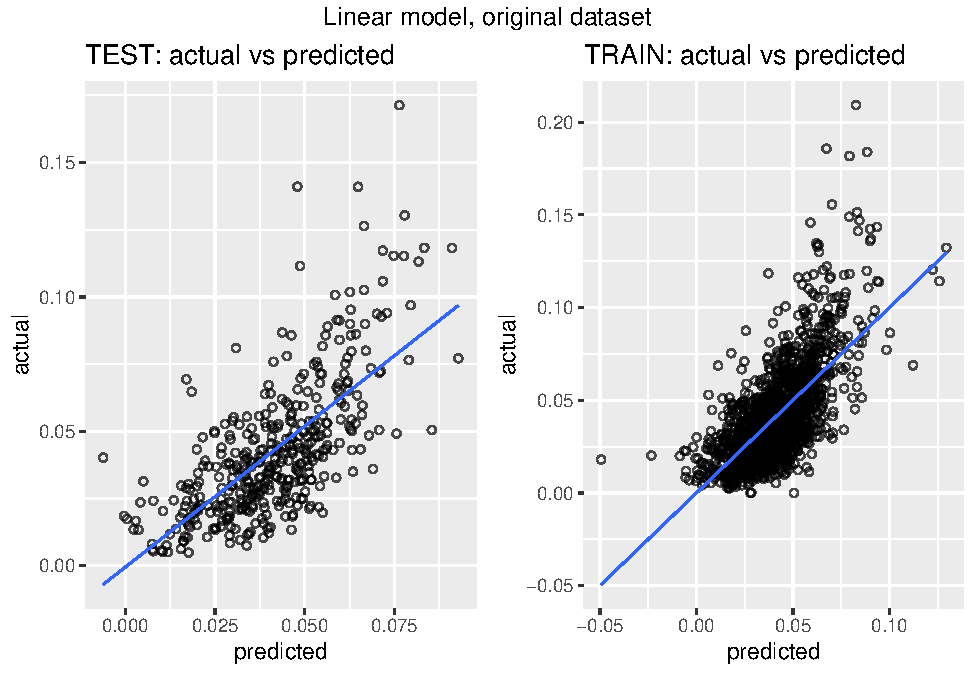
\includegraphics{Lin_Mod_Clus_Analysis_files/figure-latex/unnamed-chunk-31-1.pdf}

\begin{Shaded}
\begin{Highlighting}[]
\CommentTok{\# qplot(d.train$GA\_share, predict.lm(lm1, d.train), colour = d.train$language)}
\CommentTok{\# plot(lm1)}
\end{Highlighting}
\end{Shaded}

Now the same for the GLM:

\begin{Shaded}
\begin{Highlighting}[]
\NormalTok{glmte }\OtherTok{\textless{}{-}} \FunctionTok{ggplot}\NormalTok{(d.test, }\FunctionTok{aes}\NormalTok{(}\AttributeTok{y=}\NormalTok{GA\_share ,}\AttributeTok{x=}\FunctionTok{predict}\NormalTok{(glmodel1, d.test, }\AttributeTok{type=}\StringTok{"response"}\NormalTok{))) }\SpecialCharTok{+}
  \FunctionTok{labs}\NormalTok{(}\AttributeTok{y=} \StringTok{"actual"}\NormalTok{, }\AttributeTok{x =} \StringTok{"predicted"}\NormalTok{) }\SpecialCharTok{+} \FunctionTok{ggtitle}\NormalTok{(}\StringTok{"TEST: actual vs predicted"}\NormalTok{) }\SpecialCharTok{+} 
  \FunctionTok{geom\_point}\NormalTok{(}\AttributeTok{shape =} \DecValTok{1}\NormalTok{, }\AttributeTok{alpha =} \FloatTok{0.7}\NormalTok{)}

\NormalTok{glmtr }\OtherTok{\textless{}{-}} \FunctionTok{ggplot}\NormalTok{(d.train,}\FunctionTok{aes}\NormalTok{(}\AttributeTok{y=}\NormalTok{GA\_share, }\AttributeTok{x=}\FunctionTok{predict}\NormalTok{(glmodel1, d.train, }\AttributeTok{type=}\StringTok{"response"}\NormalTok{))) }\SpecialCharTok{+}
  \FunctionTok{labs}\NormalTok{(}\AttributeTok{y=} \StringTok{"actual"}\NormalTok{, }\AttributeTok{x =} \StringTok{"predicted"}\NormalTok{) }\SpecialCharTok{+} \FunctionTok{ggtitle}\NormalTok{(}\StringTok{"TRAIN: actual vs predicted"}\NormalTok{) }\SpecialCharTok{+} 
  \FunctionTok{geom\_point}\NormalTok{(}\AttributeTok{shape =} \DecValTok{1}\NormalTok{, }\AttributeTok{alpha =} \FloatTok{0.7}\NormalTok{)}

\NormalTok{gridExtra}\SpecialCharTok{::}\FunctionTok{grid.arrange}\NormalTok{(}\AttributeTok{nrow =} \DecValTok{1}\NormalTok{, }\AttributeTok{ncol =} \DecValTok{2}\NormalTok{, }
\NormalTok{                        glmte }\SpecialCharTok{+} \FunctionTok{stat\_smooth}\NormalTok{(}\AttributeTok{size=}\FloatTok{0.5}\NormalTok{, }\AttributeTok{method=}\StringTok{"glm"}\NormalTok{,}\AttributeTok{se=}\ConstantTok{FALSE}\NormalTok{),}
\NormalTok{                        glmtr }\SpecialCharTok{+} \FunctionTok{stat\_smooth}\NormalTok{(}\AttributeTok{size=}\FloatTok{0.5}\NormalTok{, }\AttributeTok{method=}\StringTok{"glm"}\NormalTok{,}\AttributeTok{se=}\ConstantTok{FALSE}\NormalTok{),}
                        \AttributeTok{top=}\StringTok{"GLM Quasibinomial model 1. original dataset"}\NormalTok{)}
\end{Highlighting}
\end{Shaded}

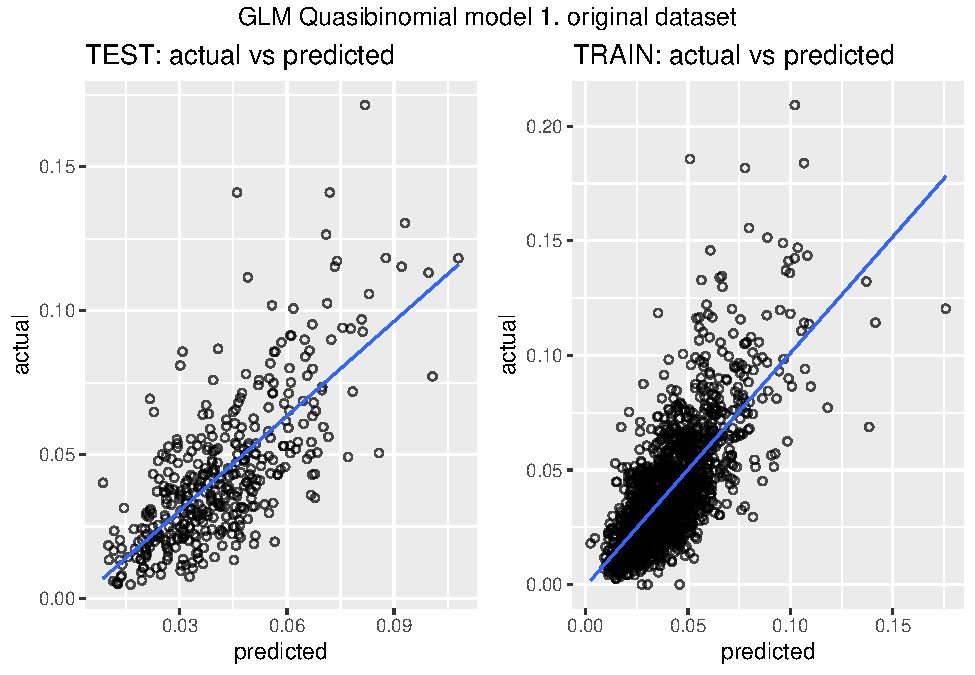
\includegraphics{Lin_Mod_Clus_Analysis_files/figure-latex/unnamed-chunk-32-1.pdf}

\begin{Shaded}
\begin{Highlighting}[]
\CommentTok{\# qplot(d.train$GA\_share, predict(glmodel1, d.train, type="response"), colour = d.train$language)}
\CommentTok{\# plot(glmodel1)}
\end{Highlighting}
\end{Shaded}

Now the same for the GLM 2 :

\begin{Shaded}
\begin{Highlighting}[]
\NormalTok{glmte2 }\OtherTok{\textless{}{-}} \FunctionTok{ggplot}\NormalTok{(d.test, }\FunctionTok{aes}\NormalTok{(}\AttributeTok{y=}\NormalTok{GA\_share ,}\AttributeTok{x=}\FunctionTok{predict}\NormalTok{(glmodel2, d.test, }\AttributeTok{type=}\StringTok{"response"}\NormalTok{))) }\SpecialCharTok{+}
  \FunctionTok{labs}\NormalTok{(}\AttributeTok{y=} \StringTok{"actual"}\NormalTok{, }\AttributeTok{x =} \StringTok{"predicted"}\NormalTok{) }\SpecialCharTok{+} \FunctionTok{ggtitle}\NormalTok{(}\StringTok{"TEST: actual vs predicted"}\NormalTok{) }\SpecialCharTok{+} 
  \FunctionTok{geom\_point}\NormalTok{(}\AttributeTok{shape =} \DecValTok{1}\NormalTok{, }\AttributeTok{alpha =} \FloatTok{0.7}\NormalTok{)}

\NormalTok{glmtr2 }\OtherTok{\textless{}{-}} \FunctionTok{ggplot}\NormalTok{(d.train,}\FunctionTok{aes}\NormalTok{(}\AttributeTok{y=}\NormalTok{GA\_share, }\AttributeTok{x=}\FunctionTok{predict}\NormalTok{(glmodel2, d.train, }\AttributeTok{type=}\StringTok{"response"}\NormalTok{))) }\SpecialCharTok{+}
  \FunctionTok{labs}\NormalTok{(}\AttributeTok{y=} \StringTok{"actual"}\NormalTok{, }\AttributeTok{x =} \StringTok{"predicted"}\NormalTok{) }\SpecialCharTok{+} \FunctionTok{ggtitle}\NormalTok{(}\StringTok{"TRAIN: actual vs predicted"}\NormalTok{) }\SpecialCharTok{+} 
  \FunctionTok{geom\_point}\NormalTok{(}\AttributeTok{shape =} \DecValTok{1}\NormalTok{, }\AttributeTok{alpha =} \FloatTok{0.7}\NormalTok{)}

\NormalTok{gridExtra}\SpecialCharTok{::}\FunctionTok{grid.arrange}\NormalTok{(}\AttributeTok{nrow =} \DecValTok{1}\NormalTok{, }\AttributeTok{ncol =} \DecValTok{2}\NormalTok{, }
\NormalTok{                        glmte2 }\SpecialCharTok{+} \FunctionTok{stat\_smooth}\NormalTok{(}\AttributeTok{size=}\FloatTok{0.5}\NormalTok{, }\AttributeTok{method=}\StringTok{"glm"}\NormalTok{,}\AttributeTok{se=}\ConstantTok{FALSE}\NormalTok{),}
\NormalTok{                        glmtr2 }\SpecialCharTok{+} \FunctionTok{stat\_smooth}\NormalTok{(}\AttributeTok{size=}\FloatTok{0.5}\NormalTok{, }\AttributeTok{method=}\StringTok{"glm"}\NormalTok{,}\AttributeTok{se=}\ConstantTok{FALSE}\NormalTok{),}
                        \AttributeTok{top=}\StringTok{"GLM Quasibinomial model 2, original dataset"}\NormalTok{)}
\end{Highlighting}
\end{Shaded}

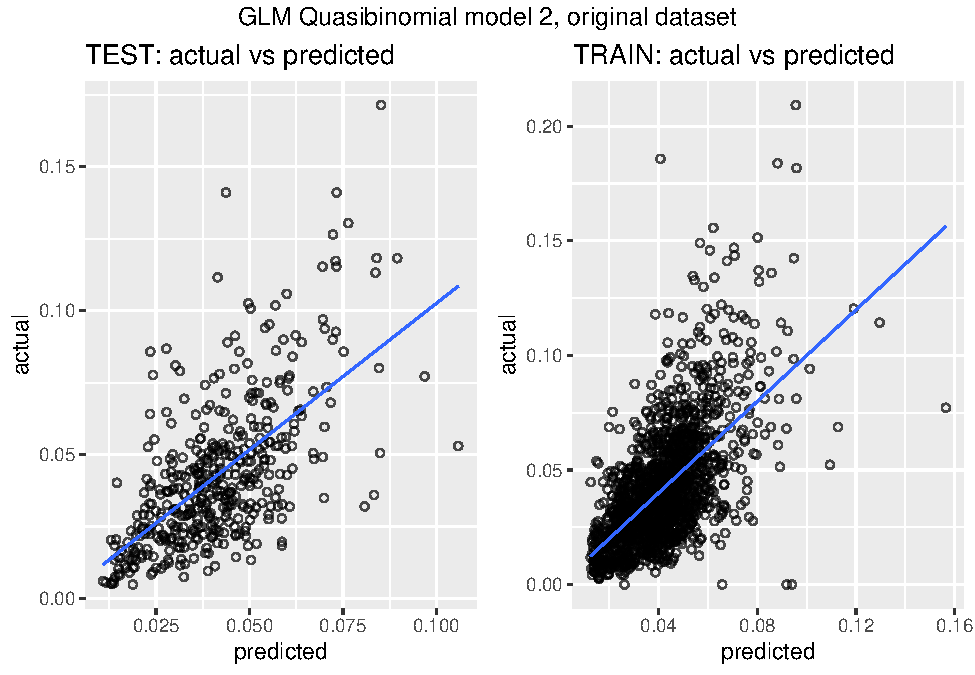
\includegraphics{Lin_Mod_Clus_Analysis_files/figure-latex/unnamed-chunk-33-1.pdf}

\begin{Shaded}
\begin{Highlighting}[]
\CommentTok{\# qplot(d.train$GA\_share, predict(glmodel1, d.train, type="response"), colour = d.train$language)}
\CommentTok{\# plot(glmodel1)}
\end{Highlighting}
\end{Shaded}

Now the whole thing again for the normalized dataset:

First the graphically view, comparing the prediction for Test and Train
data for final linear model:

\begin{Shaded}
\begin{Highlighting}[]
\NormalTok{mte.norm }\OtherTok{\textless{}{-}} \FunctionTok{ggplot}\NormalTok{(d.norm.test, }\FunctionTok{aes}\NormalTok{(}\AttributeTok{y=}\NormalTok{GA\_share ,}\AttributeTok{x=}\FunctionTok{predict}\NormalTok{(lm.norm}\FloatTok{.1}\NormalTok{, d.norm.test))) }\SpecialCharTok{+}
  \FunctionTok{labs}\NormalTok{(}\AttributeTok{y=} \StringTok{"actual"}\NormalTok{, }\AttributeTok{x =} \StringTok{"predicted"}\NormalTok{) }\SpecialCharTok{+} \FunctionTok{ggtitle}\NormalTok{(}\StringTok{"TEST: actual vs predicted"}\NormalTok{) }\SpecialCharTok{+} 
  \FunctionTok{geom\_point}\NormalTok{(}\AttributeTok{shape =} \DecValTok{1}\NormalTok{, }\AttributeTok{alpha =} \FloatTok{0.7}\NormalTok{)}

\NormalTok{mtr.norm }\OtherTok{\textless{}{-}} \FunctionTok{ggplot}\NormalTok{(d.norm.train,}\FunctionTok{aes}\NormalTok{(}\AttributeTok{y=}\NormalTok{GA\_share, }\AttributeTok{x=}\FunctionTok{predict}\NormalTok{(lm.norm}\FloatTok{.1}\NormalTok{, d.norm.train))) }\SpecialCharTok{+}
  \FunctionTok{labs}\NormalTok{(}\AttributeTok{y=} \StringTok{"actual"}\NormalTok{, }\AttributeTok{x =} \StringTok{"predicted"}\NormalTok{) }\SpecialCharTok{+} \FunctionTok{ggtitle}\NormalTok{(}\StringTok{"TRAIN: actual vs predicted"}\NormalTok{) }\SpecialCharTok{+} 
  \FunctionTok{geom\_point}\NormalTok{(}\AttributeTok{shape =} \DecValTok{1}\NormalTok{, }\AttributeTok{alpha =} \FloatTok{0.7}\NormalTok{)}

\NormalTok{gridExtra}\SpecialCharTok{::}\FunctionTok{grid.arrange}\NormalTok{(}\AttributeTok{nrow =} \DecValTok{1}\NormalTok{, }\AttributeTok{ncol =} \DecValTok{2}\NormalTok{, mte.norm }\SpecialCharTok{+} 
                        \FunctionTok{stat\_smooth}\NormalTok{(}\AttributeTok{size=}\FloatTok{0.5}\NormalTok{, }\AttributeTok{method=}\StringTok{"lm"}\NormalTok{,}\AttributeTok{se=}\ConstantTok{FALSE}\NormalTok{), }
\NormalTok{                        mtr.norm }\SpecialCharTok{+} \FunctionTok{stat\_smooth}\NormalTok{(}\AttributeTok{size=}\FloatTok{0.5}\NormalTok{, }\AttributeTok{method=}\StringTok{"lm"}\NormalTok{,}\AttributeTok{se=}\ConstantTok{FALSE}\NormalTok{),}
                        \AttributeTok{top =} \StringTok{"Linear model, Normalized dataset"}\NormalTok{)}
\end{Highlighting}
\end{Shaded}

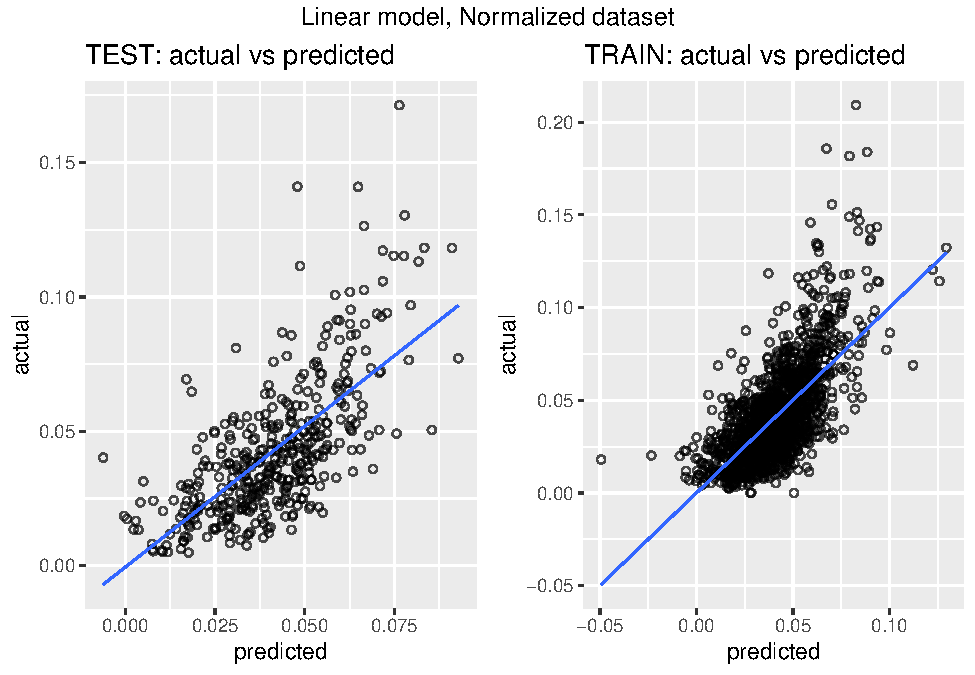
\includegraphics{Lin_Mod_Clus_Analysis_files/figure-latex/unnamed-chunk-34-1.pdf}

\begin{Shaded}
\begin{Highlighting}[]
\CommentTok{\# qplot(d.train$GA\_share, predict.lm(lm1, d.train), colour = d.train$language)}
\CommentTok{\# plot(lm1)}
\end{Highlighting}
\end{Shaded}

Now the same for the GLM:

\begin{Shaded}
\begin{Highlighting}[]
\NormalTok{glmte.norm }\OtherTok{\textless{}{-}} \FunctionTok{ggplot}\NormalTok{(d.norm.test, }\FunctionTok{aes}\NormalTok{(}\AttributeTok{y=}\NormalTok{GA\_share ,}\AttributeTok{x=}\FunctionTok{predict}\NormalTok{(glmodel.norm}\FloatTok{.1}\NormalTok{, d.norm.test, }\AttributeTok{type=}\StringTok{"response"}\NormalTok{))) }\SpecialCharTok{+}
  \FunctionTok{labs}\NormalTok{(}\AttributeTok{y=} \StringTok{"actual"}\NormalTok{, }\AttributeTok{x =} \StringTok{"predicted"}\NormalTok{) }\SpecialCharTok{+} \FunctionTok{ggtitle}\NormalTok{(}\StringTok{"TEST: actual vs predicted"}\NormalTok{) }\SpecialCharTok{+} 
  \FunctionTok{geom\_point}\NormalTok{(}\AttributeTok{shape =} \DecValTok{1}\NormalTok{, }\AttributeTok{alpha =} \FloatTok{0.7}\NormalTok{)}

\NormalTok{glmtr.norm }\OtherTok{\textless{}{-}} \FunctionTok{ggplot}\NormalTok{(d.norm.train,}\FunctionTok{aes}\NormalTok{(}\AttributeTok{y=}\NormalTok{GA\_share, }\AttributeTok{x=}\FunctionTok{predict}\NormalTok{(glmodel.norm}\FloatTok{.1}\NormalTok{, d.norm.train, }\AttributeTok{type=}\StringTok{"response"}\NormalTok{))) }\SpecialCharTok{+}
  \FunctionTok{labs}\NormalTok{(}\AttributeTok{y=} \StringTok{"actual"}\NormalTok{, }\AttributeTok{x =} \StringTok{"predicted"}\NormalTok{) }\SpecialCharTok{+} \FunctionTok{ggtitle}\NormalTok{(}\StringTok{"TRAIN: actual vs predicted"}\NormalTok{) }\SpecialCharTok{+} 
  \FunctionTok{geom\_point}\NormalTok{(}\AttributeTok{shape =} \DecValTok{1}\NormalTok{, }\AttributeTok{alpha =} \FloatTok{0.7}\NormalTok{)}

\NormalTok{gridExtra}\SpecialCharTok{::}\FunctionTok{grid.arrange}\NormalTok{(}\AttributeTok{nrow =} \DecValTok{1}\NormalTok{, }\AttributeTok{ncol =} \DecValTok{2}\NormalTok{, }
\NormalTok{                        glmte.norm }\SpecialCharTok{+} \FunctionTok{stat\_smooth}\NormalTok{(}\AttributeTok{size=}\FloatTok{0.5}\NormalTok{, }\AttributeTok{method=}\StringTok{"glm"}\NormalTok{,}\AttributeTok{se=}\ConstantTok{FALSE}\NormalTok{),}
\NormalTok{                        glmtr.norm }\SpecialCharTok{+} \FunctionTok{stat\_smooth}\NormalTok{(}\AttributeTok{size=}\FloatTok{0.5}\NormalTok{, }\AttributeTok{method=}\StringTok{"glm"}\NormalTok{,}\AttributeTok{se=}\ConstantTok{FALSE}\NormalTok{),}
                        \AttributeTok{top=}\StringTok{"GLM Quasibinomial model 1, Normalized dataset"}\NormalTok{)}
\end{Highlighting}
\end{Shaded}

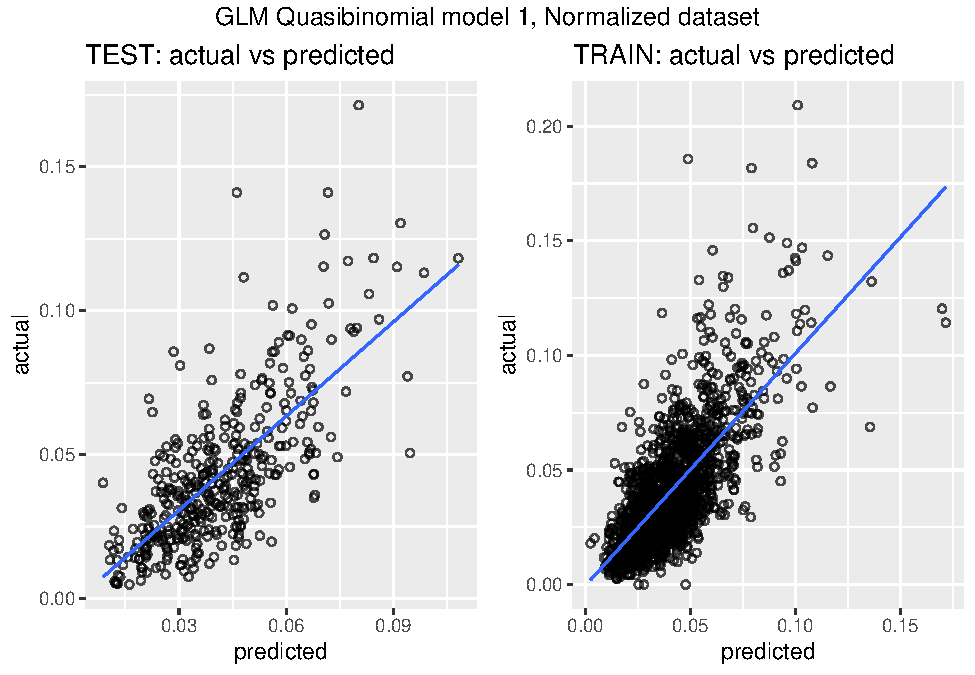
\includegraphics{Lin_Mod_Clus_Analysis_files/figure-latex/unnamed-chunk-35-1.pdf}

\begin{Shaded}
\begin{Highlighting}[]
\CommentTok{\# qplot(d.train$GA\_share, predict(glmodel1, d.train, type="response"), colour = d.train$language)}
\CommentTok{\# plot(glmodel1)}
\end{Highlighting}
\end{Shaded}

Now the same for the GLM 2 :

\begin{Shaded}
\begin{Highlighting}[]
\NormalTok{glmte.norm}\FloatTok{.2} \OtherTok{\textless{}{-}} \FunctionTok{ggplot}\NormalTok{(d.norm.test, }\FunctionTok{aes}\NormalTok{(}\AttributeTok{y=}\NormalTok{GA\_share ,}\AttributeTok{x=}\FunctionTok{predict}\NormalTok{(glmodel.norm}\FloatTok{.2}\NormalTok{, d.norm.test, }\AttributeTok{type=}\StringTok{"response"}\NormalTok{))) }\SpecialCharTok{+}
  \FunctionTok{labs}\NormalTok{(}\AttributeTok{y=} \StringTok{"actual"}\NormalTok{, }\AttributeTok{x =} \StringTok{"predicted"}\NormalTok{) }\SpecialCharTok{+} \FunctionTok{ggtitle}\NormalTok{(}\StringTok{"TEST: actual vs predicted"}\NormalTok{) }\SpecialCharTok{+} 
  \FunctionTok{geom\_point}\NormalTok{(}\AttributeTok{shape =} \DecValTok{1}\NormalTok{, }\AttributeTok{alpha =} \FloatTok{0.7}\NormalTok{)}

\NormalTok{glmtr.norm}\FloatTok{.2} \OtherTok{\textless{}{-}} \FunctionTok{ggplot}\NormalTok{(d.norm.train,}\FunctionTok{aes}\NormalTok{(}\AttributeTok{y=}\NormalTok{GA\_share, }\AttributeTok{x=}\FunctionTok{predict}\NormalTok{(glmodel.norm}\FloatTok{.2}\NormalTok{, d.norm.train, }\AttributeTok{type=}\StringTok{"response"}\NormalTok{))) }\SpecialCharTok{+}
  \FunctionTok{labs}\NormalTok{(}\AttributeTok{y=} \StringTok{"actual"}\NormalTok{, }\AttributeTok{x =} \StringTok{"predicted"}\NormalTok{) }\SpecialCharTok{+} \FunctionTok{ggtitle}\NormalTok{(}\StringTok{"TRAIN: actual vs predicted"}\NormalTok{) }\SpecialCharTok{+} 
  \FunctionTok{geom\_point}\NormalTok{(}\AttributeTok{shape =} \DecValTok{1}\NormalTok{, }\AttributeTok{alpha =} \FloatTok{0.7}\NormalTok{)}

\NormalTok{gridExtra}\SpecialCharTok{::}\FunctionTok{grid.arrange}\NormalTok{(}\AttributeTok{nrow =} \DecValTok{1}\NormalTok{, }\AttributeTok{ncol =} \DecValTok{2}\NormalTok{, }
\NormalTok{                        glmte.norm}\FloatTok{.2} \SpecialCharTok{+} \FunctionTok{stat\_smooth}\NormalTok{(}\AttributeTok{size=}\FloatTok{0.5}\NormalTok{, }\AttributeTok{method=}\StringTok{"glm"}\NormalTok{,}\AttributeTok{se=}\ConstantTok{FALSE}\NormalTok{),}
\NormalTok{                        glmtr.norm}\FloatTok{.2} \SpecialCharTok{+} \FunctionTok{stat\_smooth}\NormalTok{(}\AttributeTok{size=}\FloatTok{0.5}\NormalTok{, }\AttributeTok{method=}\StringTok{"glm"}\NormalTok{,}\AttributeTok{se=}\ConstantTok{FALSE}\NormalTok{),}
                        \AttributeTok{top=}\StringTok{"GLM Quasibinomial model 2, original dataset"}\NormalTok{)}
\end{Highlighting}
\end{Shaded}

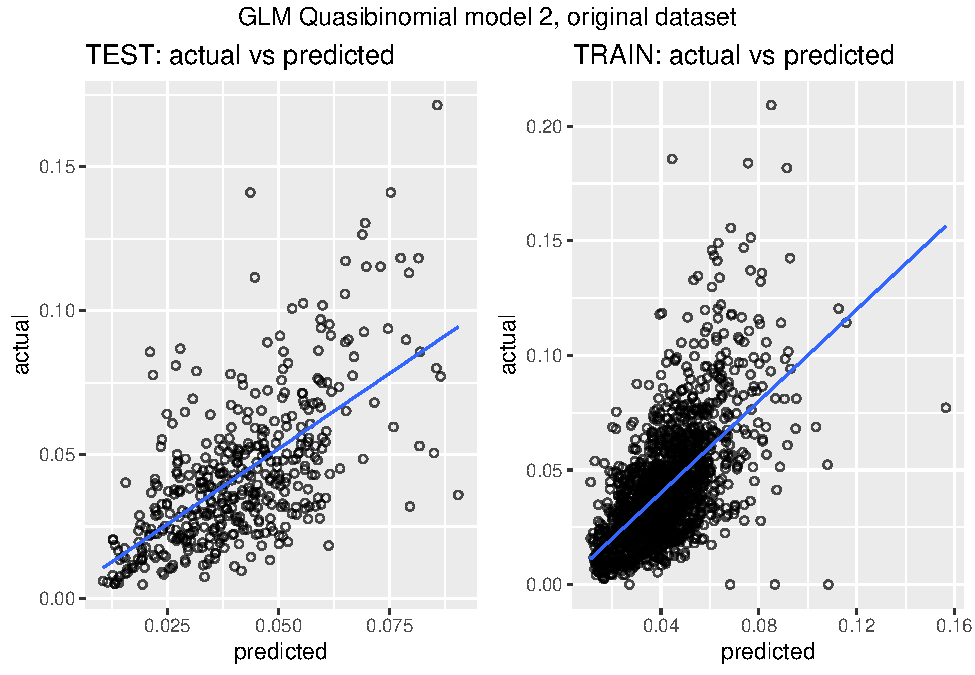
\includegraphics{Lin_Mod_Clus_Analysis_files/figure-latex/unnamed-chunk-36-1.pdf}

\begin{Shaded}
\begin{Highlighting}[]
\CommentTok{\# qplot(d.train$GA\_share, predict(glmodel1, d.train, type="response"), colour = d.train$language)}
\CommentTok{\# plot(glmodel1)}
\end{Highlighting}
\end{Shaded}

\hypertarget{evaluation-results}{%
\subsubsection{Evaluation results}\label{evaluation-results}}

\hypertarget{original-dataset-1}{%
\paragraph{Original dataset}\label{original-dataset-1}}

Now the comparison of the RMSE and Rsquare values:

First the values for the linear model, which takes all variables into
account:

\begin{Shaded}
\begin{Highlighting}[]
\NormalTok{lm0.eval.train }\OtherTok{\textless{}{-}} \FunctionTok{eval\_results}\NormalTok{(d.train}\SpecialCharTok{$}\NormalTok{GA\_share, }\FunctionTok{predict.lm}\NormalTok{(lm0, d.train))}
\NormalTok{lm0.eval.test }\OtherTok{\textless{}{-}} \FunctionTok{eval\_results}\NormalTok{(d.test}\SpecialCharTok{$}\NormalTok{GA\_share, }\FunctionTok{predict.lm}\NormalTok{(lm0, d.test))}

\FunctionTok{writeLines}\NormalTok{(}\FunctionTok{paste}\NormalTok{(}\StringTok{"Lm0: RMSE train: "}\NormalTok{, }\FunctionTok{round}\NormalTok{(lm0.eval.train}\SpecialCharTok{$}\NormalTok{RMSE, }\DecValTok{4}\NormalTok{),}
                 \StringTok{"}\SpecialCharTok{\textbackslash{}n}\StringTok{Lm0: Rsquare train: "}\NormalTok{,}\FunctionTok{round}\NormalTok{(lm0.eval.train}\SpecialCharTok{$}\NormalTok{Rsquare, }\DecValTok{3}\NormalTok{),}
                 \StringTok{"}\SpecialCharTok{\textbackslash{}n}\StringTok{Lm0: RMSE test: "}\NormalTok{, }\FunctionTok{round}\NormalTok{(lm0.eval.test}\SpecialCharTok{$}\NormalTok{RMSE, }\DecValTok{4}\NormalTok{),}
                 \StringTok{"}\SpecialCharTok{\textbackslash{}n}\StringTok{Lm0: Rsquare test: "}\NormalTok{, }\FunctionTok{round}\NormalTok{(lm0.eval.test}\SpecialCharTok{$}\NormalTok{Rsquare, }\DecValTok{3}\NormalTok{)))}
\end{Highlighting}
\end{Shaded}

\begin{verbatim}
## Lm0: RMSE train:  0.0179 
## Lm0: Rsquare train:  0.506 
## Lm0: RMSE test:  0.0179 
## Lm0: Rsquare test:  0.51
\end{verbatim}

\begin{Shaded}
\begin{Highlighting}[]
\CommentTok{\# qplot(d.train$GA\_share, predict.lm(lm0, d.train), colour = d.train$language)}
\end{Highlighting}
\end{Shaded}

Second, the values for the linear model, which takes only selected
variables into account:

\begin{Shaded}
\begin{Highlighting}[]
\NormalTok{lm1.eval.train }\OtherTok{\textless{}{-}} \FunctionTok{eval\_results}\NormalTok{(d.train}\SpecialCharTok{$}\NormalTok{GA\_share, }\FunctionTok{predict.lm}\NormalTok{(lm1, d.train)) }
\NormalTok{lm1.eval.test }\OtherTok{\textless{}{-}} \FunctionTok{eval\_results}\NormalTok{(d.test}\SpecialCharTok{$}\NormalTok{GA\_share, }\FunctionTok{predict.lm}\NormalTok{(lm1, d.test))}

\FunctionTok{writeLines}\NormalTok{(}\FunctionTok{paste}\NormalTok{(}\StringTok{"Lm1: RMSE train: "}\NormalTok{, }\FunctionTok{round}\NormalTok{(lm1.eval.train}\SpecialCharTok{$}\NormalTok{RMSE, }\DecValTok{4}\NormalTok{), }
                 \StringTok{"}\SpecialCharTok{\textbackslash{}n}\StringTok{Lm1: Rsquare train: "}\NormalTok{,}\FunctionTok{round}\NormalTok{(lm1.eval.train}\SpecialCharTok{$}\NormalTok{Rsquare, }\DecValTok{3}\NormalTok{), }
                 \StringTok{"}\SpecialCharTok{\textbackslash{}n}\StringTok{Lm1: RMSE test: "}\NormalTok{, }\FunctionTok{round}\NormalTok{(lm1.eval.test}\SpecialCharTok{$}\NormalTok{RMSE, }\DecValTok{4}\NormalTok{), }
                 \StringTok{"}\SpecialCharTok{\textbackslash{}n}\StringTok{Lm1: Rsquare test: "}\NormalTok{, }\FunctionTok{round}\NormalTok{(lm1.eval.test}\SpecialCharTok{$}\NormalTok{Rsquare, }\DecValTok{3}\NormalTok{)))}
\end{Highlighting}
\end{Shaded}

\begin{verbatim}
## Lm1: RMSE train:  0.0179 
## Lm1: Rsquare train:  0.505 
## Lm1: RMSE test:  0.018 
## Lm1: Rsquare test:  0.508
\end{verbatim}

And second the values for the GLM:

\begin{Shaded}
\begin{Highlighting}[]
\NormalTok{glmodel0.eval.train }\OtherTok{\textless{}{-}} \FunctionTok{eval\_results}\NormalTok{(d.train[,}\DecValTok{4}\SpecialCharTok{:}\DecValTok{50}\NormalTok{]}\SpecialCharTok{$}\NormalTok{GA\_share, }\FunctionTok{predict}\NormalTok{(glmodel0, d.train[,}\DecValTok{4}\SpecialCharTok{:}\DecValTok{50}\NormalTok{], }\AttributeTok{type=}\StringTok{"response"}\NormalTok{)) }
\NormalTok{glmodel0.eval.test }\OtherTok{\textless{}{-}} \FunctionTok{eval\_results}\NormalTok{(d.test[,}\DecValTok{4}\SpecialCharTok{:}\DecValTok{50}\NormalTok{]}\SpecialCharTok{$}\NormalTok{GA\_share, }\FunctionTok{predict}\NormalTok{(glmodel0, d.test[,}\DecValTok{4}\SpecialCharTok{:}\DecValTok{50}\NormalTok{], }\AttributeTok{type=}\StringTok{"response"}\NormalTok{))}

\FunctionTok{writeLines}\NormalTok{(}\FunctionTok{paste}\NormalTok{(}\StringTok{"GLM0: RMSE train: "}\NormalTok{, }\FunctionTok{round}\NormalTok{(glmodel0.eval.train}\SpecialCharTok{$}\NormalTok{RMSE, }\DecValTok{5}\NormalTok{), }
                 \StringTok{"}\SpecialCharTok{\textbackslash{}n}\StringTok{GLM0: Rsquare train: "}\NormalTok{,}\FunctionTok{round}\NormalTok{(glmodel0.eval.train}\SpecialCharTok{$}\NormalTok{Rsquare, }\DecValTok{3}\NormalTok{),}
                 \StringTok{"}\SpecialCharTok{\textbackslash{}n}\StringTok{GLM0: RMSE test: "}\NormalTok{, }\FunctionTok{round}\NormalTok{(glmodel0.eval.test}\SpecialCharTok{$}\NormalTok{RMSE, }\DecValTok{5}\NormalTok{), }
                 \StringTok{"}\SpecialCharTok{\textbackslash{}n}\StringTok{GLM0: Rsquare test: "}\NormalTok{, }\FunctionTok{round}\NormalTok{(glmodel0.eval.test}\SpecialCharTok{$}\NormalTok{Rsquare, }\DecValTok{3}\NormalTok{)))}
\end{Highlighting}
\end{Shaded}

\begin{verbatim}
## GLM0: RMSE train:  0.01702 
## GLM0: Rsquare train:  0.553 
## GLM0: RMSE test:  0.01703 
## GLM0: Rsquare test:  0.558
\end{verbatim}

\begin{Shaded}
\begin{Highlighting}[]
\NormalTok{glmodel1.eval.train }\OtherTok{\textless{}{-}} \FunctionTok{eval\_results}\NormalTok{(d.train[,}\DecValTok{4}\SpecialCharTok{:}\DecValTok{50}\NormalTok{]}\SpecialCharTok{$}\NormalTok{GA\_share, }\FunctionTok{predict}\NormalTok{(glmodel1, d.train[,}\DecValTok{4}\SpecialCharTok{:}\DecValTok{50}\NormalTok{], }\AttributeTok{type=}\StringTok{"response"}\NormalTok{)) }
\NormalTok{glmodel1.eval.test }\OtherTok{\textless{}{-}} \FunctionTok{eval\_results}\NormalTok{(d.test[,}\DecValTok{4}\SpecialCharTok{:}\DecValTok{50}\NormalTok{]}\SpecialCharTok{$}\NormalTok{GA\_share, }\FunctionTok{predict}\NormalTok{(glmodel1, d.test[,}\DecValTok{4}\SpecialCharTok{:}\DecValTok{50}\NormalTok{], }\AttributeTok{type=}\StringTok{"response"}\NormalTok{))}

\FunctionTok{writeLines}\NormalTok{(}\FunctionTok{paste}\NormalTok{(}\StringTok{"GLM1: RMSE train: "}\NormalTok{, }\FunctionTok{round}\NormalTok{(glmodel1.eval.train}\SpecialCharTok{$}\NormalTok{RMSE, }\DecValTok{5}\NormalTok{), }
                 \StringTok{"}\SpecialCharTok{\textbackslash{}n}\StringTok{GLM1: Rsquare train: "}\NormalTok{,}\FunctionTok{round}\NormalTok{(glmodel1.eval.train}\SpecialCharTok{$}\NormalTok{Rsquare, }\DecValTok{3}\NormalTok{),}
                 \StringTok{"}\SpecialCharTok{\textbackslash{}n}\StringTok{GLM1: RMSE test: "}\NormalTok{, }\FunctionTok{round}\NormalTok{(glmodel1.eval.test}\SpecialCharTok{$}\NormalTok{RMSE, }\DecValTok{5}\NormalTok{), }
                 \StringTok{"}\SpecialCharTok{\textbackslash{}n}\StringTok{GLM1: Rsquare test: "}\NormalTok{, }\FunctionTok{round}\NormalTok{(glmodel1.eval.test}\SpecialCharTok{$}\NormalTok{Rsquare, }\DecValTok{3}\NormalTok{)))}
\end{Highlighting}
\end{Shaded}

\begin{verbatim}
## GLM1: RMSE train:  0.01712 
## GLM1: Rsquare train:  0.548 
## GLM1: RMSE test:  0.01705 
## GLM1: Rsquare test:  0.557
\end{verbatim}

\begin{Shaded}
\begin{Highlighting}[]
\NormalTok{glmodel2.eval.train }\OtherTok{\textless{}{-}} \FunctionTok{eval\_results}\NormalTok{(d.train[,}\DecValTok{4}\SpecialCharTok{:}\DecValTok{50}\NormalTok{]}\SpecialCharTok{$}\NormalTok{GA\_share, }\FunctionTok{predict}\NormalTok{(glmodel2, d.train[,}\DecValTok{4}\SpecialCharTok{:}\DecValTok{50}\NormalTok{], }\AttributeTok{type=}\StringTok{"response"}\NormalTok{)) }
\NormalTok{glmodel2.eval.test }\OtherTok{\textless{}{-}} \FunctionTok{eval\_results}\NormalTok{(d.test[,}\DecValTok{4}\SpecialCharTok{:}\DecValTok{50}\NormalTok{]}\SpecialCharTok{$}\NormalTok{GA\_share, }\FunctionTok{predict}\NormalTok{(glmodel2, d.test[,}\DecValTok{4}\SpecialCharTok{:}\DecValTok{50}\NormalTok{], }\AttributeTok{type=}\StringTok{"response"}\NormalTok{))}

\FunctionTok{writeLines}\NormalTok{(}\FunctionTok{paste}\NormalTok{(}\StringTok{"GLM2: RMSE train: "}\NormalTok{, }\FunctionTok{round}\NormalTok{(glmodel2.eval.train}\SpecialCharTok{$}\NormalTok{RMSE, }\DecValTok{4}\NormalTok{), }
                 \StringTok{"}\SpecialCharTok{\textbackslash{}n}\StringTok{GLM2: Rsquare train: "}\NormalTok{,}\FunctionTok{round}\NormalTok{(glmodel2.eval.train}\SpecialCharTok{$}\NormalTok{Rsquare, }\DecValTok{3}\NormalTok{),}
                 \StringTok{"}\SpecialCharTok{\textbackslash{}n}\StringTok{GLM2: RMSE test: "}\NormalTok{, }\FunctionTok{round}\NormalTok{(glmodel2.eval.test}\SpecialCharTok{$}\NormalTok{RMSE, }\DecValTok{4}\NormalTok{), }
                 \StringTok{"}\SpecialCharTok{\textbackslash{}n}\StringTok{GLM2: Rsquare test: "}\NormalTok{, }\FunctionTok{round}\NormalTok{(glmodel2.eval.test}\SpecialCharTok{$}\NormalTok{Rsquare, }\DecValTok{3}\NormalTok{)))}
\end{Highlighting}
\end{Shaded}

\begin{verbatim}
## GLM2: RMSE train:  0.0196 
## GLM2: Rsquare train:  0.408 
## GLM2: RMSE test:  0.0198 
## GLM2: Rsquare test:  0.403
\end{verbatim}

\hypertarget{normalized-dataset-1}{%
\paragraph{Normalized dataset}\label{normalized-dataset-1}}

Now the comparison of the RMSE and Rsquare values:

First the values for the linear model, which takes all variables into
account:

\begin{Shaded}
\begin{Highlighting}[]
\NormalTok{lm.norm.}\FloatTok{0.}\NormalTok{eval.train }\OtherTok{\textless{}{-}} \FunctionTok{eval\_results}\NormalTok{(d.norm.train}\SpecialCharTok{$}\NormalTok{GA\_share, }\FunctionTok{predict.lm}\NormalTok{(lm.norm}\FloatTok{.0}\NormalTok{, d.norm.train))}
\NormalTok{lm.norm.}\FloatTok{0.}\NormalTok{eval.test }\OtherTok{\textless{}{-}} \FunctionTok{eval\_results}\NormalTok{(d.norm.test}\SpecialCharTok{$}\NormalTok{GA\_share, }\FunctionTok{predict.lm}\NormalTok{(lm.norm}\FloatTok{.0}\NormalTok{, d.norm.test))}

\FunctionTok{writeLines}\NormalTok{(}\FunctionTok{paste}\NormalTok{(}\StringTok{"Lm.norm.0: RMSE train: "}\NormalTok{, }\FunctionTok{round}\NormalTok{(lm.norm.}\FloatTok{0.}\NormalTok{eval.train}\SpecialCharTok{$}\NormalTok{RMSE, }\DecValTok{4}\NormalTok{),}
                 \StringTok{"}\SpecialCharTok{\textbackslash{}n}\StringTok{Lm.norm.0: Rsquare train: "}\NormalTok{,}\FunctionTok{round}\NormalTok{(lm.norm.}\FloatTok{0.}\NormalTok{eval.train}\SpecialCharTok{$}\NormalTok{Rsquare, }\DecValTok{3}\NormalTok{),}
                 \StringTok{"}\SpecialCharTok{\textbackslash{}n}\StringTok{Lm.norm.0: RMSE test: "}\NormalTok{, }\FunctionTok{round}\NormalTok{(lm.norm.}\FloatTok{0.}\NormalTok{eval.test}\SpecialCharTok{$}\NormalTok{RMSE, }\DecValTok{4}\NormalTok{),}
                 \StringTok{"}\SpecialCharTok{\textbackslash{}n}\StringTok{Lm.norm.0: Rsquare test: "}\NormalTok{, }\FunctionTok{round}\NormalTok{(lm.norm.}\FloatTok{0.}\NormalTok{eval.test}\SpecialCharTok{$}\NormalTok{Rsquare, }\DecValTok{3}\NormalTok{)))}
\end{Highlighting}
\end{Shaded}

\begin{verbatim}
## Lm.norm.0: RMSE train:  0.0179 
## Lm.norm.0: Rsquare train:  0.506 
## Lm.norm.0: RMSE test:  0.0179 
## Lm.norm.0: Rsquare test:  0.51
\end{verbatim}

Second, the values for the linear model, which takes only selected
variables into account:

\begin{Shaded}
\begin{Highlighting}[]
\NormalTok{lm.norm.}\FloatTok{1.}\NormalTok{eval.train }\OtherTok{\textless{}{-}} \FunctionTok{eval\_results}\NormalTok{(d.norm.train}\SpecialCharTok{$}\NormalTok{GA\_share, }\FunctionTok{predict.lm}\NormalTok{(lm.norm}\FloatTok{.1}\NormalTok{, d.norm.train))}
\NormalTok{lm.norm.}\FloatTok{1.}\NormalTok{eval.test }\OtherTok{\textless{}{-}} \FunctionTok{eval\_results}\NormalTok{(d.norm.test}\SpecialCharTok{$}\NormalTok{GA\_share, }\FunctionTok{predict.lm}\NormalTok{(lm.norm}\FloatTok{.1}\NormalTok{, d.norm.test))}

\FunctionTok{writeLines}\NormalTok{(}\FunctionTok{paste}\NormalTok{(}\StringTok{"Lm.norm.1: RMSE train: "}\NormalTok{, }\FunctionTok{round}\NormalTok{(lm.norm.}\FloatTok{1.}\NormalTok{eval.train}\SpecialCharTok{$}\NormalTok{RMSE, }\DecValTok{4}\NormalTok{),}
                 \StringTok{"}\SpecialCharTok{\textbackslash{}n}\StringTok{Lm.norm.1: Rsquare train: "}\NormalTok{,}\FunctionTok{round}\NormalTok{(lm.norm.}\FloatTok{1.}\NormalTok{eval.train}\SpecialCharTok{$}\NormalTok{Rsquare, }\DecValTok{3}\NormalTok{),}
                 \StringTok{"}\SpecialCharTok{\textbackslash{}n}\StringTok{Lm.norm.1: RMSE test: "}\NormalTok{, }\FunctionTok{round}\NormalTok{(lm.norm.}\FloatTok{1.}\NormalTok{eval.test}\SpecialCharTok{$}\NormalTok{RMSE, }\DecValTok{4}\NormalTok{),}
                 \StringTok{"}\SpecialCharTok{\textbackslash{}n}\StringTok{Lm.norm.1: Rsquare test: "}\NormalTok{, }\FunctionTok{round}\NormalTok{(lm.norm.}\FloatTok{1.}\NormalTok{eval.test}\SpecialCharTok{$}\NormalTok{Rsquare, }\DecValTok{3}\NormalTok{)))}
\end{Highlighting}
\end{Shaded}

\begin{verbatim}
## Lm.norm.1: RMSE train:  0.0179 
## Lm.norm.1: Rsquare train:  0.505 
## Lm.norm.1: RMSE test:  0.018 
## Lm.norm.1: Rsquare test:  0.508
\end{verbatim}

And second the values for the GLM:

\begin{Shaded}
\begin{Highlighting}[]
\NormalTok{glmodel.norm.}\FloatTok{0.}\NormalTok{eval.train }\OtherTok{\textless{}{-}} \FunctionTok{eval\_results}\NormalTok{(d.norm.train}\SpecialCharTok{$}\NormalTok{GA\_share, }\FunctionTok{predict}\NormalTok{(glmodel.norm}\FloatTok{.0}\NormalTok{, d.norm.train, }\AttributeTok{type=}\StringTok{"response"}\NormalTok{)) }
\NormalTok{glmodel.norm.}\FloatTok{0.}\NormalTok{eval.test }\OtherTok{\textless{}{-}} \FunctionTok{eval\_results}\NormalTok{(d.norm.test}\SpecialCharTok{$}\NormalTok{GA\_share, }\FunctionTok{predict}\NormalTok{(glmodel.norm}\FloatTok{.0}\NormalTok{, d.norm.test, }\AttributeTok{type=}\StringTok{"response"}\NormalTok{))}

\FunctionTok{writeLines}\NormalTok{(}\FunctionTok{paste}\NormalTok{(}\StringTok{"GLM.norm.0: RMSE train: "}\NormalTok{, }\FunctionTok{round}\NormalTok{(glmodel.norm.}\FloatTok{0.}\NormalTok{eval.train}\SpecialCharTok{$}\NormalTok{RMSE, }\DecValTok{5}\NormalTok{), }
                 \StringTok{"}\SpecialCharTok{\textbackslash{}n}\StringTok{GLM.norm.0: Rsquare train: "}\NormalTok{,}\FunctionTok{round}\NormalTok{(glmodel.norm.}\FloatTok{0.}\NormalTok{eval.train}\SpecialCharTok{$}\NormalTok{Rsquare, }\DecValTok{3}\NormalTok{),}
                 \StringTok{"}\SpecialCharTok{\textbackslash{}n}\StringTok{GLM.norm.0: RMSE test: "}\NormalTok{, }\FunctionTok{round}\NormalTok{(glmodel.norm.}\FloatTok{0.}\NormalTok{eval.test}\SpecialCharTok{$}\NormalTok{RMSE, }\DecValTok{5}\NormalTok{), }
                 \StringTok{"}\SpecialCharTok{\textbackslash{}n}\StringTok{GLM.norm.0: Rsquare test: "}\NormalTok{, }\FunctionTok{round}\NormalTok{(glmodel.norm.}\FloatTok{0.}\NormalTok{eval.test}\SpecialCharTok{$}\NormalTok{Rsquare, }\DecValTok{3}\NormalTok{)))}
\end{Highlighting}
\end{Shaded}

\begin{verbatim}
## GLM.norm.0: RMSE train:  0.01702 
## GLM.norm.0: Rsquare train:  0.553 
## GLM.norm.0: RMSE test:  0.01703 
## GLM.norm.0: Rsquare test:  0.558
\end{verbatim}

\begin{Shaded}
\begin{Highlighting}[]
\NormalTok{glmodel.norm.}\FloatTok{1.}\NormalTok{eval.train }\OtherTok{\textless{}{-}} \FunctionTok{eval\_results}\NormalTok{(d.norm.train}\SpecialCharTok{$}\NormalTok{GA\_share, }\FunctionTok{predict}\NormalTok{(glmodel.norm}\FloatTok{.1}\NormalTok{, d.norm.train, }\AttributeTok{type=}\StringTok{"response"}\NormalTok{)) }
\NormalTok{glmodel.norm.}\FloatTok{1.}\NormalTok{eval.test }\OtherTok{\textless{}{-}} \FunctionTok{eval\_results}\NormalTok{(d.norm.test}\SpecialCharTok{$}\NormalTok{GA\_share, }\FunctionTok{predict}\NormalTok{(glmodel.norm}\FloatTok{.1}\NormalTok{, d.norm.test, }\AttributeTok{type=}\StringTok{"response"}\NormalTok{))}

\FunctionTok{writeLines}\NormalTok{(}\FunctionTok{paste}\NormalTok{(}\StringTok{"GLM.norm.1: RMSE train: "}\NormalTok{, }\FunctionTok{round}\NormalTok{(glmodel.norm.}\FloatTok{1.}\NormalTok{eval.train}\SpecialCharTok{$}\NormalTok{RMSE, }\DecValTok{4}\NormalTok{), }
                 \StringTok{"}\SpecialCharTok{\textbackslash{}n}\StringTok{GLM.norm.1: Rsquare train: "}\NormalTok{,}\FunctionTok{round}\NormalTok{(glmodel.norm.}\FloatTok{1.}\NormalTok{eval.train}\SpecialCharTok{$}\NormalTok{Rsquare, }\DecValTok{3}\NormalTok{),}
                 \StringTok{"}\SpecialCharTok{\textbackslash{}n}\StringTok{GLM.norm.1: RMSE test: "}\NormalTok{, }\FunctionTok{round}\NormalTok{(glmodel.norm.}\FloatTok{1.}\NormalTok{eval.test}\SpecialCharTok{$}\NormalTok{RMSE, }\DecValTok{4}\NormalTok{), }
                 \StringTok{"}\SpecialCharTok{\textbackslash{}n}\StringTok{GLM.norm.1: Rsquare test: "}\NormalTok{, }\FunctionTok{round}\NormalTok{(glmodel.norm.}\FloatTok{1.}\NormalTok{eval.test}\SpecialCharTok{$}\NormalTok{Rsquare, }\DecValTok{3}\NormalTok{)))}
\end{Highlighting}
\end{Shaded}

\begin{verbatim}
## GLM.norm.1: RMSE train:  0.0171 
## GLM.norm.1: Rsquare train:  0.548 
## GLM.norm.1: RMSE test:  0.0172 
## GLM.norm.1: Rsquare test:  0.549
\end{verbatim}

\begin{Shaded}
\begin{Highlighting}[]
\NormalTok{glmodel.norm.}\FloatTok{2.}\NormalTok{eval.train }\OtherTok{\textless{}{-}} \FunctionTok{eval\_results}\NormalTok{(d.norm.train}\SpecialCharTok{$}\NormalTok{GA\_share, }\FunctionTok{predict}\NormalTok{(glmodel.norm}\FloatTok{.2}\NormalTok{, d.norm.train, }\AttributeTok{type=}\StringTok{"response"}\NormalTok{)) }
\NormalTok{glmodel.norm.}\FloatTok{2.}\NormalTok{eval.test }\OtherTok{\textless{}{-}} \FunctionTok{eval\_results}\NormalTok{(d.norm.test}\SpecialCharTok{$}\NormalTok{GA\_share, }\FunctionTok{predict}\NormalTok{(glmodel.norm}\FloatTok{.2}\NormalTok{, d.norm.test, }\AttributeTok{type=}\StringTok{"response"}\NormalTok{))}

\FunctionTok{writeLines}\NormalTok{(}\FunctionTok{paste}\NormalTok{(}\StringTok{"GLM.norm.2: RMSE train: "}\NormalTok{, }\FunctionTok{round}\NormalTok{(glmodel.norm.}\FloatTok{2.}\NormalTok{eval.train}\SpecialCharTok{$}\NormalTok{RMSE, }\DecValTok{4}\NormalTok{), }
                 \StringTok{"}\SpecialCharTok{\textbackslash{}n}\StringTok{GLM.norm.2: Rsquare train: "}\NormalTok{,}\FunctionTok{round}\NormalTok{(glmodel.norm.}\FloatTok{2.}\NormalTok{eval.train}\SpecialCharTok{$}\NormalTok{Rsquare, }\DecValTok{3}\NormalTok{),}
                 \StringTok{"}\SpecialCharTok{\textbackslash{}n}\StringTok{GLM.norm.2: RMSE test: "}\NormalTok{, }\FunctionTok{round}\NormalTok{(glmodel.norm.}\FloatTok{2.}\NormalTok{eval.test}\SpecialCharTok{$}\NormalTok{RMSE, }\DecValTok{4}\NormalTok{), }
                 \StringTok{"}\SpecialCharTok{\textbackslash{}n}\StringTok{GLM.norm.2: Rsquare test: "}\NormalTok{, }\FunctionTok{round}\NormalTok{(glmodel.norm.}\FloatTok{2.}\NormalTok{eval.test}\SpecialCharTok{$}\NormalTok{Rsquare, }\DecValTok{3}\NormalTok{)))}
\end{Highlighting}
\end{Shaded}

\begin{verbatim}
## GLM.norm.2: RMSE train:  0.0195 
## GLM.norm.2: Rsquare train:  0.412 
## GLM.norm.2: RMSE test:  0.0196 
## GLM.norm.2: Rsquare test:  0.413
\end{verbatim}

\hypertarget{choosing-model}{%
\subsection{Choosing model}\label{choosing-model}}

The best performing model seems to be the GLM.norm.0, but due to the
huge amount of variables, I will take the GLM.norm.1 model for further
exploration:

\begin{Shaded}
\begin{Highlighting}[]
\FunctionTok{summary}\NormalTok{(glmodel.norm}\FloatTok{.1}\NormalTok{)}
\end{Highlighting}
\end{Shaded}

\begin{verbatim}
## 
## Call:
## glm(formula = GA_share ~ language + pop_count_BFS + single_share + 
##     married_share + widowed_share + divorced_share + X.20 + X20.40 + 
##     X40.60 + birth_munic + birth_cant + birth_CH + male + resid_.1y + 
##     resid_1.5y + resid_6.10y + resid_.10y + hh_1 + hh_2 + hh_3.5 + 
##     PT_time_medium + PT_time_big + str_time_medium + str_dist_big + 
##     PT_fact_big + PT_fact_medium + train_stops_per_pop + bus_stat_per_1000 + 
##     train_stat_per_1000 + other_stat_per_1000 + comb_car_1000 + 
##     el_car_1000 + inbound_share + outbound_share, family = quasibinomial, 
##     data = d.norm.train)
## 
## Deviance Residuals: 
##      Min        1Q    Median        3Q       Max  
## -0.31317  -0.06580  -0.00999   0.04647   0.49235  
## 
## Coefficients:
##                      Estimate Std. Error  t value Pr(>|t|)    
## (Intercept)         -3.040179   0.018038 -168.540  < 2e-16 ***
## languagefr          -0.364635   0.041133   -8.865  < 2e-16 ***
## languageit          -1.417647   0.112558  -12.595  < 2e-16 ***
## languagerm          -0.373344   0.099529   -3.751 0.000183 ***
## pop_count_BFS        0.011782   0.009974    1.181 0.237684    
## single_share        -4.432558   3.071129   -1.443 0.149140    
## married_share       -4.397129   3.008950   -1.461 0.144124    
## widowed_share       -1.809967   1.240716   -1.459 0.144823    
## divorced_share      -2.356599   1.633301   -1.443 0.149269    
## X.20                -0.102475   0.026985   -3.797 0.000152 ***
## X20.40              -0.087439   0.021915   -3.990 6.92e-05 ***
## X40.60              -0.045312   0.017599   -2.575 0.010126 *  
## birth_munic          0.149983   0.020795    7.212 8.61e-13 ***
## birth_cant           0.223710   0.033896    6.600 5.65e-11 ***
## birth_CH             0.178299   0.030781    5.793 8.40e-09 ***
## male                -0.036542   0.012820   -2.851 0.004423 ** 
## resid_.1y            0.281784   0.139887    2.014 0.044145 *  
## resid_1.5y           0.622069   0.304012    2.046 0.040907 *  
## resid_6.10y          0.488416   0.222037    2.200 0.027976 *  
## resid_.10y           0.958140   0.493510    1.941 0.052383 .  
## hh_1                 0.251265   0.090546    2.775 0.005587 ** 
## hh_2                 0.130763   0.063721    2.052 0.040328 *  
## hh_3.5               0.185657   0.087679    2.117 0.034381 *  
## PT_time_medium      -0.251068   0.072727   -3.452 0.000571 ***
## PT_time_big         -0.195415   0.050445   -3.874 0.000112 ***
## str_time_medium      0.166224   0.072417    2.295 0.021847 *  
## str_dist_big         0.130883   0.048872    2.678 0.007484 ** 
## PT_fact_big         -0.140437   0.019316   -7.270 5.69e-13 ***
## PT_fact_medium       0.075070   0.031401    2.391 0.016936 *  
## train_stops_per_pop  0.099783   0.019224    5.190 2.38e-07 ***
## bus_stat_per_1000    0.133105   0.012220   10.892  < 2e-16 ***
## train_stat_per_1000 -0.061274   0.020612   -2.973 0.002998 ** 
## other_stat_per_1000  0.018435   0.011988    1.538 0.124319    
## comb_car_1000       -0.083923   0.015784   -5.317 1.21e-07 ***
## el_car_1000          0.048686   0.014511    3.355 0.000813 ***
## inbound_share        0.014772   0.016672    0.886 0.375713    
## outbound_share       0.034553   0.017889    1.932 0.053602 .  
## ---
## Signif. codes:  0 '***' 0.001 '**' 0.01 '*' 0.05 '.' 0.1 ' ' 1
## 
## (Dispersion parameter for quasibinomial family taken to be 0.007896059)
## 
##     Null deviance: 23.597  on 1569  degrees of freedom
## Residual deviance: 11.543  on 1533  degrees of freedom
##   (150 observations deleted due to missingness)
## AIC: NA
## 
## Number of Fisher Scoring iterations: 7
\end{verbatim}

\begin{Shaded}
\begin{Highlighting}[]
\FunctionTok{sort}\NormalTok{(}\FunctionTok{abs}\NormalTok{(glmodel.norm}\FloatTok{.1}\SpecialCharTok{$}\NormalTok{coefficients), }\AttributeTok{decreasing =} \ConstantTok{TRUE}\NormalTok{)}
\end{Highlighting}
\end{Shaded}

\begin{verbatim}
##        single_share       married_share         (Intercept)      divorced_share 
##          4.43255760          4.39712905          3.04017909          2.35659853 
##       widowed_share          languageit          resid_.10y          resid_1.5y 
##          1.80996693          1.41764736          0.95813990          0.62206895 
##         resid_6.10y          languagerm          languagefr           resid_.1y 
##          0.48841613          0.37334375          0.36463510          0.28178358 
##                hh_1      PT_time_medium          birth_cant         PT_time_big 
##          0.25126511          0.25106833          0.22371028          0.19541544 
##              hh_3.5            birth_CH     str_time_medium         birth_munic 
##          0.18565732          0.17829883          0.16622371          0.14998257 
##         PT_fact_big   bus_stat_per_1000        str_dist_big                hh_2 
##          0.14043680          0.13310475          0.13088286          0.13076288 
##                X.20 train_stops_per_pop              X20.40       comb_car_1000 
##          0.10247527          0.09978322          0.08743939          0.08392348 
##      PT_fact_medium train_stat_per_1000         el_car_1000              X40.60 
##          0.07507015          0.06127416          0.04868598          0.04531193 
##                male      outbound_share other_stat_per_1000       inbound_share 
##          0.03654206          0.03455262          0.01843499          0.01477245 
##       pop_count_BFS 
##          0.01178217
\end{verbatim}

\begin{Shaded}
\begin{Highlighting}[]
\NormalTok{glmodel.norm}\FloatTok{.1}\SpecialCharTok{$}\NormalTok{coefficients}
\end{Highlighting}
\end{Shaded}

\begin{verbatim}
##         (Intercept)          languagefr          languageit          languagerm 
##         -3.04017909         -0.36463510         -1.41764736         -0.37334375 
##       pop_count_BFS        single_share       married_share       widowed_share 
##          0.01178217         -4.43255760         -4.39712905         -1.80996693 
##      divorced_share                X.20              X20.40              X40.60 
##         -2.35659853         -0.10247527         -0.08743939         -0.04531193 
##         birth_munic          birth_cant            birth_CH                male 
##          0.14998257          0.22371028          0.17829883         -0.03654206 
##           resid_.1y          resid_1.5y         resid_6.10y          resid_.10y 
##          0.28178358          0.62206895          0.48841613          0.95813990 
##                hh_1                hh_2              hh_3.5      PT_time_medium 
##          0.25126511          0.13076288          0.18565732         -0.25106833 
##         PT_time_big     str_time_medium        str_dist_big         PT_fact_big 
##         -0.19541544          0.16622371          0.13088286         -0.14043680 
##      PT_fact_medium train_stops_per_pop   bus_stat_per_1000 train_stat_per_1000 
##          0.07507015          0.09978322          0.13310475         -0.06127416 
## other_stat_per_1000       comb_car_1000         el_car_1000       inbound_share 
##          0.01843499         -0.08392348          0.04868598          0.01477245 
##      outbound_share 
##          0.03455262
\end{verbatim}

\hypertarget{cluster-analysis}{%
\section{CLUSTER ANALYSIS}\label{cluster-analysis}}

The best model of the different approaches will result in the highest
accuracy and a corresponding list of parameters which are relevant and
should be focussed on in the cluster analysis. Many, diverse communities
can make it difficult to find easily separable clusters. Therefore, the
first step of the cluster analysis is the reduction of the data to the
cantonal level. For this purpose, a separate table must be created with
a similar procedure as described in chapter 5.2.2, with the shares
calculated on this new level of aggregation. Different options of
cluster methods will be integrated in the analysis. I will use an
agglomerative clustering model to start, which does not need a
pre-defined number of clusters (Ward, 1963). This is an advantage,
especially because it is hard to estimate in advance what number of
groups will be useful at the end. Alternative models would be a k-means
clustering (partitioning method) with a given number of clusters
(MacQueen, 1967), a Generalized Mixture Model (GMM) which uses
statistical models and is not based simply on a distance measure
(Rasmussen, 1999), or even a density-based clustering like DBSCAN which
assigns points to clusters based on densities in the data, returning
also outliers (Ester et al., 1996).

\end{document}
